%\documentclass[twocolumn,traditabstract,referee]{aa}  
%DIF LATEXDIFF DIFFERENCE FILE
%DIF DEL NIKA_MACSJ1424_v2.tex      Mon Sep 28 17:48:15 2015
%DIF ADD NIKA_MACSJ1424_v2gwp.tex   Thu Oct 22 09:43:32 2015
\documentclass[twocolumn,traditabstract]{aa}  

%\pdfoutput=1
\usepackage{fixltx2e}
\usepackage[english]{babel}
\usepackage{graphicx,amsmath}
\usepackage{epstopdf}
\usepackage{epsf,color}
\usepackage[mathscr]{eucal}
\usepackage{amsmath}
\usepackage{amssymb,amsfonts}
\usepackage{natbib}
\usepackage{graphicx}
\usepackage{txfonts}
\usepackage{dsfont}
\definecolor{Mygreen}{rgb}{0.00, 0.72, 0.0}
\definecolor{Mypink}{rgb}{1.0, 0.0, 0.5}
\usepackage[breaklinks, citecolor=blue, linkcolor=Mygreen, urlcolor=Mypink, colorlinks=true, debug, baseurl=' ']{hyperref}
\usepackage{float}
\usepackage{color}
\usepackage{siunitx}
\usepackage{scrextend}

\DeclareSIUnit\parsec{pc}
\DeclareSIUnit\erg{erg}
\DeclareSIUnit\deg{deg^{-2}}
\DeclareSIUnit\count{cnt}

\def\intk#1{\displaystyle\int\frac{d^2k_{#1}}{(2\pi)^2}}
\def\intr#1{\displaystyle\int d^2r_{#1}}
\def\simlt{\lower.5ex\hbox{$\; \buildrel < \over \sim \;$}}
\def\simgt{\lower.5ex\hbox{$\; \buildrel > \over \sim \;$}}
\def\NIKA{\textit{NIKA}}
\def\Skydip{\textit{Skydip}}

\bibpunct{(}{)}{;}{a}{}{,}
\bibliographystyle{aa}
 %DIF > 
%%%%%%%%%%%%%%%%%%%%%%%%%%%%%%%%%%%%%%%% %DIF > 
% Rexcess font %DIF > 
%\newfont{\gwpfont}{cmssqi8 scaled 1000} %DIF > 
\newfont{\gwpfont}{cmssq8 scaled 1000} %DIF > 
\newcommand{\rexcess}{{\gwpfont REXCESS}} %DIF > 
%%%%%%%%%%%%%%%%%%%%%%%%%%%%%%%%%%%%%%%% %DIF > 
%DIF PREAMBLE EXTENSION ADDED BY LATEXDIFF
%DIF UNDERLINE PREAMBLE %DIF PREAMBLE
\RequirePackage[normalem]{ulem} %DIF PREAMBLE
\RequirePackage{color}\definecolor{RED}{rgb}{1,0,0}\definecolor{BLUE}{rgb}{0,0,1} %DIF PREAMBLE
\providecommand{\DIFaddtex}[1]{{\protect\color{blue}\uwave{#1}}} %DIF PREAMBLE
\providecommand{\DIFdeltex}[1]{{\protect\color{red}\sout{#1}}}                      %DIF PREAMBLE
%DIF SAFE PREAMBLE %DIF PREAMBLE
\providecommand{\DIFaddbegin}{} %DIF PREAMBLE
\providecommand{\DIFaddend}{} %DIF PREAMBLE
\providecommand{\DIFdelbegin}{} %DIF PREAMBLE
\providecommand{\DIFdelend}{} %DIF PREAMBLE
%DIF FLOATSAFE PREAMBLE %DIF PREAMBLE
\providecommand{\DIFaddFL}[1]{\DIFadd{#1}} %DIF PREAMBLE
\providecommand{\DIFdelFL}[1]{\DIFdel{#1}} %DIF PREAMBLE
\providecommand{\DIFaddbeginFL}{} %DIF PREAMBLE
\providecommand{\DIFaddendFL}{} %DIF PREAMBLE
\providecommand{\DIFdelbeginFL}{} %DIF PREAMBLE
\providecommand{\DIFdelendFL}{} %DIF PREAMBLE
%DIF END PREAMBLE EXTENSION ADDED BY LATEXDIFF
%DIF PREAMBLE EXTENSION ADDED BY LATEXDIFF
%DIF HYPERREF PREAMBLE %DIF PREAMBLE
\providecommand{\DIFadd}[1]{\texorpdfstring{\DIFaddtex{#1}}{#1}} %DIF PREAMBLE
\providecommand{\DIFdel}[1]{\texorpdfstring{\DIFdeltex{#1}}{}} %DIF PREAMBLE
%DIF END PREAMBLE EXTENSION ADDED BY LATEXDIFF

\begin{document}
%###############################################################################################
%##########################           START THE PAPER           ##########################################
%###############################################################################################
\title{High angular resolution Sunyaev-Zel'dovich observations of \mbox{MACS~J1423.8+2404} with NIKA: multi-wavelength analysis}
\author{R.~Adam\inst{\ref{inst1}}\thanks{Corresponding author: R\'emi Adam, \url{adam@lpsc.in2p3.fr}}
\and B.~Comis\inst{\ref{inst1}}
\and I.~Bartalucci\inst{\ref{inst4}}
\and A.~Adane\inst{\ref{inst2}}
\and P.~Ade\inst{\ref{inst3}}
\and P.~Andr\'e\inst{\ref{inst4}}
\and M.~Arnaud\inst{\ref{inst4}}
\and A.~Beelen\inst{\ref{inst5}}
\and B.~Belier\inst{\ref{inst6}}
\and A.~Beno\^it\inst{\ref{inst7}}
\and A.~Bideaud\inst{\ref{inst3}}
\and N.~Billot\inst{\ref{inst8}}
\and O.~Bourrion\inst{\ref{inst1}}
\and M.~Calvo\inst{\ref{inst7}}
\and A.~Catalano\inst{\ref{inst1}}
\and G.~Coiffard\inst{\ref{inst2}}
\and A.~D'Addabbo\inst{\ref{inst7}, \ref{inst14}}
\and F.-X.~D\'esert\inst{\ref{inst9}}
\and S.~Doyle\inst{\ref{inst3}}
\and J.~Goupy\inst{\ref{inst7}}
\and B.~Hasnoun\inst{\ref{inst5}}
\and I.~Hermelo\inst{\ref{inst8}}
\and C.~Kramer\inst{\ref{inst8}}
\and G.~Lagache\inst{\ref{inst5}}
\and S.~Leclercq\inst{\ref{inst2}}
\and J.-F.~Mac\'ias-P\'erez\inst{\ref{inst1}}
\and J.~Martino\inst{\ref{inst5}}
\and P.~Mauskopf\inst{\ref{inst3}, \ref{inst13}}
\and F.~Mayet\inst{\ref{inst1}}
\and A.~Monfardini\inst{\ref{inst7}}
\and F.~Pajot\inst{\ref{inst5}}
\and E.~Pascale\inst{\ref{inst3}}
\and L.~Perotto\inst{\ref{inst1}}
\and E.~Pointecouteau\inst{\ref{inst10}, \ref{inst11}}
\and N.~Ponthieu\inst{\ref{inst9}}
\and G.W.~Pratt\inst{\ref{inst4}}
\and V.~Rev\'eret\inst{\ref{inst4}}
\and A.~Ritacco\inst{\ref{inst1}}
\and L.~Rodriguez\inst{\ref{inst4}}
\and G.~Savini\inst{\ref{inst12}}
\and K.~Schuster\inst{\ref{inst2}}
\and A.~Sievers\inst{\ref{inst8}}
\and S.~Triqueneaux\inst{\ref{inst7}}
\and C.~Tucker\inst{\ref{inst3}}
\and R.~Zylka\inst{\ref{inst2}}}

\institute{
Laboratoire de Physique Subatomique et de Cosmologie, Universit\'e Grenoble-Alpes, CNRS/IN2P3, 53, rue des Martyrs, Grenoble, France
  \label{inst1}
  \and
Laboratoire AIM, CEA/IRFU, CNRS/INSU, Universit\'e Paris Diderot, CEA-Saclay, 91191 Gif-Sur-Yvette, France 
  \label{inst4}
\and
Institut de RadioAstronomie Millim\'etrique (IRAM), Grenoble, France
  \label{inst2}
\and
Astronomy Instrumentation Group, University of Cardiff, UK
  \label{inst3}
\and
Institut d'Astrophysique Spatiale (IAS), CNRS and Universit\'e Paris Sud, Orsay, France
  \label{inst5}
\and
Institut d'Electronique Fondamentale (IEF), Universit\'e Paris Sud, Orsay, France
  \label{inst6}
\and
Institut N\'eel, CNRS and Universit\'e de Grenoble, France
  \label{inst7}
\and
Institut de RadioAstronomie Millim\'etrique (IRAM), Granada, Spain
  \label{inst8}
\and
Dipartimento di Fisica, Sapienza Universit\`a di Roma, Piazzale Aldo Moro 5, I-00185 Roma, Italy
  \label{inst14}
\and
Institut de Plan\'etologie et d'Astrophysique de Grenoble (IPAG), CNRS and Universit\'e de Grenoble, France
  \label{inst9}
    \and
Aix Marseille Universit\'e, CNRS, LAM (Laboratoire d'Astrophysique de Marseille) UMR 7326, 13388, Marseille, France
  \label{inst15}
\and
School of Earth and Space Exploration and Department of Physics, Arizona State University, Tempe, AZ 85287
  \label{inst13}
\and
Universit\'e de Toulouse, UPS-OMP, Institut de Recherche en Astrophysique et Plan\'etologie (IRAP), Toulouse, France
  \label{inst10}
\and
CNRS, IRAP, 9 Av. colonel Roche, BP 44346, F-31028 Toulouse cedex 4, France 
  \label{inst11}
\and
University College London, Department of Physics and Astronomy, Gower Street, London WC1E 6BT, UK
  \label{inst12}
}

\date{Received \today \ / Accepted --}

\abstract {NIKA, the prototype of the NIKA2 camera, is a dual-band instrument operating at the IRAM 30-meter telescope \DIFdelbegin \DIFdel{, which }\DIFdelend \DIFaddbegin \DIFadd{that }\DIFaddend can observe the sky \DIFaddbegin \DIFadd{simultaneously }\DIFaddend at 150 and 260~GHz\DIFdelbegin \DIFdel{simultaneously}\DIFdelend . One of the main \DIFdelbegin \DIFdel{goal }\DIFdelend \DIFaddbegin \DIFadd{goals }\DIFaddend of NIKA (and \DIFdelbegin \DIFdel{later of }\DIFdelend NIKA2) is to measure the pressure distribution in galaxy clusters at high angular resolution \DIFdelbegin \DIFdel{from }\DIFdelend \DIFaddbegin \DIFadd{using }\DIFaddend the thermal Sunyaev-Zel'dovich (tSZ) effect. \DIFdelbegin \DIFdel{High-angular resolution tSZ }\DIFdelend \DIFaddbegin \DIFadd{Such }\DIFaddend observations have already proved to be an excellent probe of \DIFdelbegin \DIFdel{the clusters pressure distribution }\DIFdelend \DIFaddbegin \DIFadd{cluster pressure distributions }\DIFaddend even at intermediate and high \DIFdelbegin \DIFdel{redshift. Nevertheless}\DIFdelend \DIFaddbegin \DIFadd{redshifts. However}\DIFaddend , an important fraction of clusters host sub-millimeter and/or radio point sources that can significantly affect the reconstructed signal. \DIFdelbegin \DIFdel{We }\DIFdelend \DIFaddbegin \DIFadd{Here we }\DIFaddend report $<20$ arcsec angular resolution observations at 150 and 260~GHz of the cluster \mbox{MACS~J1423.8+2404}, which hosts both radio and sub-millimeter point sources. We examine the morphological distribution of the \DIFaddbegin \DIFadd{tSZ }\DIFaddend signal and compare it to \DIFdelbegin \DIFdel{extra }\DIFdelend \DIFaddbegin \DIFadd{other }\DIFaddend datasets. The NIKA data are combined \DIFdelbegin \DIFdel{to that of the Herschel satellite }\DIFdelend \DIFaddbegin \DIFadd{with Herschel satellite data }\DIFaddend to study the spectral energy distribution (SED) of the sub-millimeter point \DIFdelbegin \DIFdel{sources contaminant}\DIFdelend \DIFaddbegin \DIFadd{source contaminants}\DIFaddend . We then perform a joint reconstruction of the intracluster medium (ICM) electronic pressure and density \DIFdelbegin \DIFdel{from NIKA+Planck+}\DIFdelend \DIFaddbegin \DIFadd{by combining NIKA, Planck, }\DIFaddend XMM-Newton \DIFdelbegin \DIFdel{/}\DIFdelend \DIFaddbegin \DIFadd{and }\DIFaddend Chandra data, focussing on the impact of the radio and sub-millimeter sources on the reconstructed pressure profile. We find that the \DIFdelbegin \DIFdel{recovered pressure of the cluster at large scales is not affected }\DIFdelend \DIFaddbegin \DIFadd{large-scale pressure distribution is unaffected }\DIFaddend by the point sources due to the resolved nature of the NIKA observations. The reconstructed pressure in the inner region is slightly higher when the contribution of point sources are removed. We show that it is not possible to set strong constraints on the central pressure distribution without removing accurately \DIFdelbegin \DIFdel{the }\DIFdelend \DIFaddbegin \DIFadd{these }\DIFaddend contaminants. The comparison with X-ray only data shows good agreement for the pressure, temperature and entropy profiles, all indicating that \mbox{MACS~J1423.8+2404} is a dynamically relaxed cool core system. \DIFdelbegin \DIFdel{This shows }\DIFdelend \DIFaddbegin \DIFadd{The present observations illustrate  }\DIFaddend the possibility of measuring these quantities \DIFaddbegin \DIFadd{with a relatively small integration time, }\DIFaddend even at high redshift \DIFaddbegin \DIFadd{and }\DIFaddend without X-ray spectroscopy\DIFdelbegin \DIFdel{, with a relatively small integration time}\DIFdelend . This work is part of a pilot study aiming at optimizing tSZ observations with the future NIKA2 camera.}

\titlerunning{Resolved tSZ observations of MACS~J1423.8+2404}
\authorrunning{R. Adam, B. Comis, I. Bartalucci et al.}
\keywords{Techniques: high angular resolution -- Galaxies: clusters: individual: \mbox{MACS~J1423.8+2404}; intracluster medium}
\maketitle

%###############################################################################################
%##########################                             INTRODUCTION                              ##########################%###############################################################################################
\section{Introduction}\label{sec:Introduction}
%---------- Cluster cosmology and issues
In the standard scenario of structure formation, clusters of galaxies form by the hierarchical merging of smaller groups and the accretion of surrounding material. They are sensitive to both the matter content of the Universe and its dynamics because they form \DIFdelbegin \DIFdel{all along }\DIFdelend \DIFaddbegin \DIFadd{throughout }\DIFaddend its expansion history. Their formation process is  \DIFdelbegin \DIFdel{on overall }\DIFdelend well understood and clusters have been used to place constraints on cosmological parameters \citep[e.g.][]{planck2013cluster_count}. However, the complex baryonic physics occurring during \DIFdelbegin \DIFdel{the clusters }\DIFdelend \DIFaddbegin \DIFadd{cluster }\DIFaddend formation, such as \DIFaddbegin \DIFadd{feedback from }\DIFaddend active galactic nuclei (AGN)\DIFdelbegin \DIFdel{feedback }\DIFdelend \DIFaddbegin \DIFadd{, }\DIFaddend or non-thermal processes occurring during mergers or in the presence of ICM turbulence or coherent motion, is still unclear \citep[see for example][]{borgani2011}. This leads to scatter and biases in the observable--mass scaling relations \DIFdelbegin \DIFdel{and is now }\DIFdelend \DIFaddbegin \DIFadd{needed to compare to theory, }\DIFaddend limiting the use of clusters \DIFdelbegin \DIFdel{in cosmology}\DIFdelend \DIFaddbegin \DIFadd{as cosmological probes}\DIFaddend .

%--------- The tSZ effect is good for mass measurements and astrophysics
The thermal Sunyaev-Zel'dovich effect \citep[tSZ,][]{sunyaev1972,sunyaev1980} \DIFdelbegin \DIFdel{, }\DIFdelend \DIFaddbegin \DIFadd{is }\DIFaddend produced by the inverse Compton interaction of cosmic microwave background (CMB) photons with the energetic electrons in the intracluster medium (ICM)\DIFdelbegin \DIFdel{, }\DIFdelend \DIFaddbegin \DIFadd{. It }\DIFaddend leads to a spectral distortion of the CMB observable at millimeter and sub-millimeter wavelengths \DIFdelbegin \DIFdel{, }\DIFdelend that is directly proportional to the line-of-sight integral of the electronic pressure distribution in the ICM. The \DIFdelbegin \DIFdel{tSZ integrated }\DIFdelend \DIFaddbegin \DIFadd{integrated tSZ }\DIFaddend flux is related to the overall thermal energy of the cluster and is therefore expected to provide a low scatter mass proxy with a small dependence on the dynamical state of the cluster or \DIFdelbegin \DIFdel{its }\DIFdelend \DIFaddbegin \DIFadd{the exact }\DIFaddend gas physics \citep[e.g.][]{dasilva2004,motl2005,nagai2006}. \DIFdelbegin \DIFdel{In addition, resolved }\DIFdelend \DIFaddbegin \DIFadd{Furthermore, resolved tSZ }\DIFaddend observations are very sensitive to the overpressure caused by mergers and have proved to be very efficient for \DIFdelbegin \DIFdel{understanding further }\DIFdelend \DIFaddbegin \DIFadd{probing }\DIFaddend cluster astrophysics \citep[see for example results by][]{pointecouteau1999,komatsu2001,korngut2011,adam2013,young2014,adam2014,mroczkowski2015}. This is particularly true at high redshifts since, unlike other probes, the tSZ signal does not suffer from cosmological dimming, and \DIFdelbegin \DIFdel{it }\DIFdelend is only limited by the sensitivity and angular resolution of the observations. Detailed reviews of the tSZ effect can be found in \cite{birkinshaw1999,carlstrom2002,kitayama2014}.

%---------- Samples and need for high-z
During the past few years, tremendous \DIFdelbegin \DIFdel{achievement }\DIFdelend \DIFaddbegin \DIFadd{achievements }\DIFaddend have been made in the tSZ community, with the production of catalogues of more than \DIFdelbegin \DIFdel{1000 }\DIFdelend \DIFaddbegin \DIFadd{1\,000 }\DIFaddend objects by Planck \citep{planck2013catalogue}, the Atacama Cosmology Telescope \citep[ACT,][]{hasselfield2013} and the South Pole Telescope \citep[SPT,][]{reichardt2013,bleem2014}, at $>1$ arcmin angular resolution. \DIFdelbegin \DIFdel{When }\DIFdelend \DIFaddbegin \DIFadd{X-ray observations have shown that, when  }\DIFaddend scaled to a characteristic radius, the cluster pressure profile shows a low dispersion \DIFdelbegin \DIFdel{among clusters }\DIFdelend \citep{arnaud2010}. This profile has \DIFaddbegin \DIFadd{now }\DIFaddend been well measured at intermediate scales in the nearby Universe \DIFaddbegin \DIFadd{with tSZ observations }\DIFaddend \citep{planck2013pressure_profile,sayers2013b} but remains largely unexplored at high redshift and in the cluster cores, because of the lack of high-angular resolution observations. Its investigation is nonetheless necessary for a better use of the available tSZ cluster samples when relating the tSZ signal to cluster mass.

%---------- NIKA2
In the coming years, the New IRAM Kids Array 2 \citep[NIKA2][]{monfardini2014} will be used to map the tSZ signal from clusters of galaxies with \DIFdelbegin \DIFdel{a }\DIFdelend \DIFaddbegin \DIFadd{an }\DIFaddend 18 arcsec angular resolution at 150~GHz. The NIKA2 camera\footnote{\url{http://ipag.osug.fr/nika2/Welcome.html}} is the next generation continuum instrument for the IRAM (Institut de Radio Astronomie Millim\'etrique) 30-meter telescope near Granada, Spain. It consists of a dual-band camera made of about 5000 kinetic inductance detectors sampling a 6.5 arcmin field of view, observing the sky at 150 and 260~GHz. NIKA2 will be installed during the autumn 2015 and commissioned in the following winter. 
\DIFdelbegin \DIFdel{NIKA2 will be used to map clusters of galaxies at 18 arcsec angular resolution at 150~GHz. 
}%DIFDELCMD < 

%DIFDELCMD < %%%
\DIFdelend %DIF > NIKA2 will be used to map clusters of galaxies at 18 arcsec angular resolution at 150~GHz. 
%---------- The contamination from radio/IR sources and this paper
In the context of tSZ observations, one of the main \DIFdelbegin \DIFdel{challenge }\DIFdelend \DIFaddbegin \DIFadd{challenges }\DIFaddend NIKA2 will have to face will be the removal of the contamination from point sources, as \DIFdelbegin \DIFdel{done }\DIFdelend \DIFaddbegin \DIFadd{needed }\DIFaddend for example in the case of Bolocam observations \citep{sayers2013a}. Indeed, galaxy clusters \DIFdelbegin \DIFdel{are mainly made of dark matter and gas but they also }\DIFdelend contain galaxies that can host radio sources or a significant amount of dust. In addition, clusters at intermediate redshift provide optimal lenses, which can magnify sub-millimeter background galaxies \citep[see e.g.][]{adam2014}. Foreground galaxies can also \DIFdelbegin \DIFdel{simply be located near the considered clusters. In the context of }\DIFdelend \DIFaddbegin \DIFadd{be located in projection near the cluster under study. In }\DIFaddend tSZ observations, these objects appear as point-like contaminating sources. NIKA is the prototype of NIKA2 (see \DIFdelbegin \DIFdel{\mbox{%DIFAUXCMD
\cite{monfardini2010,bourion2011,bourrion2012,monfardini2011,calvo2012,catalano2014} }%DIFAUXCMD
}\DIFdelend \DIFaddbegin \DIFadd{\mbox{%DIFAUXCMD
\citealt{monfardini2010,bourion2011,bourrion2012,monfardini2011,calvo2012,catalano2014} }%DIFAUXCMD
}\DIFaddend for more details on the NIKA camera). It has already been used to image the tSZ effect towards \DIFdelbegin \DIFdel{galaxy clusters \mbox{%DIFAUXCMD
\citep[\mbox{RX~J1347.5-1145} and \mbox{CL~J1226.9+3332}, see][]{adam2013,adam2014} }%DIFAUXCMD
and has observed the }\DIFdelend \DIFaddbegin \DIFadd{the galaxy clusters \mbox{RX~J1347.5-1145} and \mbox{CL~J1226.9+3332}, \mbox{%DIFAUXCMD
\citep[see][]{adam2013,adam2014}}%DIFAUXCMD
. In the present paper we discuss observations of  the }\DIFaddend intermediate redshift cluster \mbox{MACS~J1423.8+2404} \DIFdelbegin \DIFdel{. We have used it }\DIFdelend \DIFaddbegin \DIFadd{at $z~=~0.545$, which contains both radio and sub-millimeter galaxies and which we have used }\DIFaddend as a test \DIFdelbegin \DIFdel{cluster }\DIFdelend \DIFaddbegin \DIFadd{case }\DIFaddend to investigate the impact of such contaminating objects on the reconstruction of the pressure of clusters observed with NIKA2. 
\DIFdelbegin \DIFdel{The object \mbox{MACS~J1423.8+2404} }\DIFdelend \DIFaddbegin 

%DIF > ---------- MACSJ1424
\DIFadd{MACS~J1423.8+2404 }\DIFaddend is a massive cluster from the MACS catalog \citep[Massive Cluster Survey,][]{ebeling2001}\DIFdelbegin \DIFdel{at $z~=~0.545$, which contains both radio and sub-millimeter galaxies, and is therefore well suited for such a study. 
}%DIFDELCMD < 

%DIFDELCMD < %%%
%DIF < ---------- MACSJ1424
\DIFdel{\mbox{MACS~J1423.8+2404} was mostly studied as part of cluster samples. 
\mbox{%DIFAUXCMD
\cite{schmidt2007}}%DIFAUXCMD
}\DIFdelend , \DIFdelbegin \DIFdel{who investigated the properties of the dark matter halos of relaxed Chandra clusters }\DIFdelend \DIFaddbegin \DIFadd{for which a wealth of multi-wavelength data have been obtained. 
%DIF > \mbox{MACS~J1423.8+2404} was mostly studied as part of cluster samples. 
\mbox{%DIFAUXCMD
\cite{schmidt2007}}%DIFAUXCMD
, in a study of relaxed clusters with Chandra}\DIFaddend , reported a virial mass $M_{\rm vir} = 4.52^{+0.79}_{-0.64} \times 10^{14}$ M$_{\odot}$, indicating that \DIFdelbegin \DIFdel{\mbox{MACS~J1423.8+2404} }\DIFdelend \DIFaddbegin \DIFadd{it indeed  }\DIFaddend is a massive object\DIFdelbegin \DIFdel{(see also \mbox{%DIFAUXCMD
\cite{delpopolo2012} }%DIFAUXCMD
who investigate the density profile of \mbox{MACS~J1423.8+2404}).  
}\DIFdelend \DIFaddbegin \DIFadd{.  
%DIF > who investigated the properties of the dark matter halos of relaxed Chandra clusters, 
%DIF > (see also \cite{delpopolo2012} who investigate the density profile of \mbox{MACS~J1423.8+2404}). 
}\DIFaddend The cluster was observed by the BIMA interferometer \DIFdelbegin \DIFdel{, together with other objects }\DIFdelend \citep{laroque2003}, and by the Sunyaev-Zel'dovich Array (SZA) \cite{bonamente2012}, as part of a sample used to constrain the cluster pressure profile. The large scale structure of \mbox{MACS~J1423.8+2404} was investigated using its red sequence galaxy density distribution \cite{kartaltepe2008}, showing a very relaxed morphology. \cite{guennou2014} have studied the structure of the cluster using Chandra X-ray data, as part of the DAFT/FADA survey. They observed a strong X-ray emission, slightly elongated, and only low significance substructures were found. The morphology of the cluster was also studied from a detailed gravitational lensing/optical analysis by \cite{limousin2010}, who noticed that \mbox{MACS~J1423.8+2404} is nearly fully virialized, elongated, and \DIFdelbegin \DIFdel{show very little substructures }\DIFdelend \DIFaddbegin \DIFadd{shows very little substructure }\DIFaddend (see also the strong lensing results by \cite{zitrin2011}, as part of a sample of 12 MACS clusters). \DIFdelbegin \DIFdel{\mbox{%DIFAUXCMD
\cite{morandi2010} }%DIFAUXCMD
studied in details the effect of the cluster's elongation from a joint lensing/X-ray analysis, allowing to constrain its tridimensional structure. }\DIFdelend The temperature profile \DIFdelbegin \DIFdel{of \mbox{MACS~J1423.8+2404} was also measured by \mbox{%DIFAUXCMD
\cite{morandi2010} }%DIFAUXCMD
, who observed }\DIFdelend \DIFaddbegin \DIFadd{obtained by \mbox{%DIFAUXCMD
\cite{morandi2010} }%DIFAUXCMD
using Chandra data shows }\DIFaddend a typical cool core \DIFdelbegin \DIFdel{structure }\DIFdelend \DIFaddbegin \DIFadd{form, }\DIFaddend with a low central temperature ($\sim 3$ keV) and a peak at $\sim 7$ keV at about 300 kpc away form the center. 
%DIF > studied in details the effect of the cluster's elongation from a joint lensing/X-ray analysis, constraining its tridimensional structure. The temperature profile of \mbox{MACS~J1423.8+2404} was also measured by \cite{morandi2010}, who observed a typical cool core structure with a low central temperature ($\sim 3$ keV) and a peak at $\sim 7$ keV at about 300 kpc away form the center. 
The brightest cluster galaxy (BCG) hosts a central AGN that is visible as a point source in radio observations \citep{condon1998,laroque2003,coble2007,bonamente2012}. This AGN is responsible for the presence of two cavities \DIFdelbegin \DIFdel{in the }\DIFdelend \DIFaddbegin \DIFadd{detected in the Chandra }\DIFaddend X-ray image \citep{hlavacek_larrondo2012}. Another radio source is located at about 1.5 arcmin south-west with respect to the X-ray peak. Cluster members, foreground, background (including lensed sources) sub-millimeter galaxies are detected by Herschel, as observed during the Herschel Lensing Survey \citep[HLS,][]{egami2010,rawle2012}.

%---------- Paper organization
This paper is organized as follows. The observations performed at the IRAM 30-meter telescope are briefly presented in Sect.~\ref{sec:Observation_at_the_IRAM_30m_telescope_with_NIKA}. In Sect.~\ref{Radio_and_infrared_point_sources}, we discuss the processing of radio and sub-millimeter point sources and their impact on the radial tSZ flux density profile. 
The data reduction of the XMM-Newton and Chandra X-ray observations is presented in Sect.~\ref{sec:XMM_Newton_and_Chandra_X_ray_data_reduction}. We compare the NIKA observations to other multi-wavelength datasets in Sect.~\ref{sec:Multi_wavelength_comparison}. In Sect. \ref{sec:Radial_pressure_reconstruction}, we reconstruct the radial pressure distribution of \mbox{MACS~J1423.8+2404} and explore the impact of the presence of the point sources. The pressure profile is combined \DIFdelbegin \DIFdel{to }\DIFdelend \DIFaddbegin \DIFadd{with }\DIFaddend the electronic density of X-ray data to derive the thermodynamic distribution of the \DIFdelbegin \DIFdel{cluster}\DIFdelend \DIFaddbegin \DIFadd{ICM}\DIFaddend . Conclusions and \DIFdelbegin \DIFdel{prospectives }\DIFdelend \DIFaddbegin \DIFadd{perspectives }\DIFaddend for NIKA2 are provided in Sect.~\ref{sec:conclusions}. Throughout this paper we assume a flat $\Lambda$CDM cosmology according to the latest \DIFdelbegin %DIFDELCMD < {\it %%%
\DIFdel{Planck }%DIFDELCMD < } %%%
\DIFdelend \DIFaddbegin \DIFadd{Planck }\DIFaddend results \citep{planck2014param} with $H_0 = 67.8$ km s$^{-1}$ Mpc$^{-1}$, $\Omega_M = 0.308$, and $\Omega_{\Lambda} = 0.692$.

%###############################################################################################
%##########################                         NIKA OBSERVATIONS                         ##########################%###############################################################################################
\section{Observation at the IRAM 30-meter telescope with NIKA}\label{sec:Observation_at_the_IRAM_30m_telescope_with_NIKA}
%========== tSZ
\subsection{The thermal Sunyaev-Zel'dovich effect}
The tSZ effect \citep{sunyaev1972,sunyaev1980} results in a distortion of the CMB black-body spectrum relative to the primary CMB intensity, $I_0$, \citep[e.g.][]{birkinshaw1999}
\begin{equation}
	\frac{\Delta I_{tSZ}}{I_0} = y \ f(\nu, T_e).
\label{eq:deltaI}
\end{equation}
The function $f(\nu, T_e)$ gives the characteristic frequency dependence of the spectrum. The small dependance on the electronic temperature, $T_e$, arises from relativistic corrections for which we use the results of \cite{itoh1998} in this paper. The Compton parameter, $y$, gives the amplitude of the distortion and is related to the line of sight integral of the electronic pressure, $P_e$, as 
\begin{equation}
	y = \frac{\sigma_{\mathrm{T}}}{m_{e} c^2} \int P_{e} dl.
	\label{eq:y_compton}
\end{equation}
The parameter $\sigma_{\mathrm{T}}$ is the Thomson cross section, $m_{e}$ is the electron rest mass, and $c$ the speed of light. The total integrated tSZ flux, $Y_{\rm tot}$, is then given by the aperture photometry performed on the Compton parameter map.

In the NIKA bands, the tSZ signal is expected to be faint ($y \sim 10^{-4}$ for typical massive clusters) and diffuse. It is negative at 150~GHz, and positive at 260~GHz.

%========== Observations
\subsection{Observing conditions, scanning strategy, calibration and data reduction}
%---------- Observations
\DIFdelbegin \DIFdel{The cluster }\DIFdelend \mbox{MACS~J1423.8+2404} was observed during the first NIKA open pool in February 2014. We collected 1.47 hours of on-target data. The atmospheric conditions were stable and the mean opacity was measured to be 0.14 and 0.15, at the source location, at 150 and 260~GHz, respectively, as detailed in \cite{catalano2014}. The mean elevation of the source was 30.8 degrees.

%---------- The scanning strategy 
The scanning strategy adopted \DIFdelbegin \DIFdel{is }\DIFdelend \DIFaddbegin \DIFadd{was }\DIFaddend the same as \DIFdelbegin \DIFdel{the one used for the cluster \mbox{CL~J1226.9+3332}and has been }\DIFdelend \DIFaddbegin \DIFadd{that used for \mbox{CL~J1226.9+3332}, }\DIFaddend detailed in \cite{adam2014}. Briefly, each scan \DIFdelbegin \DIFdel{consists in }\DIFdelend \DIFaddbegin \DIFadd{consisted }\DIFaddend 19 subscans of 6 arcmin length separated by 10 arcsec steps made \DIFaddbegin \DIFadd{alternately }\DIFaddend at constant azimuth and constant elevation (relative to the map center)\DIFdelbegin \DIFdel{directions alternatively}\DIFdelend . The pointing center was chosen to be at (R.A., Dec. 2000) = (14:23:47.8, +24:04:40.0) based on the ACCEPT catalog \citep{cavagnolo2009}.

%---------- Calibration
The detailed calibration procedure can be found in \cite{adam2014} and we only summarize the main results here. Uranus was used as the primary calibrator. The Gaussian beam FWHM was measured to be 18.2 and 12.0 arcsec at 150 and 260~GHz respectively. The nearby quasar 1354+195 was used to correct the pointing, for which the error is estimated to be less than 3 arcsec. The overall calibration uncertainty was estimated to be 7\% at 150~GHz and 12\% at 260~GHz. The NIKA bandpasses were used to convert the flux surface brightness to Compton parameter. We \DIFdelbegin \DIFdel{obtain }\DIFdelend \DIFaddbegin \DIFadd{obtained }\DIFaddend $-10.9 \pm 0.8$ and $3.5 \pm 0.5$ Jy/beam per unit of Compton parameter at 150 and 260~GHz, respectively. The effective number of detectors was 117 at 150~GHz and 136 at 260~GHz, corresponding to an instantaneous field of view of 1.9 and 1.8 arcmin respectively.

%---------- Reduction
The removal of the atmospheric and electronic correlated noise\DIFdelbegin \DIFdel{was performed as in \mbox{%DIFAUXCMD
\cite{adam2014} }%DIFAUXCMD
for \mbox{CL~J1226.9+3332}. It consists in }\DIFdelend \DIFaddbegin \DIFadd{, consisting of }\DIFaddend the subtraction of the correlated signal in the timelines across the detector arrays\DIFaddbegin \DIFadd{, was performed as in \mbox{%DIFAUXCMD
\cite{adam2014}}%DIFAUXCMD
}\DIFaddend . The resulting signal filtering was estimated using simulations. The observed transfer function \DIFdelbegin \DIFdel{is }\DIFdelend \DIFaddbegin \DIFadd{was }\DIFaddend flat and close to unity at scales that are smaller than the field of view, and vanishes smoothly \DIFdelbegin \DIFdel{\mbox{%DIFAUXCMD
\citep[see][]{adam2014} }%DIFAUXCMD
}\DIFdelend at larger angular scales \DIFaddbegin \DIFadd{\mbox{%DIFAUXCMD
\citep[see][]{adam2014}}%DIFAUXCMD
}\DIFaddend .

%========== NIKA maps
\subsection{Raw NIKA observations}\label{sec:Raw_NIKA_observations}
%---------- The map
\begin{figure*}[h]
\centering
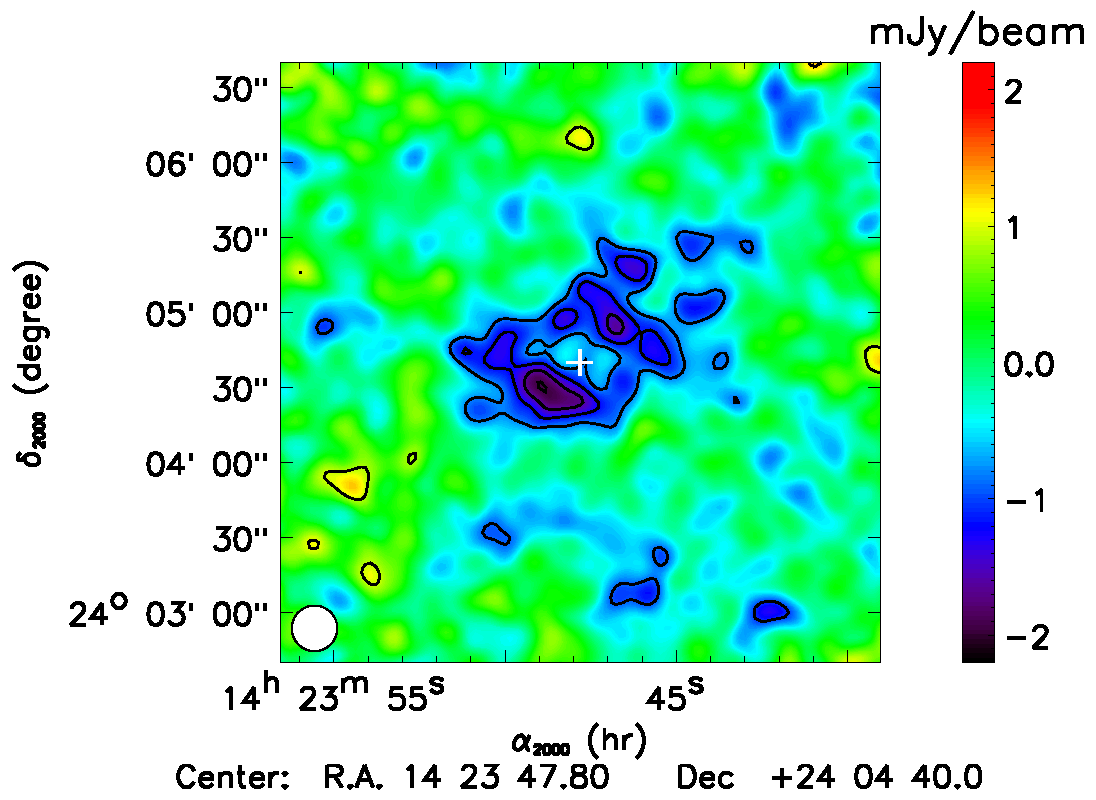
\includegraphics[height=6.6cm]{Figure/MACSJ1424_2mm_map.pdf}
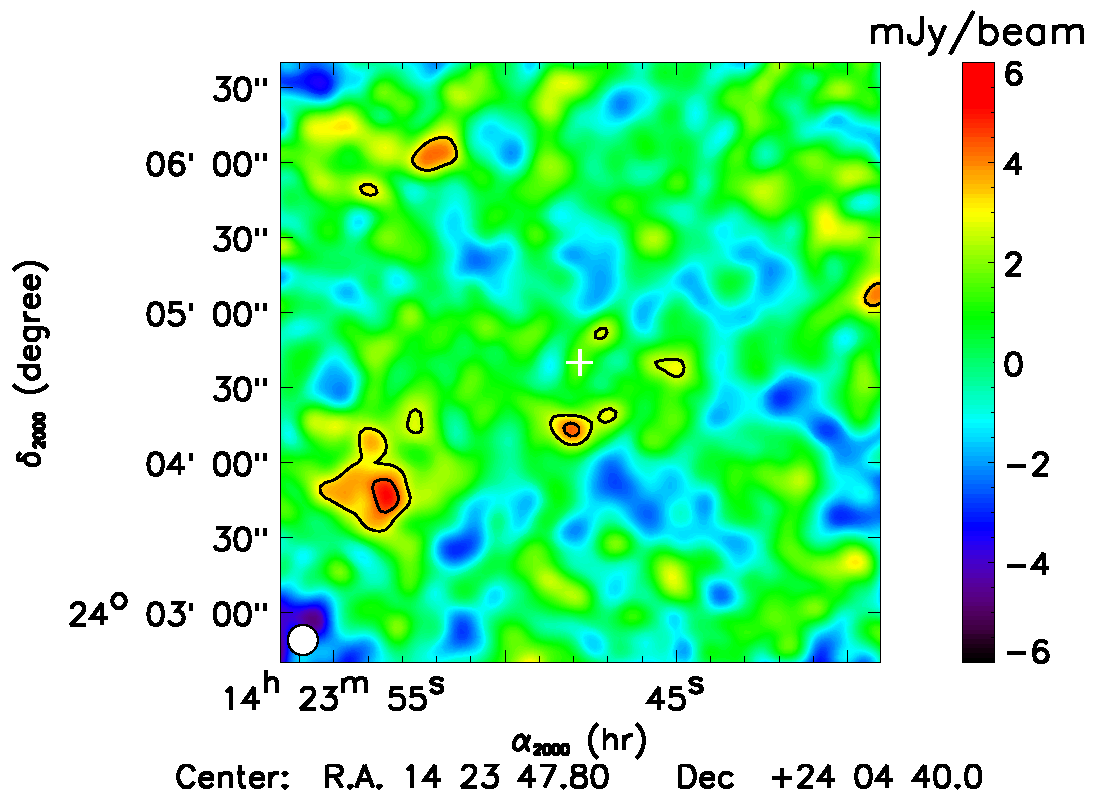
\includegraphics[height=6.6cm]{Figure/MACSJ1424_1mm_map.pdf}
\caption{\DIFaddbeginFL {\footnotesize \DIFaddendFL NIKA maps at 150~GHz (left) and 260~GHz (right) in units of surface brightness. The significance is given by the black contours starting at $\pm 2 \ \sigma$ with 1 $\sigma$ spacing. The maps are smoothed with an extra 10 arcsec Gaussian filter for display \DIFdelbeginFL \DIFdelFL{purpose }\DIFdelendFL \DIFaddbeginFL \DIFaddFL{purposes }\DIFaddendFL and the effective beam FWHM are represented as a white circle in the bottom left corner. The white crosses \DIFdelbeginFL \DIFdelFL{represent }\DIFdelendFL \DIFaddbeginFL \DIFaddFL{indicate }\DIFaddendFL the X-ray center.\DIFaddbeginFL }\DIFaddendFL }
\label{fig:flux_map}
\end{figure*}
The NIKA maps that we obtained are presented in Fig.~\ref{fig:flux_map}. The 150~GHz \DIFdelbegin \DIFdel{one }\DIFdelend \DIFaddbegin \DIFadd{map }\DIFaddend reveals a negative decrement, as expected from the tSZ effect at this frequency, \DIFdelbegin \DIFdel{peaking at }\DIFdelend \DIFaddbegin \DIFadd{with a maximum significance of }\DIFaddend $4.5 \ \sigma$. The morphology of the signal has a ring-like shape, as a consequence of the contamination by the radio point source at the cluster center, which \DIFdelbegin \DIFdel{cancels out }\DIFdelend \DIFaddbegin \DIFadd{fills in }\DIFaddend the tSZ signal. The 260~GHz map does not show any significant tSZ signal. At this frequency, extrapolating from the 150~GHz map, we expect a peak of $\sim 1$ mJy/beam, which is below the level of the noise standard deviation. We observe a $3 \ \sigma$ positive peak around (R.A., Dec.) = (14:23:53, +24:03:45) corresponding to a $2 \ \sigma$ positive peak in the 150~GHz map\DIFdelbegin \DIFdel{. This indicates }\DIFdelend \DIFaddbegin \DIFadd{, due to }\DIFaddend the presence of a sub-millimeter source. Another peak is also seen around (R.A., Dec.) = (+14:23:48, +24:04:15). The radio and sub-millimeter point source contamination will be discussed in \DIFdelbegin \DIFdel{details }\DIFdelend \DIFaddbegin \DIFadd{detail }\DIFaddend in Sect.~\ref{Radio_and_infrared_point_sources}.

%---------- The error bars
The significance of the NIKA maps \DIFdelbegin \DIFdel{is calculated using noise }\DIFdelend \DIFaddbegin \DIFadd{was calculated using }\DIFaddend Monte Carlo realizations. First, a noise map was obtained from the half difference of two equivalent subsets. After having normalized the noise map by the integration time per pixel, the noise spectral distribution was computed using the \DIFdelbegin \DIFdel{POKER }\DIFdelend \DIFaddbegin {\tt \DIFadd{POKER}} \DIFaddend software \citep{ponthieu2011}, which properly accounts for incomplete sky coverage due to the scanning around the cluster. The noise power spectrum was modeled as a function of angular scale $k$, as $P_{\rm noise}(k) = A_{\rm white} + A_{\rm cor}(k_0) \left(\frac{k}{k_0}\right)^{\beta}$. The parameter $A_{\rm white}$ represents the intrinsic detector noise and $A_{\rm cor}$ and $\beta$ give the amplitude and the slope of the \DIFdelbegin \DIFdel{residuals }\DIFdelend \DIFaddbegin \DIFadd{residual }\DIFaddend detector--detector atmospheric correlations in the map. This model was \DIFdelbegin \DIFdel{finally }\DIFdelend used to generate \DIFaddbegin \DIFadd{Monte-Carlo }\DIFaddend noise map realizations, $n_i$, accounting for the integration time per pixel. The noise realizations were smoothed by the same 10~arcsec Gaussian filter used to display the cluster, and the standard deviation across the Monte-Carlo realizations allowed us to compute the root mean square map and therefore the signal to noise contours shown in Fig.~\ref{fig:flux_map}. The full noise covariance matrix was also computed as the mean of the noise covariance over all the realizations, $C = \frac{1}{N_{\rm MC}}\sum_{i=1}^{N_{\rm MC}}n_i n_i^{T}$ and it is used in the analysis \DIFdelbegin \DIFdel{, }\DIFdelend as described in Sect.~\ref{sec:Radial_pressure_reconstruction}.

%###############################################################################################
%##########################                POINT SOURCE CONTAMINATION             ##########################%###############################################################################################
\section{Radio and sub-millimeter point sources}\label{Radio_and_infrared_point_sources}
%========== Radio sources
\subsection{Radio point sources}
VLA (Very Large Array) data  \DIFaddbegin \DIFadd{at 4.8~GHz }\DIFaddend were used by \cite{laroque2003} to detect radio sources towards \mbox{MACS~J1423.8+2404}\DIFdelbegin \DIFdel{at 4.8~GHz}\DIFdelend . Two sources were detected within the NIKA field and we \DIFdelbegin \DIFdel{use }\DIFdelend \DIFaddbegin \DIFadd{used }\DIFaddend the coordinates obtained by \cite{laroque2003} as a reference (see Sect.~\ref{sec:Multi_wavelength_comparison} and Fig.~\ref{fig:MACSJ1424_mutiw}). The first source, hereafter RS1, is located within the central BCG, near the X-ray center. The second\DIFdelbegin \DIFdel{one}\DIFdelend , hereafter RS2, is located at about 1.5 arcmin towards the south-west. The flux of RS1 was measured at various radio wavelengths between 1.4~GHz and 30~GHz while the \DIFdelbegin \DIFdel{one }\DIFdelend \DIFaddbegin \DIFadd{flux }\DIFaddend of RS2 \DIFdelbegin \DIFdel{is only reported }\DIFdelend \DIFaddbegin \DIFadd{has only been measured }\DIFaddend at 1.4 and 4.8~GHz. We list in Table~\ref{tab:Radio_ps} the fluxes measured for both sources \DIFaddbegin \DIFadd{and the corresponding references}\DIFaddend . 
\begin{table*}[h]
\caption{\DIFaddbeginFL {\footnotesize \DIFaddendFL Location and flux of the radio sources observed in the $4 \times 4$ arcmin$^2$ field around \mbox{MACS~J1423.8+2404}.\DIFaddbeginFL }\DIFaddendFL }
\begin{center}
\begin{tabular}{ccccccc}
\hline
\hline
Source & Identifier & Position & 1.4 GHz & 4.8 GHz & 28.5 GHz & 30 GHz \\
 &  & [mJy] & [mJy] & [mJy] & [mJy] \\
\hline
RS1 & NVSS J142347+240439 & 14:23:47.78 +24:04:42.8$^{(a)}$ & $8.0 \pm 1.1 ^{(b)}$ & $4.40 \pm 0.03 ^{(a)}$ & $1.49 \pm 0.12 ^{(c)}$ & $2.0 \pm 0.2 ^{(d)}$ \\
RS2 & NVSS J142345+240340 & 14:23:45.07 +24:03:42.7$^{(a)}$ & $7.2 \pm 0.5 ^{(b)}$ & $2.72 \pm 0.03 ^{(a)}$ &  -- & --  \\  
\hline
\end{tabular}
\end{center}
{\small {\bf Notes.} $^{(a)}$ VLA, \cite{laroque2003}. $^{(b)}$ NVSS, \cite{condon1998}. $^{(c)}$ OVRO/BIMA, \cite{coble2007}. $^{(d)}$ SZA, \cite{bonamente2012}.}
\label{tab:Radio_ps}
\end{table*}

To estimate the expected flux of each source in the NIKA bands, we \DIFdelbegin \DIFdel{model }\DIFdelend \DIFaddbegin \DIFadd{modeled }\DIFaddend their SED by $F_{\nu} = F_{1 \ {\rm GHz}} \left(\frac{\nu}{1 \ {\rm GHz}}\right)^{\alpha_{\rm radio}}$. The fluxes reported in Table~\ref{tab:Radio_ps} \DIFdelbegin \DIFdel{are }\DIFdelend \DIFaddbegin \DIFadd{were }\DIFaddend used to fit the amplitude of the SED, $F_{1 \ {\rm GHz}}$, and its slope, $\alpha_{\rm radio}$. The best-fit parameters are reported in Table~\ref{tab:Radio_ps2} for both sources. We then \DIFdelbegin \DIFdel{simulate mock SED }\DIFdelend \DIFaddbegin \DIFadd{simulated mock SEDs }\DIFaddend by sampling the parameters within their error bars and accounting for the covariance between them. Each mock SED \DIFdelbegin \DIFdel{is }\DIFdelend \DIFaddbegin \DIFadd{was }\DIFaddend then integrated within the NIKA bandpasses to predict the expected flux at 150 and 260~GHz. The histogram of all the realizations \DIFdelbegin \DIFdel{is fitted by }\DIFdelend \DIFaddbegin \DIFadd{was fitted with }\DIFaddend a Gaussian function to give the expected fluxes and uncertainties, which are listed for both sources and both NIKA frequencies in Table~\ref{tab:Radio_ps2}. The values of the spectral index $\alpha_{\rm radio}$ we obtain are typical for radio sources \citep[see for example][]{witzel1979}.
\begin{table*}[h]
\caption{\DIFaddbeginFL \footnotesize \DIFaddendFL Best-fit parameters and extrapolation of the fluxes in the NIKA bands of the radio sources in the $4 \times 4$ arcmin$^2$ field around \mbox{MACS~J1423.8+2404}. The degeneracy between the slope $\alpha_{\rm radio}$ and the amplitude $F_{1 \ {\rm GHz}}$ has been accounted for to extrapolate the flux in the NIKA bands. See text for details.}
\begin{center}
\begin{tabular}{ccccccc}
\hline
\hline
Source & R.A. offset & Dec. offset (arcsec) & $F_{1 \ {\rm GHz}}$ & $\alpha_{\rm radio}$ & 150 GHz & 260 GHz \\
 & [arcsec] & [arcsec] & [mJy] & & [mJy] & [mJy] \\
\hline
RS1 &      0.3 &      2.6 & $   10.39 \pm     0.30$ & $  -0.548 \pm    0.001$ & $    0.68 \pm     0.08$ & $    0.54 \pm     0.07$ \\
RS2 &     41.0 &    -57.3 & $    9.39 \pm     0.69$ & $  -0.790 \pm    0.003$ & $    0.18 \pm     0.04$ & $    0.13 \pm     0.03$ \\
\hline
\end{tabular}
\end{center}
\label{tab:Radio_ps2}
\end{table*}

%DIF < ========== Submm sources
\DIFdelbegin \subsection{\DIFdel{Sub-millimeter point sources}}
%DIFAUXCMD
\addtocounter{subsection}{-1}%DIFAUXCMD
%DIF < ---------- Herschel sources
\DIFdel{We make use of the Herschel satellite SPIRE \mbox{%DIFAUXCMD
\citep{griffin2010} }%DIFAUXCMD
and PACS \mbox{%DIFAUXCMD
\citep{poglitsch2010} }%DIFAUXCMD
data obtained during the Herschel Lensing Survey \mbox{%DIFAUXCMD
\citep[HLS,][]{egami2010,rawle2012}}%DIFAUXCMD
}\footnote{\DIFdel{Obs-IDs 1342188159, 1342188215 and 1342188216.}}%DIFAUXCMD
\addtocounter{footnote}{-1}%DIFAUXCMD
\DIFdel{. They are used to identify sub-millimeter point sources and compute their expected spectral energy distribution (SED) when combined to the NIKA channels, as described below. The Herschel data complement the NIKA ones both in term of wavelengths with 500, 350, 250, 160 and 100 $\mu$m, and angular resolution, FWHM = 35.2, 23.9, 17.6, 9.9, 6.1 arcsec, respectively.
}%DIFDELCMD < 

%DIFDELCMD < %%%
\DIFdel{The PACS maps were produced using the maximum likelihood map maker MADmap \mbox{%DIFAUXCMD
\citep{cantalupo2010}}%DIFAUXCMD
, provided as a PACS Photometer Level 2.5 Product. We use the Herschel Source List Product, generated using the software SUSSEXtractor \mbox{%DIFAUXCMD
\citep{savage2007}}%DIFAUXCMD
, that contains the location and flux of the sources found around \mbox{MACS~J1424.8+2404}. By using all the Herschel frequency bands, we find a total of 17 sub-millimeter sources in the $4 \times 4$ arcmin$^2$ around the cluster. Two of those correspond to the excesses seen in the NIKA 260~GHz map. The 250 $\mu$m channel is the most complete one, with 15 sources, and we use it as a baseline to define the position of the sources and their label. Thus, the corresponding sources in the other channels are identified on the basis of their positions with respect to the 250 $\mu$m ones. Two sources peaking at high frequency are not present in the 250 $\mu$m catalog and we rely on the 100 $\mu$m channel for them. Due to the relatively low resolution at 500 and 350 $\mu$m, a few sources are confused with their neighbors, and in general, all the sources are not available for all the frequency bands in the catalog. Therefore, they are obtained by fitting the amplitude of a Gaussian function on each map, at their reference location. The FWHM is fixed to that of the respective Herschel channels. In addition, we fit also for a local background. In order to account for the confusion in the flux uncertainties, we fit the same Gaussian function at random positions, where the noise is homogeneous, and use the dispersion as the uncertainty. We check that the sources present in the catalog have compatible fluxes with respect to those we recover. The position and fluxes for all the sources are listed in Table~\ref{tab:IR_ps}.
}%DIFDELCMD < 

%DIFDELCMD < %%%
%DIF < ---------- Flux of the sources
\DIFdel{Similarly, the fluxes of the sub-millimeter sources in the NIKA field are obtained by fitting the amplitude of a Gaussian model. We use the NIKA FWHM at the expected sources positions as indicated by the Herschel data. We then correct them for the filtering induced by the data reduction, which is of the order of 15 percent for point sources. Uncertainties are obtained from the standard deviation of the amplitudes recovered using the Gaussian fits performed on the Monte-Carlo noise map realizations. The fluxes obtained and their uncertainties are summarized in Table~\ref{tab:IR_ps} together with the Herschel data. By stacking the flux of all the sources, assuming that they are independent, we obtained an average flux of $1.96 \pm 0.82$ mJy at 260~GHz and $0.46 \pm 0.25$ mJy at 150~GHz, corresponding to a mean detection of 2.4 and 1.9 $ \ \sigma$, respectively. If we exclude the two sources directly detected at the map level, the detection reduces to $1.59 \pm 0.89$ mJy at 260~GHz (1.8 $\sigma$) and $0.45 \pm 0.25$ mJy (1.8 $\sigma$) at 150~GHz.
}\DIFdelend \begin{table*}[h]
\caption{\DIFaddbeginFL \footnotesize \DIFaddendFL Positions and fluxes of the 17 sub-millimeter sources identified in the $4 \times 4$ arcmin$^2$ field around \mbox{MACS~J1423.8+2404}\DIFaddbeginFL \DIFaddFL{, measured by fitting Gaussian models to the maps at each wavelength as described in Sect}\DIFaddendFL .\DIFaddbeginFL \DIFaddFL{~\ref{sec:smmps}. The final two columns correspond to the NIKA bands.}\DIFaddendFL }
\begin{center}
\begin{tabular}{ccccccccc}
\hline
\hline
Source & 250 $\mu$m source position & 100 $\mu$m & 160 $\mu$m & 250 $\mu$m & 350 $\mu$m & 500 $\mu$m & 1.15 mm & 2.05 mm \\
 &  & [mJy] & [mJy] & [mJy] & [mJy] & [mJy] & [mJy] & [mJy] \\
\hline
SMG01 & 14:23:52.31 +24:05:04.9 & $    20.8 \pm      1.1$ & $    35.1 \pm      3.2$ & $    52.3 \pm      7.7$ & $    30.4 \pm      8.1$ & $    11.6 \pm      7.4$ & $     0.6 \pm      3.2$ & $     1.4 \pm      0.9$ \\
SMG02 & 14:23:48.16 +24:04:20.0 & $    12.4 \pm      1.4$ & $    21.0 \pm      3.1$ & $    35.8 \pm      9.8$ & $    24.1 \pm      7.4$ & $    16.3 \pm      7.2$ & $     4.8 \pm      2.9$ & $^{**}$ \\
SMG03 & 14:23:53.50 +24:06:05.1 & $    10.7 \pm      1.2$ & $    17.0 \pm      2.9$ & $    34.7 \pm     11.3$ & $    23.7 \pm      7.9$ & $     8.2 \pm      7.1$ & $     3.4 \pm      3.8$ & $     0.5 \pm      1.1$ \\
SMG04 & 14:23:42.42 +24:04:38.8 & $    11.5 \pm      1.4$ & $    17.7 \pm      3.0$ & $    29.1 \pm     10.8$ & $    21.3 \pm      8.0$ & $     4.4 \pm      7.5$ & $     2.6 \pm      3.2$ & $     0.4 \pm      0.9$ \\
SMG05 & 14:23:47.58 +24:04:48.7 & $     6.1 \pm      1.3$ & $     9.4 \pm      2.8$ & $    25.6 \pm      8.4$ & $    18.3 \pm      7.6$ & $    14.3 \pm      7.5$ & $     3.1 \pm      2.9$ & $^{**}$ \\
SMG06 & 14:23:53.32 +24:03:48.5 & $     2.9 \pm      1.4$ & $     8.5 \pm      3.1$ & $    20.6 \pm      9.6$ & $    14.9 \pm      8.0$ & $     1.8 \pm      7.7$ & $     8.2 \pm      3.4$ & $     1.0 \pm      0.9$ \\
SMG07 & 14:23:45.04 +24:05:48.9 & $     3.4 \pm      1.3$ & $    10.2 \pm      3.0$ & $    20.1 \pm      9.2$ & $    14.0 \pm      8.0$ & $     7.3 \pm      8.0$ & $     1.3 \pm      3.4$ & $     1.0 \pm      0.9$ \\
SMG08 & 14:23:49.16 +24:02:46.1 & $    -1.0 \pm      1.5$ & $     5.4 \pm      3.2$ & $    19.9 \pm      8.8$ & $    24.0 \pm      7.8$ & $    11.2 \pm      7.8$ & $     3.5 \pm      3.8$ & $     0.9 \pm      1.0$ \\
SMG09 & 14:23:43.27 +24:02:50.2 & $     2.4 \pm      1.3$ & $     5.8 \pm      3.3$ & $    12.6 \pm      8.6$ & $    13.8 \pm      7.7$ & $    19.4 \pm      7.8$ & $     2.5 \pm      4.1$ & $    -0.1 \pm      1.1$ \\
SMG10 & 14:23:44.55 +24:03:18.4 & $    -1.5 \pm      1.2$ & $     4.4 \pm      3.3$ & $    11.1 \pm      8.2$ & $    19.0 \pm      7.7$ & $    19.7 \pm      7.8$ & $     4.3 \pm      3.4$ & $    -0.2 \pm      0.9$ \\
SMG11 & 14:23:54.14 +24:05:32.2 & $     7.3 \pm      1.3$ & $    11.6 \pm      2.9$ & $    11.0 \pm      9.1$ & $     3.5 \pm      7.5$ & $     5.9 \pm      7.8$ & $    -1.6 \pm      3.7$ & $     0.3 \pm      1.0$ \\
SMG12 & 14:23:43.41 +24:03:50.6 & $     5.4 \pm      1.3$ & $     9.1 \pm      3.2$ & $     7.3 \pm     10.0$ & $    -1.9 \pm      7.6$ & $    -6.9 \pm      7.4$ & $     2.3 \pm      3.4$ & $     0.4 \pm      0.9$ \\
SMG13 & 14:23:50.13 +24:06:17.4 & $    11.7 \pm      1.3$ & $     8.9 \pm      3.1$ & $     6.4 \pm      7.5$ & $    -2.4 \pm      8.0$ & $   -10.5 \pm      7.7$ & $    -4.2 \pm      3.7$ & $     0.9 \pm      1.0$ \\
SMG14 & 14:23:47.36 +24:05:49.6 & $     3.9 \pm      1.3$ & $     5.5 \pm      2.9$ & $     7.9 \pm      8.6$ & $    10.9 \pm      7.8$ & $     4.7 \pm      7.4$ & $     0.3 \pm      3.2$ & $    -0.2 \pm      0.9$ \\
SMG15 & 14:23:40.95 +24:05:08.7 & $     2.4 \pm      1.3$ & $     3.1 \pm      3.3$ & $     6.6 \pm      9.1$ & $     6.8 \pm      8.2$ & $     8.2 \pm      7.4$ & $    -1.2 \pm      3.5$ & $     0.0 \pm      0.9$ \\
SMG16$^*$  & 14:23:53.69 +24:04:12.6 & $     6.2 \pm      1.4$ & $     7.3 \pm      3.4$ & $    18.0 \pm     10.5$ & $    -4.0 \pm      7.7$ & $    -3.5 \pm      7.5$ & $     3.4 \pm      3.3$ & $     0.6 \pm      0.9$ \\
SMG17$^*$  & 14:23:51.72 +24:05:48.8 & $     4.7 \pm      1.3$ & $     4.3 \pm      3.4$ & $   -14.6 \pm      9.7$ & $    -6.2 \pm      7.7$ & $    -7.4 \pm      7.4$ & $    -2.2 \pm      3.4$ & $    -0.1 \pm      0.9$ \\
\hline
\end{tabular}
\end{center}
{\small {\bf Notes.} $^*$ Sources for which the position is estimated based on the 100 $\mu$m PACS channel. $^{**}$ Fluxes which are not available due to the tSZ contamination.}
\label{tab:IR_ps}
\end{table*}

%DIF > ========== Submm sources
\DIFaddbegin \subsection{\DIFadd{Sub-millimeter point sources}}\label{sec:smmps}
%DIF > ---------- Herschel sources
\DIFadd{We make use of the Herschel  SPIRE \mbox{%DIFAUXCMD
\citep{griffin2010} }%DIFAUXCMD
and PACS \mbox{%DIFAUXCMD
\citep{poglitsch2010} }%DIFAUXCMD
data obtained during the Herschel Lensing Survey \mbox{%DIFAUXCMD
\citep[HLS,][]{egami2010,rawle2012}}%DIFAUXCMD
}\footnote{\DIFadd{Obs-IDs 1342188159, 1342188215 and 1342188216.}} \DIFadd{to identify sub-millimeter point sources and compute their expected spectral energy distribution (SED) as seen by NIKA, as described below. The Herschel data complement those from  NIKA, both in terms of wavelength 500, 350, 250, 160 and 100 $\mu$m, and angular resolution, FWHM = 35.2, 23.9, 17.6, 9.9, 6.1 arcsec, respectively.
}

\DIFadd{The PACS maps were produced using the maximum likelihood map maker MADmap \mbox{%DIFAUXCMD
\citep{cantalupo2010}}%DIFAUXCMD
, provided as a PACS Photometer Level 2.5 Product. We used the Herschel Source List Product, generated using the software SUSSEXtractor \mbox{%DIFAUXCMD
\citep{savage2007}}%DIFAUXCMD
, that contains the location and flux of the sources found around \mbox{MACS~J1424.8+2404}. By using all the Herschel frequency bands, we found a total of 17 sub-millimeter sources in the $4 \times 4$ arcmin$^2$ around the cluster, two of which correspond to the excesses seen in the NIKA 260~GHz map. The 250 $\mu$m channel is the most complete, with 15 sources, and we used it as a baseline to define the source positions and labels; the corresponding sources in the other channels were identified on the basis of their positions with respect to those in the 250 $\mu$m channel. Two sources peaking at high frequency were not present in the 250 $\mu$m catalog and we relied on the 100 $\mu$m channel for their properties. Due to the relatively low resolution at 500 and 350 $\mu$m, a few sources are confused with their neighbors, and in general, not all the sources are identifiable in all the frequency bands in the catalog. To obtain the fluxes of all sources in all bands, we fit the amplitude of a Gaussian function to each map, with position fixed at the source reference location and FWHM fixed to that of the respective Herschel channels. A local background was also fit. In order to account for the confusion in the flux uncertainties, we fit the same Gaussian function at random positions, where the noise is homogeneous, and use the dispersion as the uncertainty. We checked that the sources present in the catalog have compatible fluxes with respect to those we recovered. The positions and fluxes for all the sources are listed in Table~\ref{tab:IR_ps}.
}

%DIF > ---------- Flux of the sources
\DIFadd{Similarly, the fluxes of the sub-millimeter sources in the NIKA field were obtained by fitting the amplitude of a Gaussian model, using the NIKA FWHM at the source positions expected from Herschel data. These were then corrected them for the filtering induced by the data reduction ($\sim15$ percent for point sources). Uncertainties were obtained from the standard deviation of the amplitudes recovered using Gaussian fits performed on the Monte-Carlo noise map realizations. The fluxes obtained and their uncertainties are summarized together with the Herschel data in columns Table~\ref{tab:IR_ps}. By stacking the flux of all the sources, assuming that they are independent, we obtained an average flux of $1.96 \pm 0.82$ mJy at 260~GHz (1.15~mm) and $0.46 \pm 0.25$ mJy at 150~GHz (2.05~mm), corresponding to a mean detection of 2.4 and 1.9 $ \ \sigma$, respectively. If we exclude the two sources directly detected at the map level, the detection reduces to $1.59 \pm 0.89$ mJy at 260~GHz (1.8 $\sigma$) and $0.45 \pm 0.25$ mJy (1.8 $\sigma$) at 150~GHz.
}

\DIFaddend \begin{table*}[h]
\caption{\DIFaddbeginFL \footnotesize \DIFaddendFL Offset with respect to the X-ray center, and flux extrapolated to the NIKA channels for the 17 sub-millimeter sources identified in the $4 \times 4$ arcmin$^2$ field around \mbox{MACS~J1423.8+2404}\DIFaddbeginFL \DIFaddFL{, obtained from the SED model described in Sect}\DIFaddendFL .\DIFaddbeginFL \DIFaddFL{~\ref{sec:smmps}. }\DIFaddendFL Despite \DIFdelbeginFL \DIFdelFL{there }\DIFdelendFL \DIFaddbeginFL \DIFaddFL{the }\DIFaddendFL large uncertainties, these values allow to \DIFaddbeginFL \DIFaddFL{us }\DIFaddendFL estimate the impact of the \DIFdelbeginFL \DIFdelFL{contaminant }\DIFdelendFL \DIFaddbeginFL \DIFaddFL{contaminating }\DIFaddendFL sources on the reconstructed cluster \DIFdelbeginFL \DIFdelFL{physics}\DIFdelendFL \DIFaddbeginFL \DIFaddFL{properties}\DIFaddendFL .}
\begin{center}
\begin{tabular}{ccccccc}
\hline
\hline
Source &  R.A. offset & Dec. offset & 1.15 mm \DIFaddbeginFL \DIFaddFL{/ 260~GHz }\DIFaddendFL & 2.05 mm \DIFaddbeginFL \DIFaddFL{/ 150~GHz}\DIFaddendFL \\
 &  [arcsec] & [arcsec] & [mJy] & [mJy] \\
\hline
SMG01 &    -61.8 &     24.9 & $    1.52 \pm     0.64$ & $    0.30 \pm     0.19$ \\
SMG02 &     -5.0 &    -20.0 & $    2.39 \pm     1.10$ & $    0.62 \pm     0.42$ \\
SMG03 &    -78.1 &     85.1 & $    1.51 \pm     0.79$ & $    0.35 \pm     0.26$ \\
SMG04 &     73.7 &     -1.2 & $    1.05 \pm     0.67$ & $    0.25 \pm     0.21$ \\
SMG05 &      3.0 &      8.7 & $    2.01 \pm     0.97$ & $    0.50 \pm     0.34$ \\
SMG06 &    -75.5 &    -51.5 & $    1.13 \pm     1.12$ & $    0.31 \pm     0.39$ \\
SMG07 &     37.8 &     68.9 & $    0.60 \pm     0.57$ & $    0.15 \pm     0.17$ \\
SMG08 &    -18.6 &   -113.9 & $    2.53 \pm     1.17$ & $    0.60 \pm     0.40$ \\
SMG09 &     62.1 &   -109.8 & $    2.15 \pm     1.51$ & $    0.55 \pm     0.47$ \\
SMG10 &     44.5 &    -81.6 & $    3.79 \pm     1.56$ & $    0.97 \pm     0.55$ \\
SMG11 &    -86.8 &     52.2 & $    0.09 \pm     0.12$ & $    0.02 \pm     0.03$ \\
SMG12 &     60.1 &    -49.4 & $    0.05 \pm     0.07$ & $    0.01 \pm     0.02$ \\
SMG13 &    -31.9 &     97.4 & $    0.05 \pm     0.06$ & $    0.01 \pm     0.01$ \\
SMG14 &      6.1 &     69.6 & $    0.14 \pm     0.23$ & $    0.03 \pm     0.06$ \\
SMG15 &     93.8 &     28.7 & $    0.13 \pm     0.28$ & $    0.03 \pm     0.07$ \\
SMG16$^*$ &    -80.6 &    -27.4 & $    0.08 \pm     0.11$ & $    0.02 \pm     0.03$ \\
SMG17$^*$ &    -53.6 &     68.8 & $    0.03 \pm     0.04$ & $    0.01 \pm     0.01$ \\
\hline
\end{tabular}
\end{center}
{\small {\bf Notes.} $^*$ Sources for which the position is estimated based on the 100 $\mu$m PACS channel.}
\label{tab:IR_ps2}
\end{table*}

%---------- Modeling and fit of the SED
Only SMG02 and SMG06 are directly detected in the NIKA maps. \DIFdelbegin \DIFdel{In order to }\DIFdelend \DIFaddbegin \DIFadd{To }\DIFaddend better constrain the fluxes \DIFdelbegin \DIFdel{within }\DIFdelend \DIFaddbegin \DIFadd{in }\DIFaddend the NIKA bands, we \DIFdelbegin \DIFdel{model the SED by }\DIFdelend \DIFaddbegin \DIFadd{modeled the SED with }\DIFaddend a modified black-body spectrum, $F_{\nu} = A_0 \left(\frac{\nu}{\nu_0}\right)^{\beta_{\rm dust}} B_{\nu}(T_{\rm dust})$\DIFdelbegin \DIFdel{. The parameter }\DIFdelend \DIFaddbegin \DIFadd{, where }\DIFaddend $A_0$ is a normalization, $\nu_0$ a reference frequency, $\beta_{\rm dust}$ the dust spectral index and $T_{\rm dust}$ the dust temperature. We \DIFdelbegin \DIFdel{notice }\DIFdelend \DIFaddbegin \DIFadd{noticed }\DIFaddend a flux excess at 100 $\mu$m for most of the sources with respect to the best-fit SED derived from all the other channels, which we attribute to \DIFdelbegin \DIFdel{a too simplistic }\DIFdelend \DIFaddbegin \DIFadd{the modified black-body spectrum being too simplistic a }\DIFaddend description of the data \DIFdelbegin \DIFdel{by modified black-body spectrum }\DIFdelend at high frequency. We therefore \DIFdelbegin \DIFdel{exclude }\DIFdelend \DIFaddbegin \DIFadd{excluded }\DIFaddend this frequency for constraining the SED in the following. Since we aim \DIFdelbegin \DIFdel{at subtracting }\DIFdelend \DIFaddbegin \DIFadd{to subtract }\DIFaddend the sources at 150~GHz, we also \DIFdelbegin \DIFdel{exclude }\DIFdelend \DIFaddbegin \DIFadd{excluded }\DIFaddend the NIKA measurement at this frequency and only \DIFdelbegin \DIFdel{check }\DIFdelend \DIFaddbegin \DIFadd{checked }\DIFaddend that predicted and measured fluxes are consistent. For \DIFaddbegin \DIFadd{the }\DIFaddend SMG02 and SMG05 sources, the 150~GHz data \DIFdelbegin \DIFdel{have not been }\DIFdelend \DIFaddbegin \DIFadd{were not }\DIFaddend extracted because of strong contamination by the local tSZ signal.

We \DIFdelbegin \DIFdel{perform a Markov Chains }\DIFdelend \DIFaddbegin \DIFadd{performed a Markov Chain }\DIFaddend Monte Carlo (MCMC) analysis to fit simultaneously for $\beta_{\rm dust}$ and $T_{\rm dust}$. This \DIFaddbegin \DIFadd{approach }\DIFaddend allows us to sample the corresponding parameter space and \DIFaddbegin \DIFadd{to }\DIFaddend automatically marginalize over $A_0$, which is highly \DIFdelbegin \DIFdel{degenerated }\DIFdelend \DIFaddbegin \DIFadd{degenerate }\DIFaddend with the two other parameters. The Metropolis-Hasting algorithm \DIFdelbegin \DIFdel{is }\DIFdelend \DIFaddbegin \DIFadd{was }\DIFaddend used to sample the parameter space. Each model tested against the data \DIFdelbegin \DIFdel{is }\DIFdelend \DIFaddbegin \DIFadd{was }\DIFaddend defined by a value of $\beta_{\rm dust}$ and $T_{\rm dust}$ and the normalization \DIFdelbegin \DIFdel{is linearly adjusted }\DIFdelend \DIFaddbegin \DIFadd{was linearly fit }\DIFaddend to the data. For NIKA, color corrections are expected to be negligible with respect to the calibration and statistical uncertainties ($\sim 1-2$\%). In the case of Herschel, we apply the color corrections given in \cite{poglitsch2010} for PACS and those available in the online documentation for SPIRE\footnote{\url{http://herschel.esac.esa.int/Docs/SPIRE/html/spire_om.html\#x1-830005.2.6}}. These coefficients \DIFdelbegin \DIFdel{are }\DIFdelend \DIFaddbegin \DIFadd{were }\DIFaddend interpolated for each model using the values of $\beta_{\rm dust}$ and $T_{\rm dust}$, and provide a small correction to the Herschel fluxes ($\sim 5-10$\%). We finally \DIFdelbegin \DIFdel{obtain }\DIFdelend \DIFaddbegin \DIFadd{obtained }\DIFaddend a set of models distributed with respect to the posterior likelihood. Each of the model SED spectra \DIFdelbegin \DIFdel{is }\DIFdelend \DIFaddbegin \DIFadd{was }\DIFaddend integrated within the NIKA bandpasses\DIFdelbegin \DIFdel{and }\DIFdelend \DIFaddbegin \DIFadd{, with }\DIFaddend the distribution of fluxes \DIFdelbegin \DIFdel{gives }\DIFdelend \DIFaddbegin \DIFadd{giving }\DIFaddend the expected value and \DIFdelbegin \DIFdel{its }\DIFdelend uncertainty. The results are summarized in Table~\ref{tab:IR_ps2}.

%========== Surface brightness profile
\subsection{Surface brightness profile}\label{sec:surface_brightness_profiles_comparison}
%---------- Method
\DIFdelbegin \DIFdel{Using the maps of Fig.~\ref{fig:flux_map} we compute }\DIFdelend \DIFaddbegin \DIFadd{Figure~\ref{fig:flux_profiles}  shows }\DIFaddend the flux density profiles \DIFdelbegin \DIFdel{shown in Fig.~\ref{fig:flux_profiles} }\DIFdelend \DIFaddbegin \DIFadd{at 150 and 260~GHz, obtained }\DIFaddend by averaging the signal \DIFdelbegin \DIFdel{within }\DIFdelend \DIFaddbegin \DIFadd{from the NIKA maps in Fig.~\ref{fig:flux_map} in }\DIFaddend radial bins around the X-ray center.  
\DIFdelbegin \DIFdel{The error bars are }\DIFdelend %DIF > Using the maps of Fig.~\ref{fig:flux_map} we computed the flux density profiles shown in Fig.~\ref{fig:flux_profiles} by averaging the signal within radial bins around the X-ray center. 
\DIFaddbegin \DIFadd{Uncertainties were }\DIFaddend computed by using the noise realizations described in Sect.~\ref{sec:Raw_NIKA_observations}\DIFdelbegin \DIFdel{. A }\DIFdelend \DIFaddbegin \DIFadd{: the }\DIFaddend flux density profile \DIFdelbegin \DIFdel{is }\DIFdelend \DIFaddbegin \DIFadd{was }\DIFaddend computed for each noise realization and the standard deviation of all the realizations per radial bin \DIFdelbegin \DIFdel{provide the error bars associated to the profiles}\DIFdelend \DIFaddbegin \DIFadd{provided the associated error bars}\DIFaddend . This allows us to account for pixel--pixel noise correlation. We also \DIFdelbegin \DIFdel{compute }\DIFdelend \DIFaddbegin \DIFadd{computed }\DIFaddend the profile expected from the point sources for each NIKA band \DIFdelbegin \DIFdel{. This is done }\DIFdelend by simulating the corresponding maps using the point source fluxes and positions given in Tables~\ref{tab:Radio_ps2} and~\ref{tab:IR_ps2}. The profile \DIFdelbegin \DIFdel{is }\DIFdelend \DIFaddbegin \DIFadd{was }\DIFaddend then calculated as for the NIKA maps and the error \DIFdelbegin \DIFdel{is }\DIFdelend given by the dispersion of Monte Carlo realizations of the point source maps by randomly varying \DIFdelbegin \DIFdel{the fluxes within their }\DIFdelend \DIFaddbegin \DIFadd{their fluxes within the }\DIFaddend Gaussian errors.

%---------- 150GHz
\DIFdelbegin \DIFdel{Fig.~\ref{fig:flux_profiles} shows that the }\DIFdelend \DIFaddbegin \DIFadd{The }\DIFaddend 150~GHz profile decreases smoothly towards the center, due to the tSZ signal, except in the inner 15 arcsec, were it rises. This is consistent with the positive signal expected from the \DIFdelbegin \DIFdel{point-like sources, dominated by the radio and the }\DIFdelend \DIFaddbegin \DIFadd{presence of radio and }\DIFaddend sub-millimeter \DIFdelbegin \DIFdel{ones }\DIFdelend \DIFaddbegin \DIFadd{emission from point-like sources }\DIFaddend in the cluster core. \DIFdelbegin \DIFdel{The }\DIFdelend \DIFaddbegin \DIFadd{Outside the core, the }\DIFaddend cluster is detected, at the profile level, up to 60 arcsec radius. 

%---------- 260GHz
\DIFdelbegin \DIFdel{We notice that the }\DIFdelend \DIFaddbegin \DIFadd{The }\DIFaddend sub-millimeter sources shown in Fig.~\ref{fig:MACSJ1424_mutiw} are located in two distinct regions. Two of them are within 30 arcsec from the X-ray peak, where we expect the tSZ contribution to be the strongest, while the others are concentrated in a ring of 70 arcsec inner radius and 130 arcsec outer radius. No source is seen around 50 arcsec from the cluster center. \DIFdelbegin \DIFdel{Despite the large error bars at }\DIFdelend \DIFaddbegin \DIFadd{This source distribution is reproduced, despite the large uncertainties, in the }\DIFaddend 260~GHz \DIFdelbegin \DIFdel{, we see }\DIFdelend \DIFaddbegin \DIFadd{profile. There is }\DIFaddend an excess near the center which we attribute to the sum of tSZ and sub-millimeter sources (\DIFdelbegin \DIFdel{from which one of  them }\DIFdelend \DIFaddbegin \DIFadd{one of  which }\DIFaddend is detected with NIKA at the map level). A dip \DIFdelbegin \DIFdel{is }\DIFdelend \DIFaddbegin \DIFadd{can be  }\DIFaddend seen around 1 arcmin, \DIFdelbegin \DIFdel{as expected from the sources distribution, }\DIFdelend and another excess is seen around 100 arcsec from the center, \DIFdelbegin \DIFdel{attributed again to the Herschel sources. The }\DIFdelend \DIFaddbegin \DIFadd{both due to the distribition of Herschel point sources. Overall, the }\DIFaddend NIKA 260~GHz profile is consistent with that expected from \DIFdelbegin \DIFdel{point sources.
}\DIFdelend \DIFaddbegin \DIFadd{the observed point source distribition.
}

\DIFaddend \begin{figure*}[h]
\centering
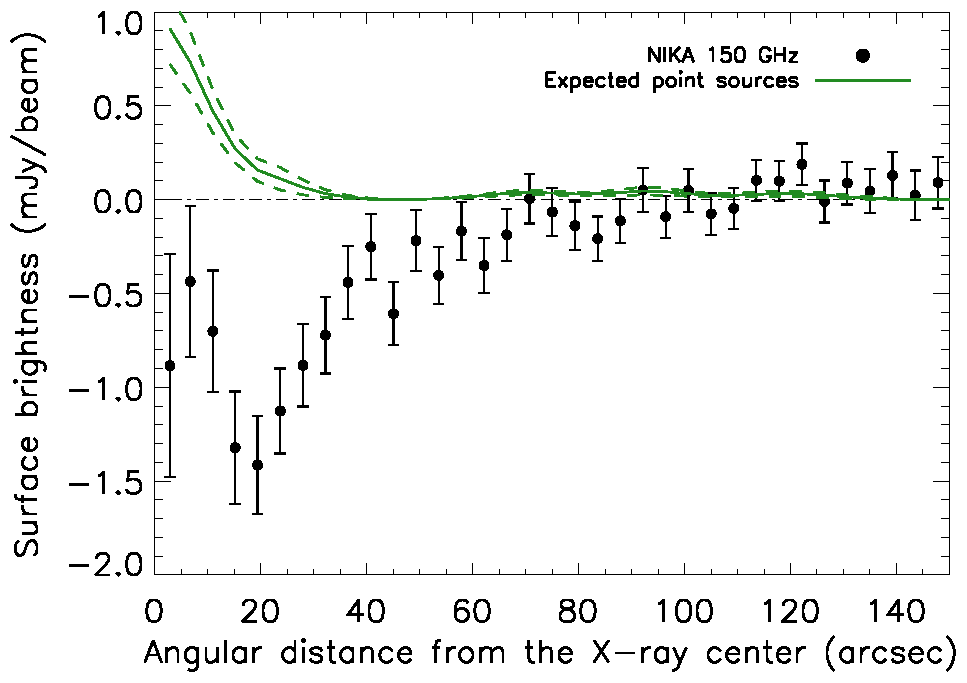
\includegraphics[height=6.4cm]{Figure/MACSJ1424_profile2mm_plus_ps.pdf}
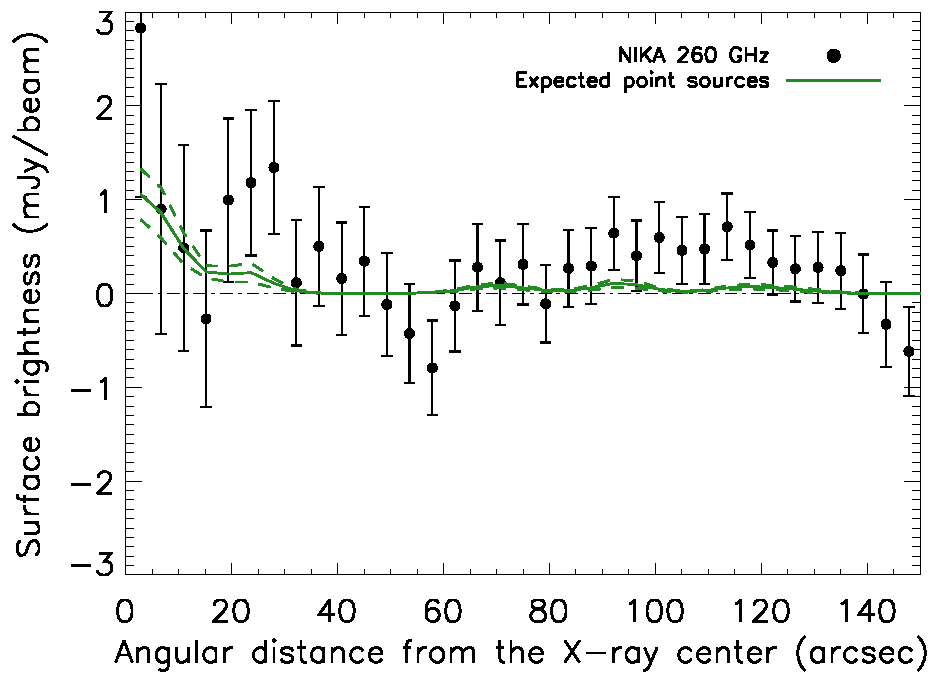
\includegraphics[height=6.4cm]{Figure/MACSJ1424_profile1mm_plus_ps.pdf}
\caption{\DIFaddbeginFL \footnotesize \DIFaddendFL Profiles at 150~GHz (left) and 260~GHz (right), in units of surface brightness, of the raw map (black dots) and the contribution expected from radio and sub-millimeter point sources (green solid line). The green dashed envelope gives the 68\% confidence interval on the point \DIFdelbeginFL \DIFdelFL{sources }\DIFdelendFL \DIFaddbeginFL \DIFaddFL{source }\DIFaddendFL profile.}
\label{fig:flux_profiles}
\end{figure*}

%###############################################################################################
%##########################                              XRAY ANALYSIS                             ##########################%###############################################################################################
\section{XMM-Newton and Chandra X-ray data reduction}\label{sec:XMM_Newton_and_Chandra_X_ray_data_reduction}
X-ray observations of galaxy clusters are sensitive to both the electronic density and the temperature of the ICM. The X-ray surface brightness is expressed as 
\begin{equation}
	S_X = \frac{1}{4 \pi \left(1+z\right)^4} \int n_e^2 \Lambda(T_e, Z) \ dl,
	\label{eq:sx}
\end{equation}
where $\Lambda(T_e,Z)$ is the cooling function, which depends on the temperature and the ICM metallicity $Z$, and is roughly proportional to $T_e^{1/2}$. While X-ray imaging is mainly sensitive to the electronic density, the gas temperature can be estimated from X-ray spectroscopy. See for example \cite{bohringer2010} for a review.

%==========  Data prep.
\subsection{Data preparation}
\DIFdelbegin \DIFdel{The cluster }\DIFdelend \mbox{MACS~J1423.8+2404} was observed by the Chandra Advanced CCD Imaging Spectrometer (ACIS) for \SI{115}{\kilo\second} (obs-ID $4195$) and by the XMM-Newton European Photon Imaging Camera (EPIC) for $\SI{109}{\kilo\second}$ in total (obs-IDs $720700301$ and $720700401$). XMM-Newton datasets were \DIFdelbegin \DIFdel{re-processed, }\DIFdelend \DIFaddbegin \DIFadd{processed by }\DIFaddend applying the latest calibration files, using the Science Analysis System (SAS) version $14.0.0$ and \DIFdelbegin \DIFdel{calibrations files as }\DIFdelend \DIFaddbegin \DIFadd{the calibration files }\DIFaddend available in May $2015$. Chandra datasets were \DIFdelbegin \DIFdel{re-processed }\DIFdelend \DIFaddbegin \DIFadd{processed }\DIFaddend using the Chandra Interactive Analysis of Observation (CIAO) software suite version $4.7$ and calibration database version $4.6.5$. To reduce contamination from the stationary flux of high energetic particles we applied the Very Faint mode\footnote{\label{fn1}\url{http://cxc.cfa.harvard.edu/cal/Acis/Cal\_prods/vfbkgrnd/}} filtering to \DIFdelbegin \DIFdel{Chandra datasets and for }\DIFdelend \DIFaddbegin \DIFadd{the Chandra datasets. For }\DIFaddend XMM-Newton\DIFaddbegin \DIFadd{, }\DIFaddend we rejected events for which the keyword \DIFdelbegin \DIFdel{PATTERN (see, e.g., \mbox{%DIFAUXCMD
\citealt{pratt2007}}%DIFAUXCMD
) }\DIFdelend \DIFaddbegin {\sc \DIFadd{pattern}}  \DIFaddend is $> 4$ (for MOS$1,2$) and $>13$ (for PN). %DIF >  (see, e.g., \citealt{pratt2007}).

\DIFaddbegin \DIFadd{The }\DIFaddend Chandra and XMM-Newton datasets were analyzed using the \DIFdelbegin \DIFdel{very same techniqueso, }\DIFdelend \DIFaddbegin \DIFadd{same technique, so }\DIFaddend unless otherwise stated, the procedures described in the following were applied to both datasets. To remove \DIFaddbegin \DIFadd{solar soft proton }\DIFaddend flare contamination we followed the procedures described in \cite{pratt2007} and in the Chandra \DIFdelbegin \DIFdel{COOKBOOK}\DIFdelend \DIFaddbegin {\sc \DIFadd{cookbook}}\DIFaddend \footnote{\label{fn2}\url{http://cxc.harvard.edu/contrib/maxim/acisbg/COOKBOOK}} for \DIFaddbegin \DIFadd{the }\DIFaddend XMM-Newton and Chandra datasets, respectively, rejecting time intervals where the count rate \DIFdelbegin \DIFdel{exceeds }\DIFdelend \DIFaddbegin \DIFadd{exceeded }\DIFaddend $3 \ \sigma$ with respect to the mean value. \DIFdelbegin \DIFdel{After the cleaning procedure we }\DIFdelend \DIFaddbegin \DIFadd{We }\DIFaddend found no flare contamination in the Chandra dataset, \DIFdelbegin \DIFdel{and a }\DIFdelend \DIFaddbegin \DIFadd{thus the full 115~ks observation was used; for the XMM-Newton dataset, the }\DIFaddend useful exposure time \DIFdelbegin \DIFdel{of }\DIFdelend \DIFaddbegin \DIFadd{was }\DIFaddend $\SI{122}{\kilo\second}$ for MOS$1$+MOS$2$ and $\SI{41}{\kilo\second}$ for PN. To identify point sources we ran a wavelet detection algorithm with a threshold of $5 \ \sigma$ on exposure corrected images in the \DIFdelbegin \DIFdel{$[0.3-2] \ \si{\kilo\electronvolt}$ and in }\DIFdelend $[0.7-7] \ \si{\kilo\electronvolt}$ \DIFdelbegin \DIFdel{bands for the }\DIFdelend \DIFaddbegin \DIFadd{and $[0.3-2] \ \si{\kilo\electronvolt}$ bands }\DIFaddend Chandra and XMM-Newton\DIFdelbegin \DIFdel{datasets}\DIFdelend , respectively. The \DIFdelbegin \DIFdel{list of sources identified in both datasets }\DIFdelend \DIFaddbegin \DIFadd{resulting source lists }\DIFaddend were merged, inspected by eye and used as a mask to remove point source contributions from the analysis.

%==========  Vignetting correction
\subsection{Vignetting correction}
To correct for vignetting, we followed the procedure described in \cite{arnaud2001}, computing \DIFaddbegin \DIFadd{a weight }\DIFaddend for each photon\DIFdelbegin \DIFdel{a weight }\DIFdelend \DIFaddbegin \DIFadd{, }\DIFaddend defined as the ratio of the effective area at the aimpoint \DIFdelbegin \DIFdel{and }\DIFdelend \DIFaddbegin \DIFadd{to that }\DIFaddend at the photon position. Using these quantities, we can perform imaging and spectroscopic analysis as if the detector had a flat response equal to that at the aimpoint. \DIFdelbegin \DIFdel{The }\DIFdelend \DIFaddbegin \DIFadd{For XMM-Newton, the }\DIFaddend weights were computed using the \verb?evigweight? routine\DIFdelbegin \DIFdel{for XMM-Newton, while for }\DIFdelend \DIFaddbegin \DIFadd{; for }\DIFaddend Chandra we used the procedure described in \textcolor{blue}{Bartalucci et al. (in \DIFdelbegin \DIFdel{preparation}\DIFdelend \DIFaddbegin \DIFadd{prep.}\DIFaddend )}. For each photon we also computed the effective exposure time, producing exposure maps that take into account bad pixels and columns. \DIFdelbegin \DIFdel{All the }\DIFdelend \DIFaddbegin \DIFadd{The }\DIFaddend response files for weights and spectroscopic analysis were computed using the appropriate \DIFdelbegin \DIFdel{CIAO, }\DIFdelend \DIFaddbegin \DIFadd{tools in CIAO (}\DIFaddend \verb?mkarf? and \verb?mkacisrmf?\DIFdelbegin \DIFdel{, and SAS , }\DIFdelend \DIFaddbegin \DIFadd{) and SAS (}\DIFaddend \verb?arfgen? and \verb?rmfgen?\DIFdelbegin \DIFdel{, tools}\DIFdelend \DIFaddbegin \DIFadd{)}\DIFaddend .

%==========  Background subtraction
\subsection{Background subtraction}
The X-ray background is due to \DIFdelbegin \DIFdel{a }\DIFdelend diffuse sky emission and an instrumental component caused by the interaction of \DIFdelbegin \DIFdel{stationary }\DIFdelend high energetic particles with telescope instruments. To estimate the latter\DIFdelbegin \DIFdel{component}\DIFdelend , we used datasets tailored to isolate this component, namely \DIFdelbegin \DIFdel{CLOSED (see \mbox{%DIFAUXCMD
\citealt{pratt2009}}%DIFAUXCMD
) and STOWED}\DIFdelend \DIFaddbegin {\sc \DIFadd{closed}} \DIFadd{and }{\sc \DIFadd{stowed}} \DIFaddend \footref{fn2} for XMM-Newton and Chandra, respectively. To match the observation, these datasets \DIFdelbegin \DIFdel{are }\DIFdelend \DIFaddbegin \DIFadd{were  }\DIFaddend skycasted and normalized in the $[10-12], \ [12-14] \ \si{\kilo\electronvolt}$ and in the $[9.5-10.6] \ \si{\kilo\electronvolt}$ band for MOS$1,2$-PN and ACIS, respectively. For Chandra we \DIFdelbegin \DIFdel{chose }\DIFdelend \DIFaddbegin \DIFadd{used }\DIFaddend background datasets from period D, since the observation was performed in \DIFdelbegin \DIFdel{2003, as discussed in the COOKBOOK}%DIFDELCMD < \footref{fn2}%%%
\DIFdel{. }\DIFdelend \DIFaddbegin \DIFadd{2003. }\DIFaddend We computed the weights for the instrumental background datasets \DIFaddbegin \DIFadd{by }\DIFaddend applying the same point source masking and filtering procedures as for the observation datasets. We then subtracted from the surface brightness and temperature profiles the instrumental background evaluated using these datasets.

The residual background component is composed of \DIFdelbegin \DIFdel{a }\DIFdelend thermal Galactic emission \citep{snowden1995} and the blending of unresolved distant point sources, known as the cosmic X-ray background \citep{giacconi2001}. For the surface brightness profile analysis we determine a region free from cluster emission and subtract the residual mean background count rate. For the spectroscopic analysis we extracted the spectrum from the \DIFdelbegin \DIFdel{source free }\DIFdelend \DIFaddbegin \DIFadd{source-free }\DIFaddend region and fitted it \DIFdelbegin \DIFdel{, through maximum likelihood estimation, with a multi component model , composed by two absorbed MEKAL }\DIFdelend \DIFaddbegin \DIFadd{with a multi-component model composed of two absorbed }{\sc \DIFadd{MEKAL}} \DIFadd{thermal components }\DIFaddend and an absorbed power law (for details on the model used, see \citealt{pratt2009}). \DIFdelbegin \DIFdel{The X-ray spectra in this work were extracted in the $[0.7-10] \ \si{\kilo\electronvolt}$ and in the $[0.3-10] \ \si{\kilo\electronvolt}$ band for Chandra and XMM-Newton datasets, respectively. }\DIFdelend When performing further spectroscopic analysis we added the background model as a fixed component\DIFdelbegin \DIFdel{whose amplitude is }\DIFdelend \DIFaddbegin \DIFadd{, with an amplitude }\DIFaddend scaled by the ratio of the \DIFaddbegin \DIFadd{area of the }\DIFaddend region of interest \DIFdelbegin \DIFdel{and }\DIFdelend \DIFaddbegin \DIFadd{to that of the source-free }\DIFaddend background area. \DIFaddbegin \DIFadd{The X-ray spectra were extracted and analysed in the $[0.3-10] \ \si{\kilo\electronvolt}$ and $[0.7-10] \ \si{\kilo\electronvolt}$ bands for XMM-Newton and Chandra, respectively. 
}\DIFaddend 

%###############################################################################################
%##########################              MULTI WAVELENGTH COMPARISON            ##########################%###############################################################################################
\section{Multi-wavelength comparison}\label{sec:Multi_wavelength_comparison}
\DIFdelbegin \DIFdel{The data used in the present work are gathered in }\DIFdelend Fig.~\ref{fig:MACSJ1424_mutiw2} \DIFdelbegin \DIFdel{. Even if the map is not directly used in itself, we also give the FIRST survey }\DIFdelend \DIFaddbegin \DIFadd{presents a multi-wavelength overview of \mbox{MACS~J1423.8+2404}, including the }{\sc \DIFadd{first}} \DIFadd{survey \mbox{%DIFAUXCMD
\citep[Faint Images of the Radio Sky at Twenty-Centimeters,][]{becker1995} }%DIFAUXCMD
}\DIFaddend observations at 1.4~GHz \DIFdelbegin \DIFdel{\mbox{%DIFAUXCMD
\citep[Faint Images of the Radio Sky at Twenty-Centimeters,][]{becker1995}}%DIFAUXCMD
, which provides }\DIFdelend \DIFaddbegin \DIFadd{that provided }\DIFaddend the radio point \DIFdelbegin \DIFdel{sources }\DIFdelend \DIFaddbegin \DIFadd{source }\DIFaddend locations. The two radio sources \DIFdelbegin \DIFdel{are }\DIFdelend \DIFaddbegin \DIFadd{discussed in Sect.~\ref{sec:smmps} are clearly }\DIFaddend visible on the map. \DIFdelbegin \DIFdel{Focussing on Herschel and NIKA data, the }\DIFdelend \DIFaddbegin \DIFadd{The }\DIFaddend complementarity of the \DIFdelbegin \DIFdel{two instruments appears clearly. Indeed}\DIFdelend \DIFaddbegin \DIFadd{Herschel and NIKA instruments is clear}\DIFaddend , the NIKA bands \DIFdelbegin \DIFdel{complement }\DIFdelend \DIFaddbegin \DIFadd{complementing }\DIFaddend the Herschel spectral coverage at lower frequencies. In addition, the angular resolution of the NIKA bands is comparable to \DIFdelbegin \DIFdel{the }\DIFdelend \DIFaddbegin \DIFadd{that of SPIRE at }\DIFaddend 250 $\mu$m \DIFdelbegin \DIFdel{SPIRE and }\DIFdelend \DIFaddbegin \DIFadd{and PACS at }\DIFaddend 160 $\mu$m\DIFdelbegin \DIFdel{PACS ones, allowing }\DIFdelend \DIFaddbegin \DIFadd{, allowing us }\DIFaddend to break the confusion in the low frequency \DIFdelbegin \DIFdel{bands of SPIRE in crowded environment, such as galaxy clusters}\DIFdelend \DIFaddbegin \DIFadd{SPIRE bands in the crowded cluster environment}\DIFaddend . The HST (Hubble Space Telescope) data from the CLASH program \citep[][Cluster Lensing And Supernova survey with Hubble]{postman2012} \DIFdelbegin \DIFdel{are represented for visual comparison but are not used directly in the present work. They allow to }\DIFdelend show the galaxy distribution. The \DIFdelbegin \DIFdel{X-ray Chandra image is represented to trace }\DIFdelend \DIFaddbegin \DIFadd{(smoothed) Chandra X-ray image traces }\DIFaddend the gas electronic density and will be used further in Sect.~\ref{sec:Radial_pressure_reconstruction}.
\DIFaddbegin 

\DIFaddend \begin{figure*}[h]
\centering
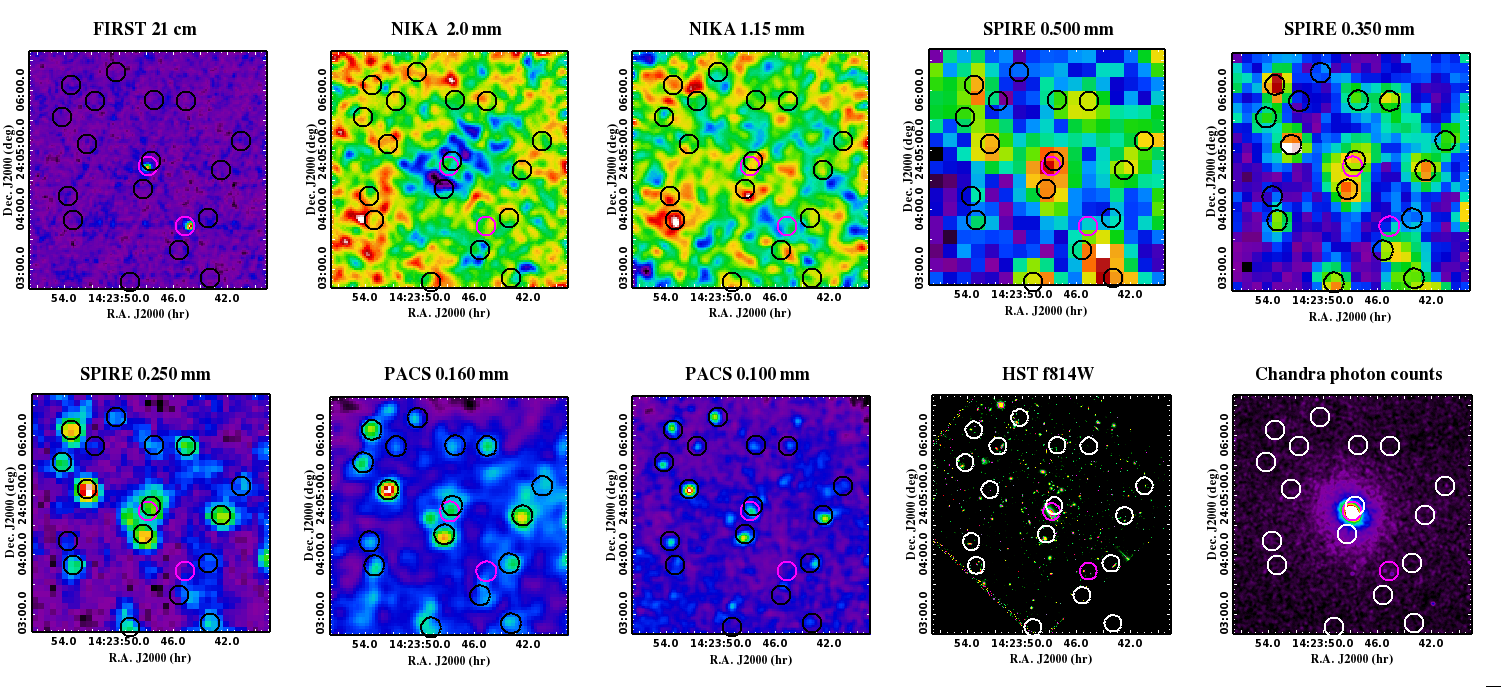
\includegraphics[trim=0cm 0cm 0cm 0cm, clip=true, width=0.99\textwidth]{Figure/MACSJ1424_multicolor.png}
\caption{\DIFaddbeginFL \footnotesize \DIFaddendFL Multi-wavelength dataset of \mbox{MACS~J1423.8+2404}. The origin of the data is given on top of each map. The maps have been smoothed and their range adapted for visualization purposes. The 10 arcsec radius circles \DIFdelbeginFL \DIFdelFL{give }\DIFdelendFL \DIFaddbeginFL \DIFaddFL{show }\DIFaddendFL the point \DIFdelbeginFL \DIFdelFL{sources }\DIFdelendFL \DIFaddbeginFL \DIFaddFL{source }\DIFaddendFL locations, in black/white for sub-millimeter sources (table~\ref{tab:IR_ps}) and magenta for radio sources (table~\ref{tab:Radio_ps}).}
\label{fig:MACSJ1424_mutiw2}
\end{figure*}

\DIFdelbegin \DIFdel{We give a multi-wavelength image of \mbox{MACS~J1423.8+2404} in }\DIFdelend Fig.~\ref{fig:MACSJ1424_mutiw} \DIFdelbegin \DIFdel{in order to directly compare the datasets. This provides a detailed picture }\DIFdelend \DIFaddbegin \DIFadd{shows a composite multi-wavelength image }\DIFaddend of the cluster\DIFdelbegin \DIFdel{ongoing physics and complements the discussion of Sect. ~\ref{sec:Introduction}. The figure represents }\DIFdelend \DIFaddbegin \DIFadd{. The figure includes }\DIFaddend the NIKA 150~GHz tSZ map, the Chandra X-ray photon counts, the NIKA and Herschel sub-millimeter galaxy locations, the NVSS radio \DIFdelbegin \DIFdel{sources }\DIFdelend \DIFaddbegin \DIFadd{source }\DIFaddend locations, and the HST image from CLASH. We also provide, for visual comparison, the surface mass distribution model of \mbox{MACS~J1423.8+2404} produced by \cite{zitrin2011} with the CLASH data. \DIFdelbegin %DIFDELCMD < 

%DIFDELCMD < %%%
\DIFdel{The }\DIFdelend \DIFaddbegin \DIFadd{The image provides a detailed picture of the cluster complements the discussion of Sect.~\ref{sec:Introduction}. The }\DIFaddend NIKA 150~GHz  \DIFdelbegin \DIFdel{detected tSZ signal is surrounding }\DIFdelend \DIFaddbegin \DIFadd{tSZ signal surrounds }\DIFaddend the cluster core. The hole seen in the tSZ signal is coincident with the BCG and results from the \DIFdelbegin \DIFdel{canceling }\DIFdelend \DIFaddbegin \DIFadd{cancelling }\DIFaddend of the tSZ by the radio and sub-millimeter signal, as discussed in Sect.~\ref{Radio_and_infrared_point_sources}. The X-ray morphology is very peaked and the maximum of \DIFaddbegin \DIFadd{the }\DIFaddend emission coincides with the BCG. The ellipticity of the spatial mass distribution is very clear from the strong lensing map. It is also visible in the X-ray map but is \DIFdelbegin \DIFdel{much }\DIFdelend less significant. It is not visible in the tSZ map due to the limited signal to noise and to the point source contamination\DIFdelbegin \DIFdel{which has not been removed at this stage}\DIFdelend . The galaxy distribution does not show any particular group that would be the sign of a merging event.
\DIFdelbegin %DIFDELCMD < \begin{figure}[h]
%DIFDELCMD < %%%
\DIFdelendFL \DIFaddbeginFL \begin{figure}[]
\DIFaddendFL \centering
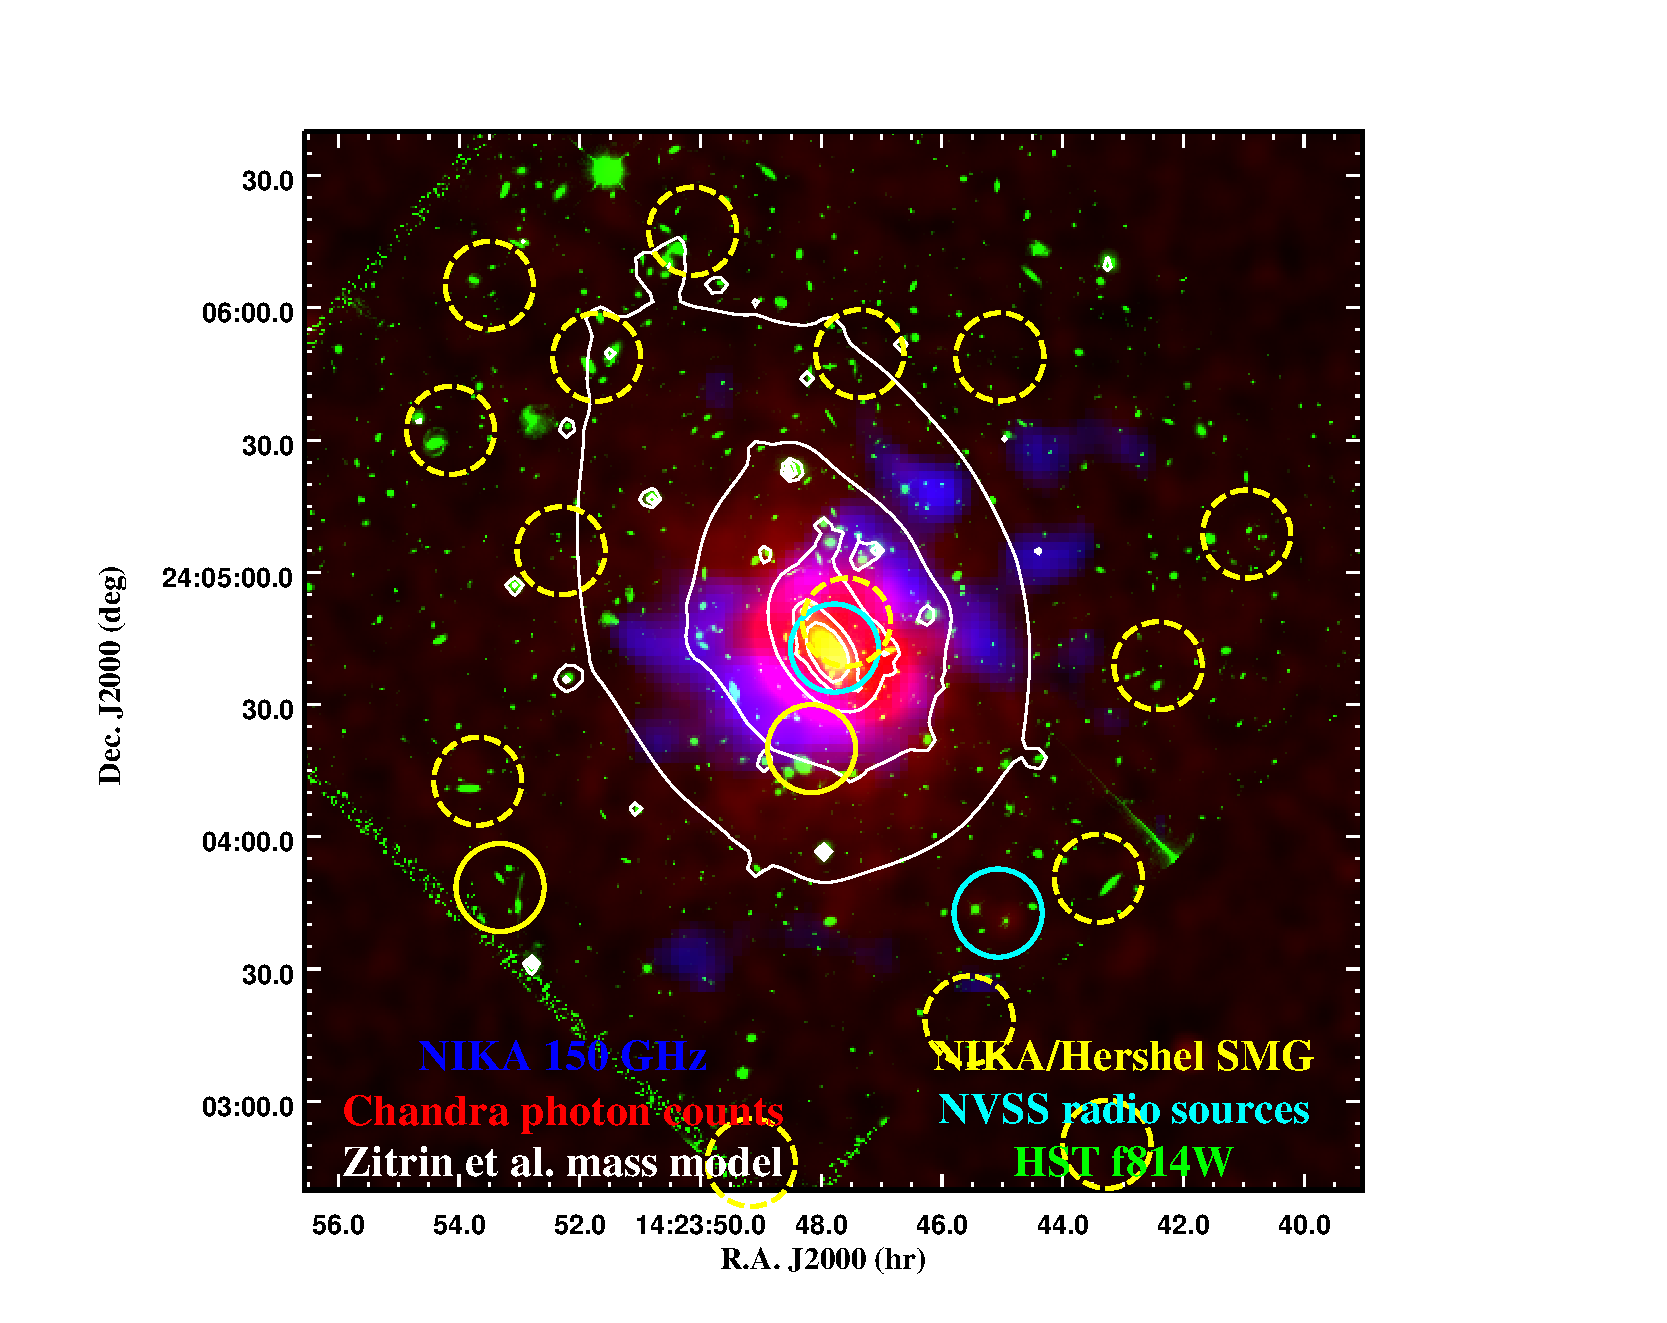
\includegraphics[trim=1cm 0cm 5cm 2cm, clip=true, width=0.45\textwidth]{Figure/MACSJ1424_multicolor.pdf}
\caption{\DIFaddbeginFL \footnotesize \DIFaddendFL Composite multi-wavelength \DIFaddbeginFL \DIFaddFL{overview }\DIFaddendFL image of \mbox{MACS~J1423.8+2404}. {\bf Blue image}: NIKA 150~GHz map showing the tSZ signal. {\bf Red image}: Chandra photon counts (Obs-ID 04195) tracing the electronic density. {\bf White contours}: surface mass distribution model obtained by \cite{zitrin2011} \DIFdelbeginFL \DIFdelFL{in }\DIFdelendFL \DIFaddbeginFL \DIFaddFL{on }\DIFaddendFL a linear scale. {\bf Yellow circles}: (sub-)millimeter sources candidate locations obtained using the NIKA 260~GHz map (solid line) and identified using Herschel (dashed-line). {\bf Cyan circle}: location of the radio point sources present in the field as obtained from VLA \citep{laroque2003}. {\bf Green image}: Hubble Space Telescope image using the F814W filter obtained by the CLASH  program \citep{postman2012} showing the location of \DIFdelbeginFL \DIFdelFL{optical }\DIFdelendFL \DIFaddbeginFL \DIFaddFL{the }\DIFaddendFL galaxies.}
\label{fig:MACSJ1424_mutiw}
\end{figure}

%###############################################################################################
%##########################                 PRESSURE RECONSTRUCTION                ##########################%###############################################################################################
\section{Radial thermodynamical reconstruction}\label{sec:Radial_pressure_reconstruction}
The radial physical properties of the ICM \DIFdelbegin \DIFdel{are }\DIFdelend \DIFaddbegin \DIFadd{were }\DIFaddend reconstructed using two approaches. The first\DIFdelbegin \DIFdel{one}\DIFdelend , detailed in Sect.~\ref{sec:X_ray_extraction_of_the_cluster_radial_thermodynamic_profiles}, uses \DIFaddbegin \DIFadd{the }\DIFaddend X-ray data only. The electronic density and the gas temperature are \DIFdelbegin \DIFdel{the primary quantities, which are }\DIFdelend directly measured and serve to reconstruct all the other \DIFdelbegin \DIFdel{ones}\DIFdelend \DIFaddbegin \DIFadd{quantities}\DIFaddend . This approach strongly depends on the spectroscopic temperature reconstruction. The second approach, detailed in Sect.~\ref{sec:modeling}, consists \DIFdelbegin \DIFdel{in }\DIFdelend \DIFaddbegin \DIFadd{of }\DIFaddend fitting jointly the tSZ data and the de-projected electronic density extracted from \DIFaddbegin \DIFadd{the }\DIFaddend X-ray data. The primary quantities are therefore the pressure and the electronic density, \DIFdelbegin \DIFdel{such that it }\DIFdelend \DIFaddbegin \DIFadd{and as such the method }\DIFaddend depends only weakly on X-ray spectroscopy, through the electronic density reconstruction. The comparison of the two approaches is given in Sect.~\ref{sec:results}.

%==========  Pressure profile estimation
\subsection{X-ray \DIFdelbegin \DIFdel{extraction of the cluster }\DIFdelend radial thermodynamic profiles}\label{sec:X_ray_extraction_of_the_cluster_radial_thermodynamic_profiles}
To compute the X-ray electronic pressure and entropy profiles we need to determine the temperature and electronic density profiles. \DIFdelbegin %DIFDELCMD < 

%DIFDELCMD < %%%
\DIFdel{The latter is computed by de-convolving and de-projecting the surface brightness profile using inversion with regularization as }\DIFdelend \DIFaddbegin \DIFadd{The latter was computed by applying the regularized deconvolution and deprojection technique }\DIFaddend described in \cite{croston2006}. We extracted the surface brightness profile from concentric annuli centered on the X-ray peak, (R.A., Dec.) = (14:23:47.9, +24:04:42.3), in the $[0.3-2.5] \ \si{\kilo\electronvolt}$ and $[0.7-2.5] \ \si{\kilo\electronvolt}$ \DIFdelbegin \DIFdel{band }\DIFdelend \DIFaddbegin \DIFadd{bands }\DIFaddend from the $3$ combined EPIC and ACIS cameras, respectively. \DIFdelbegin \DIFdel{The profiles after background subtraction}\DIFdelend \DIFaddbegin \DIFadd{After background subtraction, the profiles }\DIFaddend were re-binned by a logarithmic binning factor of $1.05$ to have a $3 \ \sigma$ significance for each bin, and were point spread function (PSF) de-convolved using the analytical model of \cite{ghizzardi2001} for XMM-Newton. For Chandra, we \DIFdelbegin \DIFdel{assume }\DIFdelend \DIFaddbegin \DIFadd{assumed }\DIFaddend that the PSF is negligible with respect to the \DIFdelbegin \DIFdel{widths }\DIFdelend \DIFaddbegin \DIFadd{width }\DIFaddend of the bins. 

The \DIFdelbegin \DIFdel{de-convolved and de-projected surface brightness profile }\DIFdelend \DIFaddbegin \DIFadd{deconvolved, deprojected surface brightness profiles }\DIFaddend were converted to \DIFdelbegin \DIFdel{a density profile }\DIFdelend \DIFaddbegin \DIFadd{density }\DIFaddend using a conversion factor determined from the projected temperature profile. \DIFdelbegin \DIFdel{To determine this profile we extracted }\DIFdelend \DIFaddbegin \DIFadd{The latter was determined by extracting }\DIFaddend spectra from concentric annuli centered on the X-ray peak, the width of each annulus being defined to have a signal to noise ratio of $30$ after background subtraction. We measured the temperature in each bin by fitting the spectrum with an absorbed \DIFdelbegin \DIFdel{MEKAL }\DIFdelend \DIFaddbegin {\sc \DIFadd{MEKAL}} \DIFaddend model, where the absorption \DIFdelbegin \DIFdel{is }\DIFdelend \DIFaddbegin \DIFadd{was }\DIFaddend fixed to $N_{H}=\SI{2.2e20}{\centi\meter}^{-3}$ \citep{kalberla2005}, \DIFaddbegin \DIFadd{the }\DIFaddend redshift to $z=0.545$, \DIFdelbegin \DIFdel{plus }\DIFdelend \DIFaddbegin \DIFadd{adding }\DIFaddend the scaled sky background component discussed above. To interpolate the temperature profile for each surface brightness bin, we fit \DIFdelbegin \DIFdel{to the observed temperature profile }\DIFdelend with the parametric model described in \cite{vikhlinin2006}. We note that the temperature correction is only a second order effect as the surface brightness is mainly dominated by the electronic density (see equation~\ref{eq:sx}). The differences in temperature reconstruction between Chandra and XMM-Newton \DIFaddbegin \DIFadd{\mbox{%DIFAUXCMD
\citep[e.g.,][]{sch15} }%DIFAUXCMD
thus }\DIFaddend do not affect the electronic density. \DIFdelbegin %DIFDELCMD < 

%DIFDELCMD < %%%
\DIFdelend To de-project the temperature profile, we measured the spectroscopic-like temperature \citep{mazzotta2004} using the weighting scheme implemented in \cite{vikh_multit}, where the observed temperature profile is modeled as the weighted sum of concentric plasma shells each at a different temperature. As for the density profiles, we take into account the PSF effects for XMM-Newton. 

Finally, $M_{500}$, the cluster mass enclosed within $R_{500}$\footnote{$R_{500}$ is the radius within which the mean cluster density is equal to 500 times the critical density of the Universe at the cluster's redshift.}, was calculated by iteration about the $M_{500}$--$Y_X$ relation of \cite{arnaud2010}.

%========== Modeling
\subsection{Modeling of the ICM and joint tSZ/X-ray fitting procedure}\label{sec:modeling}
%---------- What we do
To fit the tSZ and electronic density jointly, we \DIFdelbegin \DIFdel{model the cluster }\DIFdelend \DIFaddbegin \DIFadd{modeled the }\DIFaddend ICM using the \DIFdelbegin \DIFdel{same approach adopted for another NIKA cluster, described in details }\DIFdelend \DIFaddbegin \DIFadd{approach described }\DIFaddend in \DIFaddbegin \DIFadd{detail in }\DIFaddend \cite{adam2014}. As seen in Sect.~\ref{sec:Multi_wavelength_comparison} and \DIFaddbegin \DIFadd{as }\DIFaddend emphasized by \cite{morandi2010}, \mbox{MACS~J1423.8+2404} is elliptical. Nevertheless, we assume spherical symmetry because this work does not focus on its geometry, but on the impact of the presence of point sources on the pressure profile reconstruction. Moreover, the significance of the NIKA 150~GHz tSZ map is not sufficient to constrain \DIFdelbegin \DIFdel{this asymmetry. 
We summarize here the procedure adopted to recover the cluster radial physical properties.
}\DIFdelend \DIFaddbegin \DIFadd{any asymmetry. 
}\DIFaddend 

%---------- Model
The radial distribution of the cluster electronic pressure \DIFdelbegin \DIFdel{is }\DIFdelend \DIFaddbegin \DIFadd{was }\DIFaddend modeled by a gNFW profile \citep{nagai2007}, described by
\begin{equation}
	P_e(r) = \frac{P_0}{\left(\frac{r}{r_p}\right)^c \left(1+\left(\frac{r}{r_p}\right)^a\right)^{\frac{b-c}{a}}}.
\label{eq:gNFW}
\end{equation}
The parameter $P_0$ is a normalization constant; $r_p$ is a characteristic radius; and $a$, $b$, and $c$ set the slopes at intermediate, large, and small radii, respectively. This model \DIFdelbegin \DIFdel{is }\DIFdelend \DIFaddbegin \DIFadd{was }\DIFaddend chosen to allow the description of the profile at all scales. The electronic density \DIFdelbegin \DIFdel{is }\DIFdelend \DIFaddbegin \DIFadd{was }\DIFaddend modeled by a \emph{Simplified Vikhlinin Model} \citep{vikhlinin2006},
\begin{equation}
	n_e(r) = n_{e0} \left[1+\left(\frac{r}{r_c}\right)^2 \right]^{-3 \beta /2} \left[ 1+\left(\frac{r}{r_s}\right)^{\gamma} \right]^{-\epsilon/2 \gamma}.
\label{eq:SVM}
\end{equation}
The parameter $n_{e0}$ is the central density, $r_c$ is the core radius and $\beta$ is related to the slope of the profile. The second term allows \DIFdelbegin \DIFdel{the description }\DIFdelend \DIFaddbegin \DIFadd{a }\DIFaddend of the steepening of the profile at large scales. The parameter $\epsilon$ gives the change in the slope, $r_s$ the radius at which the transition occurs, and $\gamma$ the width of the transition. In the following, we set $\gamma = 3$ since \DIFdelbegin \DIFdel{it }\DIFdelend \DIFaddbegin \DIFadd{this value }\DIFaddend provides a good fit to all clusters considered in the analysis of \cite{vikhlinin2006}.

With the pressure and the density in hand, we compute the temperature profile assuming the ideal gas law, $k_B T_e(r) = \frac{P_e(r)}{n_e(r)}$, and the entropy profile as $K(r) =  \frac{P_e(r)}{n_e(r)^{5/3}}$\DIFdelbegin \DIFdel{following \mbox{%DIFAUXCMD
\cite{voit2005}}%DIFAUXCMD
}\DIFdelend . The total mass, assuming hydrostatic equilibrium, enclosed within $r$ is then given by 
\DIFdelbegin \DIFdel{$M_{\rm HSE}(r) = -\frac{r^2}{\mu_{gas} m_p n_e(r) G} \frac{dP_e(r)}{dr}$, }\DIFdelend \DIFaddbegin \begin{equation}
\DIFadd{M_{\rm HSE}(r) = -\frac{r^2}{\mu_{gas} m_p n_e(r) G} \frac{dP_e(r)}{dr}
}\end{equation}
\DIFaddend where $m_p$ is the proton mass, $G$ \DIFdelbegin \DIFdel{the }\DIFdelend \DIFaddbegin \DIFadd{is }\DIFaddend Newton’s constant, and $\mu_{gas} = 0.61$ the mean molecular weight of the gas.

%---------- Fit
The parameter space \DIFdelbegin \DIFdel{is }\DIFdelend \DIFaddbegin \DIFadd{was }\DIFaddend sampled using the Markov Chain Monte Carlo \DIFaddbegin \DIFadd{(MCMC) }\DIFaddend approach detailed in \cite{adam2014}\DIFdelbegin \DIFdel{. We jointly fit }\DIFdelend \DIFaddbegin \DIFadd{, jointly fitting }\DIFaddend the 150~GHz NIKA tSZ map \DIFdelbegin \DIFdel{, }\DIFdelend \DIFaddbegin \DIFadd{and }\DIFaddend the electronic density profile computed from the \DIFdelbegin \DIFdel{deprojection of the }\DIFdelend X-ray data. \DIFdelbegin \DIFdel{In addition, we add a }\DIFdelend \DIFaddbegin \DIFadd{We added an additional }\DIFaddend constraint on the total tSZ flux of the cluster using the Planck Compton parameter map \citep{planck2015XXII}. The tSZ models \DIFdelbegin \DIFdel{are }\DIFdelend \DIFaddbegin \DIFadd{were }\DIFaddend convolved with the effective transfer function of the observations, including the beam smoothing and the large scale filtering cutoff due to the removal of the atmospheric noise. \DIFdelbegin \DIFdel{The cluster }\DIFdelend \mbox{MACS~J1423.8+2404} is not present in the Planck catalogue of tSZ sources \citep{planck2015XXVII}, but we \DIFdelbegin \DIFdel{obtain an upper bound }\DIFdelend \DIFaddbegin \DIFadd{obtained an upper limit }\DIFaddend on its flux by integrating the Compton parameter map \citep{planck2015XXII} using aperture photometry. The error on the flux \DIFdelbegin \DIFdel{is }\DIFdelend \DIFaddbegin \DIFadd{was }\DIFaddend computed by performing the same measurement randomly around the cluster, where the noise is homogeneous. The flux \DIFdelbegin \DIFdel{is }\DIFdelend \DIFaddbegin \DIFadd{was }\DIFaddend measured to be $Y_{\rm tot}^{\rm Planck} = \left(0.40 \pm 0.66\right) \times 10^{-3}$ arcmin$^2$. \DIFdelbegin \DIFdel{During the MCMC sampling , we also marginalize }\DIFdelend \DIFaddbegin \DIFadd{The MCMC sampling procedure also marginalizes }\DIFaddend over nuisance parameters such as the zero level of the NIKA map, the calibration uncertainty, \DIFdelbegin \DIFdel{or }\DIFdelend \DIFaddbegin \DIFadd{and }\DIFaddend the central point source flux and position when included in the fit. \DIFdelbegin \DIFdel{See \mbox{%DIFAUXCMD
\cite{adam2014} }%DIFAUXCMD
for more details }\DIFdelend \DIFaddbegin \DIFadd{Full details can be found in \mbox{%DIFAUXCMD
\cite{adam2014}}%DIFAUXCMD
}\DIFaddend .

%---------- Where does the constraints come from
The constraints obtained on the pressure and electronic density profiles are almost independent. \DIFdelbegin \DIFdel{Nevertheless}\DIFdelend \DIFaddbegin \DIFadd{However}\DIFaddend , each model compared to the data \DIFdelbegin \DIFdel{include }\DIFdelend \DIFaddbegin \DIFadd{includes }\DIFaddend relativistic corrections computed using the radial temperature profile, given by the ratio of the electronic pressure and density profiles, for each radial shell of the ICM. This affects essentially the constraint on the pressure profile but \DIFdelbegin \DIFdel{this }\DIFdelend \DIFaddbegin \DIFadd{the }\DIFaddend effect is very small compared to the \DIFdelbegin \DIFdel{error bars}\DIFdelend \DIFaddbegin \DIFadd{uncertainties}\DIFaddend . Therefore, the constraint on the electronic density profile is \DIFdelbegin \DIFdel{provided }\DIFdelend \DIFaddbegin \DIFadd{driven }\DIFaddend by the X-ray data and that \DIFdelbegin \DIFdel{of the electronic }\DIFdelend \DIFaddbegin \DIFadd{on the }\DIFaddend pressure is largely driven by the tSZ data. \DIFdelbegin \DIFdel{In the case of \mbox{MACS~J1423.8+2404}, the }\DIFdelend \DIFaddbegin \DIFadd{The }\DIFaddend Planck constraint on the overall tSZ flux is relatively weak due to the location of the cluster on the sky and \DIFaddbegin \DIFadd{the }\DIFaddend noise inhomogeneity. However, Planck provides an upper limit that allows \DIFaddbegin \DIFadd{the MCMC procedure }\DIFaddend to avoid models which diverge at large scales, where NIKA is not sensitive. Planck and NIKA are therefore highly complementary to constrain the pressure profile from small to large scales.

%========== Results
\subsection{Results}\label{sec:results}
\DIFdelbegin \DIFdel{The cluster }\DIFdelend \mbox{MACS~J1423.8+2404} is known to be a typical cool core \citep[e.g.][]{morandi2010}\DIFdelbegin \DIFdel{. Therefore, we use as a baseline }\DIFdelend \DIFaddbegin \DIFadd{, so we used }\DIFaddend the pressure profile \DIFdelbegin \DIFdel{slopes }\DIFdelend \DIFaddbegin \DIFadd{parameters }\DIFaddend found for such clusters by \cite{arnaud2010} \DIFaddbegin \DIFadd{as a baseline}\DIFaddend : $\left(a,b,c\right) = \left(1.2223, 5.4905, 0.7736\right)$. The X-ray photon count provided by XMM-Newton is larger than that of Chandra, allowing \DIFaddbegin \DIFadd{us }\DIFaddend to probe the cluster ICM up to larger radii\DIFdelbegin \DIFdel{, especially in terms of temperature, pressure, and entropy. This is why, in the present work, }\DIFdelend \DIFaddbegin \DIFadd{. We therefore used the }\DIFaddend XMM-Newton \DIFdelbegin \DIFdel{is used }\DIFdelend \DIFaddbegin \DIFadd{results }\DIFaddend as a reference and we \DIFdelbegin \DIFdel{cross-check }\DIFdelend \DIFaddbegin \DIFadd{cross-checked }\DIFaddend our results with \DIFaddbegin \DIFadd{the }\DIFaddend Chandra data.

%++++++++++ Test of the point sources
\subsubsection{Impact of the point sources at millimeter \DIFdelbegin \DIFdel{wavelength}\DIFdelend \DIFaddbegin \DIFadd{wavelengths}\DIFaddend }
%---------- How to test point impact of sources
The impact of the point source contamination on the reconstructed pressure profile \DIFdelbegin \DIFdel{is }\DIFdelend \DIFaddbegin \DIFadd{was }\DIFaddend tested by considering three different cases: 
\begin{enumerate}
\item The presence of point sources \DIFdelbegin \DIFdel{is }\DIFdelend \DIFaddbegin \DIFadd{was }\DIFaddend ignored and we fit the parameters $P_0$ and $r_p$, keeping the slope parameters fixed to their baseline values. This case is referred as model 1 (M1).
\item The point sources \DIFdelbegin \DIFdel{are }\DIFdelend \DIFaddbegin \DIFadd{were }\DIFaddend subtracted assuming the fluxes of Table \ref{tab:IR_ps2} and we \DIFdelbegin \DIFdel{repeat }\DIFdelend \DIFaddbegin \DIFadd{repeated }\DIFaddend the fit of model M1. This case is referred as model 2 (M2).
\item The point sources \DIFdelbegin \DIFdel{are }\DIFdelend \DIFaddbegin \DIFadd{were }\DIFaddend subtracted assuming the fluxes \DIFdelbegin \DIFdel{of }\DIFdelend \DIFaddbegin \DIFadd{given in }\DIFaddend Table \ref{tab:IR_ps2}, but possible residuals of the central sources \DIFdelbegin \DIFdel{are }\DIFdelend \DIFaddbegin \DIFadd{were }\DIFaddend also fitted. In this case, we also \DIFdelbegin \DIFdel{release }\DIFdelend \DIFaddbegin \DIFadd{released }\DIFaddend the constraint on the inner and outer slope parameters, $c$ and $b$, which are also fitted. The intermediate slope parameter $a$ \DIFdelbegin \DIFdel{is }\DIFdelend \DIFaddbegin \DIFadd{was }\DIFaddend held fixed because it is strongly \DIFdelbegin \DIFdel{degenerated }\DIFdelend \DIFaddbegin \DIFadd{degenerate }\DIFaddend with the characteristic radius $r_p$ and the outer slope $b$. This case is referred as model 3 (M3).
\end{enumerate}
\DIFdelbegin \DIFdel{The comparison }\DIFdelend \DIFaddbegin \DIFadd{Comparison }\DIFaddend of the output pressure profile \DIFdelbegin \DIFdel{of }\DIFdelend \DIFaddbegin \DIFadd{from }\DIFaddend models M1 and M2 (see Fig.~\ref{fig:MACSJ1424_pressure_point_source}) allows a direct estimation of the impact of point sources. The use of model M3 \DIFdelbegin \DIFdel{is }\DIFdelend \DIFaddbegin \DIFadd{was }\DIFaddend motivated by the large uncertainties on the point source fluxes as shown in Table \ref{tab:IR_ps2}. As discussed in Sect.~\ref{sec:surface_brightness_profiles_comparison} and shown on Fig.~\ref{fig:flux_profiles}, the sources that are in the outer region of the cluster do not contribute significantly to the radial flux density. However, this is not the case for the central sources, in particular for RS1 and SMG05. We expect a significant correlation between the flux of these sources and the pressure profile parameters related to the cluster core, such as $P_0$, $r_p$ and $c$. Those related to the external regions of the profile are also affected, due to projection effects. \DIFdelbegin \DIFdel{Therefore, }\DIFdelend \DIFaddbegin \DIFadd{Thus }\DIFaddend model M3 allows \DIFaddbegin \DIFadd{us }\DIFaddend to test the constraints that can be obtained on the pressure profile \DIFdelbegin \DIFdel{at }\DIFdelend \DIFaddbegin \DIFadd{in }\DIFaddend the cluster core in \DIFaddbegin \DIFadd{the }\DIFaddend presence of a contaminating central point source, when no strong prior on its flux is available, as \DIFdelbegin \DIFdel{it }\DIFdelend is the case here.

%---------- Results on the constrained profile
\DIFdelbegin \DIFdel{The pressure profile measured in the three cases is given in Fig.~\ref{fig:MACSJ1424_pressure_point_source} }\DIFdelend \DIFaddbegin \DIFadd{Figure~\ref{fig:MACSJ1424_pressure_point_source} shows the resulting pressure profiles}\DIFaddend . Model M1 is lower than the two \DIFdelbegin \DIFdel{other }\DIFdelend \DIFaddbegin \DIFadd{others }\DIFaddend at all scales \DIFdelbegin \DIFdel{, }\DIFdelend except above 1000 kpc\DIFaddbegin \DIFadd{, }\DIFaddend where NIKA does not provide a direct constraint \DIFdelbegin \DIFdel{, }\DIFdelend due to the large \DIFdelbegin \DIFdel{scales }\DIFdelend \DIFaddbegin \DIFadd{scale }\DIFaddend filtering. This corresponds to the fact that point sources, and in particular those close to the core, compensate the overall flux amplitude of the cluster. Apart from its normalization, the shape of the pressure profile is similar for M1 and M2 as the constraint on $r_p$ is not significantly affected by the point \DIFdelbegin \DIFdel{sources }\DIFdelend \DIFaddbegin \DIFadd{source }\DIFaddend subtraction. The effect of the source in the cluster core is then diluted over \DIFdelbegin \DIFdel{all the }\DIFdelend \DIFaddbegin \DIFadd{the entire  }\DIFaddend profile via the $P_0$ -- $r_p$ degeneracy. The results for M3 are close to those \DIFdelbegin \DIFdel{of }\DIFdelend \DIFaddbegin \DIFadd{for }\DIFaddend M2 but \DIFaddbegin \DIFadd{the }\DIFaddend error contours are larger because of the extra freedom available in the parameter space. This is particularly true in the inner region, where the error on the flux of the fitted point source propagates \DIFdelbegin \DIFdel{to }\DIFdelend \DIFaddbegin \DIFadd{into }\DIFaddend the profile via the \DIFdelbegin \DIFdel{degeneracies between parameters. Therefore, the }\DIFdelend \DIFaddbegin \DIFadd{parameter degeneracies. The }\DIFaddend inner pressure distribution \DIFdelbegin \DIFdel{remains unconstrained }\DIFdelend \DIFaddbegin \DIFadd{thus remains poorly constrained }\DIFaddend unless the point \DIFdelbegin \DIFdel{sources }\DIFdelend \DIFaddbegin \DIFadd{source }\DIFaddend is subtracted with sufficient accuracy. At large scales, around 800 kpc,  \DIFdelbegin \DIFdel{the best-fit model }\DIFdelend M3 is slightly above \DIFdelbegin \DIFdel{the }\DIFdelend M2\DIFdelbegin \DIFdel{one}\DIFdelend . However, \DIFdelbegin \DIFdel{it is important to notice that }\DIFdelend the differences observed between models are not significant with respect to the uncertainties, which are dominated by the low exposure time spent with NIKA on this cluster.
\begin{figure}[h]
\centering
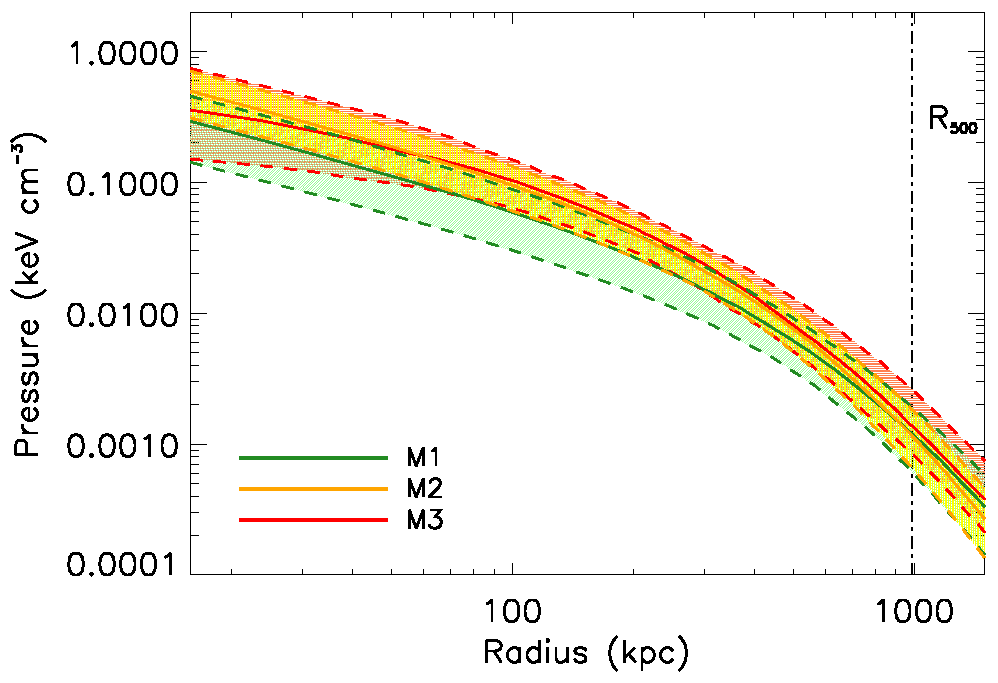
\includegraphics[width=0.49\textwidth]{Figure/ICM_pressure_profile_point_sources.pdf}
\caption{\DIFaddbeginFL \footnotesize \DIFaddendFL Constraint on the pressure profile of \mbox{MACS~J1423.8+2404} for the three models M1 (green), M2 (orange) and M3 (red). The solid lines gives the central profiles and the dashed line represent the 68\% confidence limits.}
\label{fig:MACSJ1424_pressure_point_source}
\end{figure}

%---------- Morphology
To search for possible deviations from \DIFdelbegin \DIFdel{the }\DIFdelend \DIFaddbegin \DIFadd{a }\DIFaddend spherical relaxed morphology, \DIFdelbegin \DIFdel{as expected according to X-ray and lensing observations, }\DIFdelend \DIFaddbegin \DIFadd{we subtracted }\DIFaddend the best-fit model of M3 \DIFdelbegin \DIFdel{is subtracted }\DIFdelend from the NIKA 150~GHz map. Fig.~\ref{fig:MACSJ1424_MCMC_modeling} \DIFdelbegin \DIFdel{represents the }\DIFdelend \DIFaddbegin \DIFadd{shows the resulting }\DIFaddend raw, point \DIFdelbegin \DIFdel{sources }\DIFdelend \DIFaddbegin \DIFadd{source }\DIFaddend subtracted, tSZ best-fit, and residual 150~GHz maps. After removing the point sources (fluxes in Table \ref{tab:IR_ps2}) and the best-fit of model M3, the cluster appears to be fairly compact\DIFdelbegin \DIFdel{with a }\DIFdelend \DIFaddbegin \DIFadd{. The }\DIFaddend small excess towards the south \DIFdelbegin \DIFdel{. However, the significance of the latter is }\DIFdelend \DIFaddbegin \DIFadd{has a significance of }\DIFaddend less than 2 $\sigma$ and can be attributed to a poor subtraction of SMG05, whose position is very close on the map. The signal is \DIFdelbegin \DIFdel{on }\DIFdelend overall relatively spherical, as confirmed by the residual \DIFaddbegin \DIFadd{map, }\DIFaddend which is consistent with the noise. Deeper tSZ observations would be necessary in order to further constrain the morphology of the cluster, in particular in terms of ellipticity.
\begin{figure*}[h]
\centering
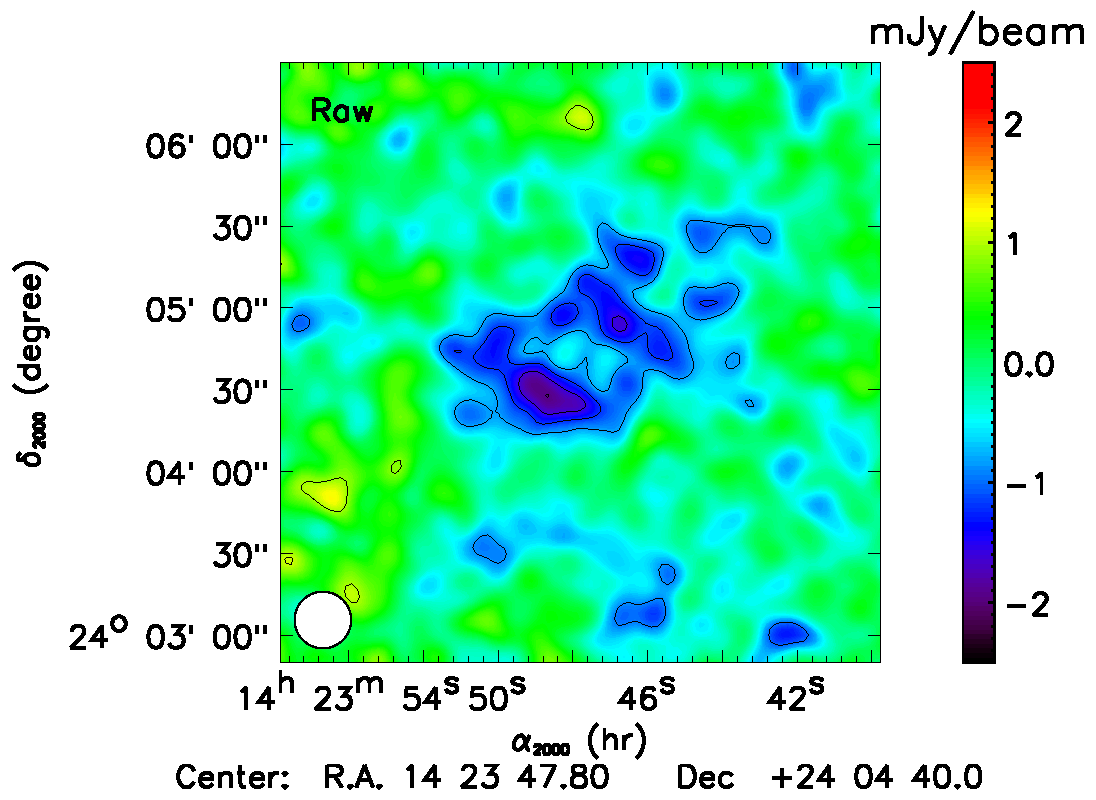
\includegraphics[width=0.49\textwidth]{Figure/MCMC_raw_map.pdf}
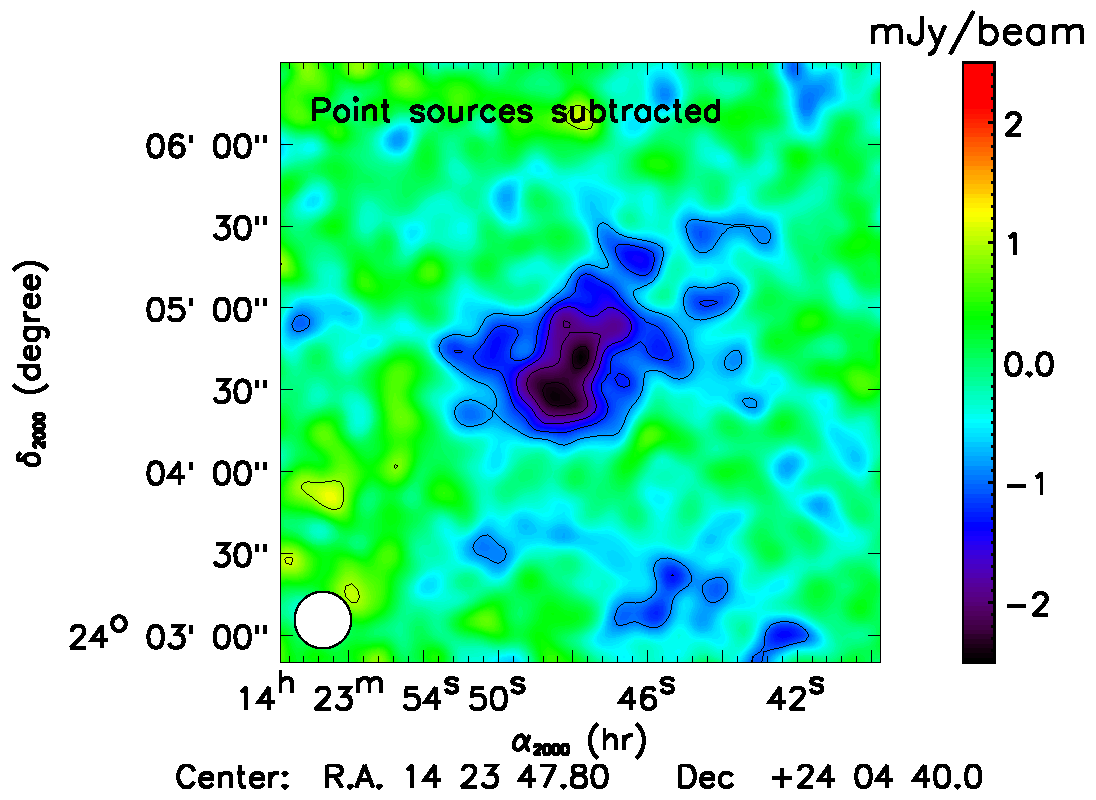
\includegraphics[width=0.49\textwidth]{Figure/MCMC_point_source_removed.pdf}
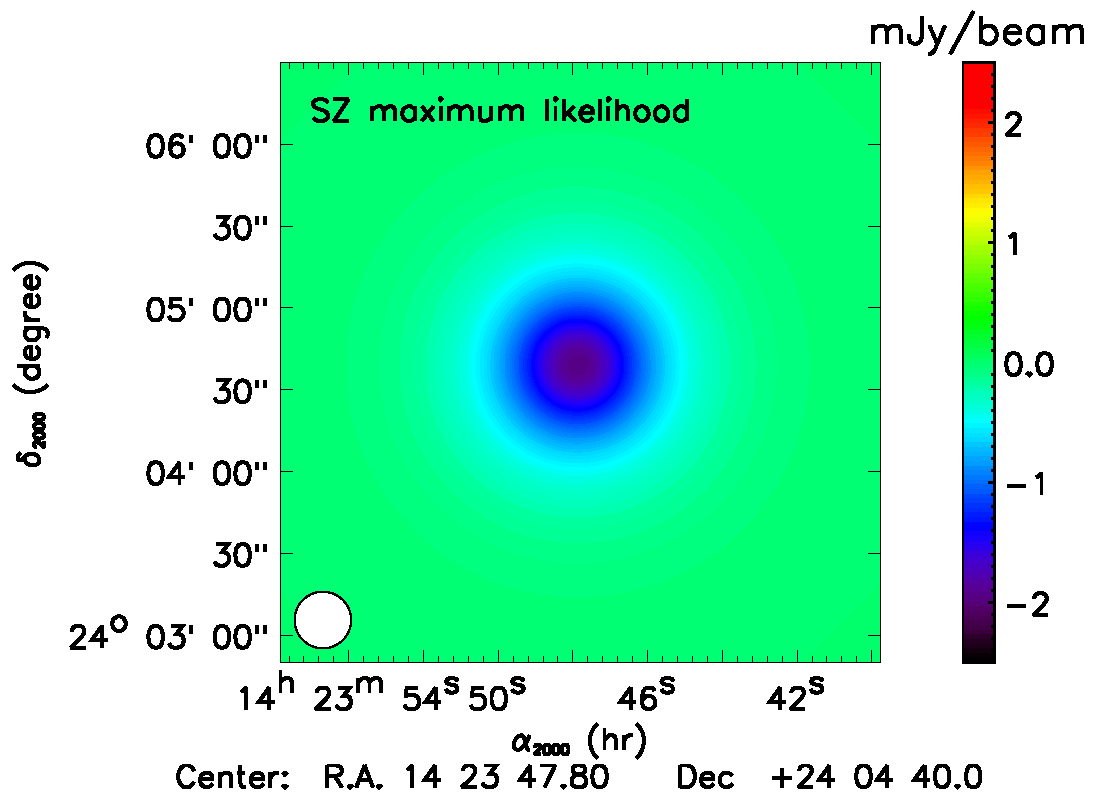
\includegraphics[width=0.49\textwidth]{Figure/MCMC_best_fit.pdf}
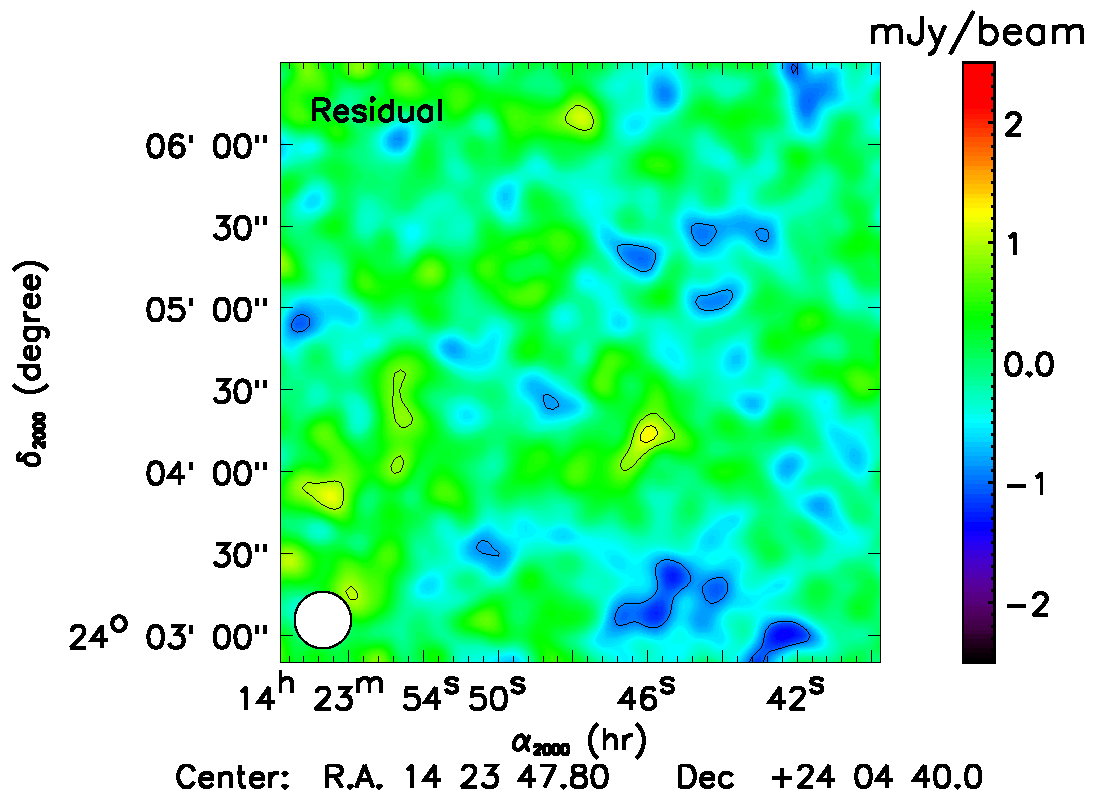
\includegraphics[width=0.49\textwidth]{Figure/MCMC_residual.pdf}
\caption{\DIFaddbeginFL \footnotesize \DIFaddendFL Comparison of the raw 150~GHz input NIKA map (top left), the same map after point \DIFdelbeginFL \DIFdelFL{sources }\DIFdelendFL \DIFaddbeginFL \DIFaddFL{source }\DIFaddendFL subtraction (top right), the best-fit tSZ model (bottom left), and the final residual map. Contours are the same as in Fig.~\ref{fig:flux_map} \DIFdelbeginFL \DIFdelFL{, they }\DIFdelendFL \DIFaddbeginFL \DIFaddFL{and }\DIFaddendFL give the significance in unit of $\sigma$, starting from $\pm 2 \ \sigma$. \DIFdelbeginFL \DIFdelFL{Uncertainties arising from the point sources and the model subtraction are ignored on these contours.}\DIFdelendFL }
\label{fig:MACSJ1424_MCMC_modeling}
\end{figure*}

%++++++++++ X vs tSZ
\subsubsection{Comparison between tSZ and X-ray derived cluster thermodynamics}
%---------- Flux density profile and X-ray density
Fig.~\ref{fig:MACSJ1424_MCMC_vs_data} \DIFdelbegin \DIFdel{provides }\DIFdelend \DIFaddbegin \DIFadd{shows }\DIFaddend a comparison of the MCMC constraints and the data used to obtain them. The left panel presents the best-fit and the uncertainties of model M3 \DIFdelbegin \DIFdel{on }\DIFdelend \DIFaddbegin \DIFadd{compared to }\DIFaddend the projected flux density profile \DIFdelbegin \DIFdel{, and compares it with the NIKA data, subtracted }\DIFdelend from the point \DIFdelbegin \DIFdel{sources based on Table \ref{tab:IR_ps2}}\DIFdelend \DIFaddbegin \DIFadd{source-subtracted NIKA data}\DIFaddend . The data points are correlated across the profile and we \DIFdelbegin \DIFdel{account }\DIFdelend \DIFaddbegin \DIFadd{accounted }\DIFaddend for this in the MCMC analysis. The \DIFaddbegin \DIFadd{model }\DIFaddend uncertainties increase significantly in the cluster core because the flux estimate (and associated uncertainty) of the central point source is included in the fit. The model is greater than zero at large scales because the zero level of the map (one of the nuisance parameters included in the fit) is slightly positive. The right panel \DIFdelbegin \DIFdel{provides }\DIFdelend \DIFaddbegin \DIFadd{shows }\DIFaddend the best-fit to the XMM-Newton electronic density and its \DIFdelbegin \DIFdel{uncertainty at }\DIFdelend 68\% confidence limit. We also \DIFdelbegin \DIFdel{represent }\DIFdelend \DIFaddbegin \DIFadd{show }\DIFaddend the Chandra data for comparison. The \DIFdelbegin \DIFdel{XMM-Newton }\DIFdelend \DIFaddbegin \DIFadd{X-ray }\DIFaddend data are well described by the SVM model, except at radii smaller than 30 kpc, where we observe a flattening of the data with respect to the model. However, this region is not probed directly by NIKA and this deviation is not significant in the context of the joint tSZ/X-ray analysis.
\begin{figure*}[h]
\centering
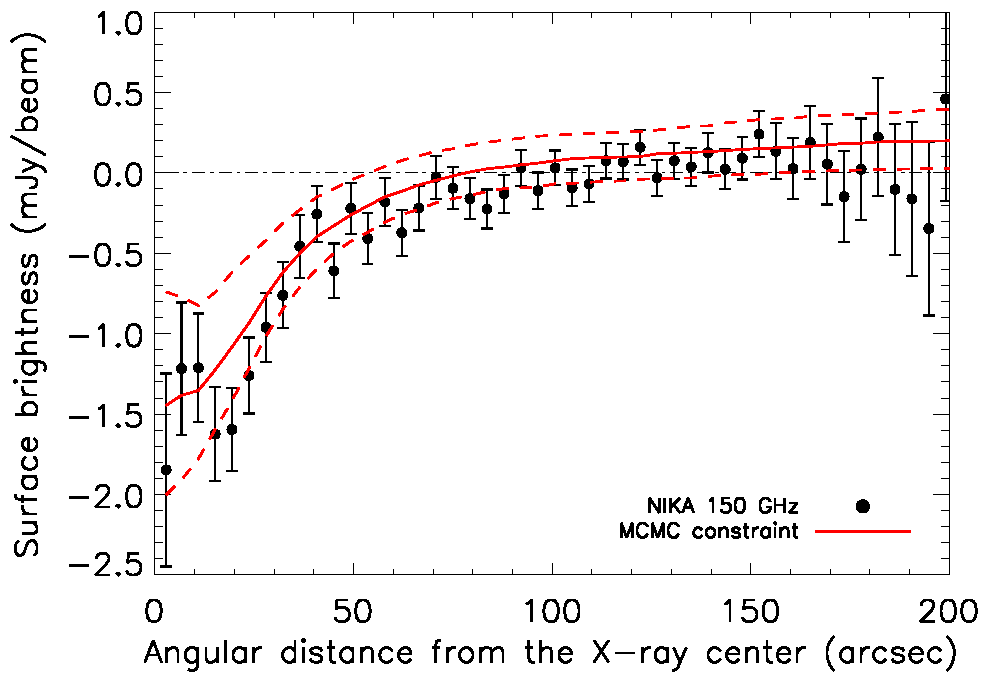
\includegraphics[height=6.3cm]{Figure/MACSJ1424_profile_ML.pdf}
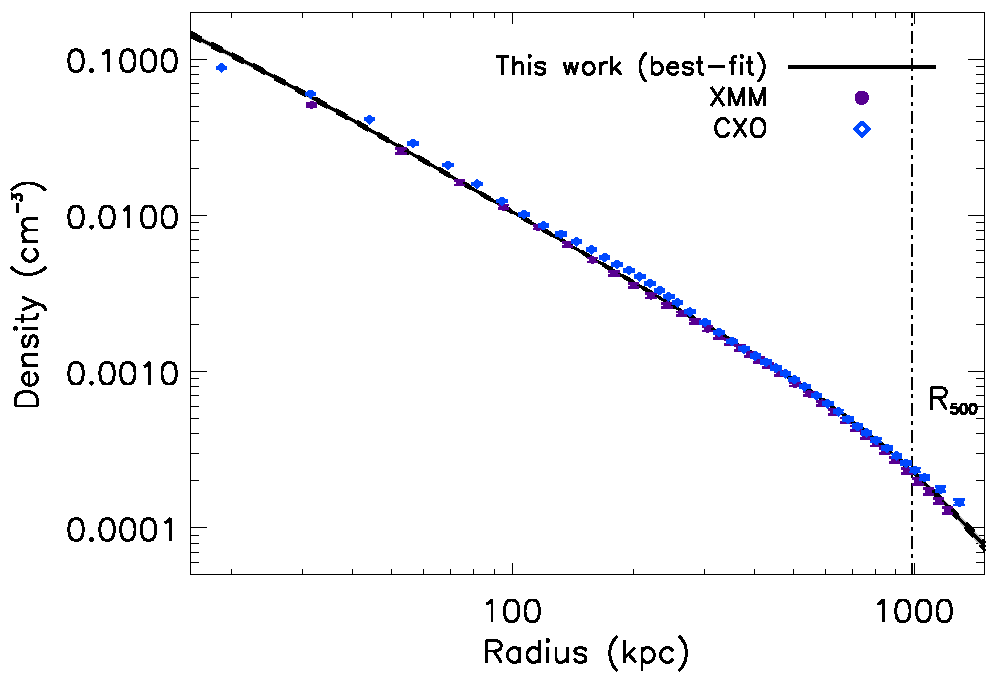
\includegraphics[height=6.3cm]{Figure/ICM_density_profile.pdf}
\caption{\DIFaddbeginFL \footnotesize \DIFaddendFL MCMC best-fit and constraints compared to the NIKA tSZ and XMM-Newton X-ray data used to obtain them. {\bf Left}: projected tSZ flux density profile \DIFdelbeginFL \DIFdelFL{for }\DIFdelendFL \DIFaddbeginFL \DIFaddFL{from }\DIFaddendFL the point \DIFdelbeginFL \DIFdelFL{sources }\DIFdelendFL \DIFaddbeginFL \DIFaddFL{source }\DIFaddendFL subtracted NIKA data (black dots) and for the \DIFdelbeginFL \DIFdelFL{M3 }\DIFdelendFL best-fit \DIFaddbeginFL \DIFaddFL{M3 }\DIFaddendFL model (red solid line). Uncertainties at 68\% confidence limits are given by the red dashed lines. We note that, in practice, it is the tSZ map which is compared to the models and not the profile. {\bf Right}: deprojected electronic density profile obtained from XMM-Newton (purple dots) and Chandra (CXO for Chandra X-ray Observatory, blue diamonds). The MCMC best-fit model is given by the black line\DIFaddbeginFL \DIFaddFL{, }\DIFaddendFL and its uncertainties at 68\% confidence limits are shown by the black dashed lines. The characteristic radius measured from XMM-Newton data, $R_{500} = 986 \pm 10$ kpc, is represented as a vertical dashed line.}
\label{fig:MACSJ1424_MCMC_vs_data}
\end{figure*}

%---------- Pressure profile
The top left panel of Fig.~\ref{fig:MACSJ1424_MCMC_tk_profile} shows the deprojected pressure profile of \mbox{MACS~J1423.8+2404} as derived from our MCMC analysis \DIFaddbegin \DIFadd{of NIKA data, }\DIFaddend and from X-ray \DIFdelbegin \DIFdel{measurement }\DIFdelend \DIFaddbegin \DIFadd{measurements }\DIFaddend only. While deep X-ray observations can only infer the pressure (using the product of the de-projected density and temperature profiles), the tSZ effect directly measures it. The comparison of the two, which are completely independent, is therefore an important cross check for both constraints. The data points represent measurements obtained from XMM-Newton and Chandra, and the shaded area is the 68\% confidence limit given by model M2. The upper and lower dashed lines give respectively the upper and lower limits from all the tSZ based models M1, M2 and M3. The Chandra constraint is slightly more peaked than \DIFdelbegin \DIFdel{the }\DIFdelend \DIFaddbegin \DIFadd{that from }\DIFaddend XMM-Newton\DIFdelbegin \DIFdel{one}\DIFdelend . In turn, the latter is slightly more peaked than \DIFdelbegin \DIFdel{the tSZ one}\DIFdelend \DIFaddbegin \DIFadd{that from NIKA}\DIFaddend , but all \DIFdelbegin \DIFdel{of them }\DIFdelend \DIFaddbegin \DIFadd{profiles }\DIFaddend are compatible within error bars. These results confirm that the point spread function deconvolution of the XMM-Newton data performs well and that the model extrapolation of the tSZ data accurately describes the pressure profile at the cluster center. At large radii, the Chandra measurement is not available due to a \DIFaddbegin \DIFadd{lower }\DIFaddend photon count rate  \DIFdelbegin \DIFdel{lower }\DIFdelend than XMM-Newton\DIFaddbegin \DIFadd{, }\DIFaddend making the two observations \DIFaddbegin \DIFadd{highly }\DIFaddend complementary. The tSZ  \DIFdelbegin \DIFdel{measured }\DIFdelend pressure profile decreases slightly \DIFdelbegin \DIFdel{slower than }\DIFdelend \DIFaddbegin \DIFadd{more slowly than that from XMM-Newton, but }\DIFaddend the \DIFdelbegin \DIFdel{X-ray one but this }\DIFdelend effect is not significant with respect to the uncertainties. 

We \DIFdelbegin \DIFdel{compare }\DIFdelend \DIFaddbegin \DIFadd{compared }\DIFaddend our measurements to the universal pressure profile \DIFdelbegin \DIFdel{measured by \mbox{%DIFAUXCMD
\cite{arnaud2010} }%DIFAUXCMD
from REXCESS }\DIFdelend \DIFaddbegin \DIFadd{obtained by \mbox{%DIFAUXCMD
\cite{arnaud2010} }%DIFAUXCMD
using  }\rexcess\DIFadd{\  }\DIFaddend \citep{bohringer2007}, a representative sample of nearby clusters. The green and orange solid lines \DIFdelbegin \DIFdel{provide the expected }\DIFdelend \DIFaddbegin \DIFadd{show the mean }\DIFaddend profiles for the cool core and morphologically disturbed sub-samples used by \cite{arnaud2010}, respectively. The normalization (\DIFdelbegin \DIFdel{see equation }\DIFdelend \DIFaddbegin \DIFadd{eqn.~}\DIFaddend 13 of \cite{arnaud2010}) was accounted for using the XMM-Newton mass measurement of \mbox{MACS~J1423.8+2404}, and neglecting the mass dependance of the shape of the profile. \DIFdelbegin \DIFdel{We can observe that }\DIFdelend \DIFaddbegin \DIFadd{The observed pressure distribution of  }\DIFaddend \mbox{MACS~J1423.8+2404} compares well to the \DIFdelbegin \DIFdel{cool core expectation }\DIFdelend \DIFaddbegin \DIFadd{mean cool core profile }\DIFaddend both in shape and amplitude. The \DIFdelbegin \DIFdel{profile associated to morphologically disturbed clusters }\DIFdelend \DIFaddbegin \DIFadd{mean morphologically disturbed profile }\DIFaddend is consistent with the observations at large scales, but deviates significantly in the core, being much shallower than the observations because of the redistribution of the thermal energy from merging events in such clusters. The relaxed dynamical state of \mbox{MACS~J1423.8+2404} is therefore confirmed by its pressure profile. We stress that the point source subtraction \DIFdelbegin \DIFdel{have allowed to avoid to derive a profile more close to a morphologically disturbed cluster (}\DIFdelend \DIFaddbegin \DIFadd{is crucial to this result (cf., }\DIFaddend model M1).

Finally, we note that our measurement is fully compatible with the tSZ interferometric results obtained by \cite{bonamente2012} on the same cluster, but with a significant improvement of the uncertainty.

%---------- Entropy and temperature
The constraints on temperature and entropy, directly related to \DIFdelbegin \DIFdel{the ones }\DIFdelend \DIFaddbegin \DIFadd{those }\DIFaddend from the pressure and the density (see Sect.~\ref{sec:modeling}), are also given in Fig.~\ref{fig:MACSJ1424_MCMC_tk_profile}. The red contours use the tSZ derived pressure and the XMM-Newton derived density, while the data points are X-ray only  \DIFdelbegin \DIFdel{deprojected }\DIFdelend measurements based on spectroscopic data. Since both the temperature and the entropy are proportional to the pressure, this figure reproduces the comparison of the top left panel of Fig.~\ref{fig:MACSJ1424_MCMC_tk_profile}\DIFaddbegin \DIFadd{, but }\DIFaddend focussing on different thermodynamic quantities. The temperature profile is typical of a cool core cluster, \DIFdelbegin \DIFdel{in agreement with \mbox{%DIFAUXCMD
\cite{morandi2010}}%DIFAUXCMD
, with }\DIFdelend \DIFaddbegin \DIFadd{with }\DIFaddend a core temperature of about 4 keV, reaching about 10 keV at a radial distance of 200 kpc. The de-projected XMM-Newton and Chandra temperature profiles are in good agreement over the \DIFdelbegin \DIFdel{entire }\DIFdelend \DIFaddbegin \DIFadd{full }\DIFaddend radial range. The shapes of the two profiles are also consistent, showing a peak of the temperature at the same radius, even though the Chandra profile is \DIFdelbegin \DIFdel{systematically }\DIFdelend \DIFaddbegin \DIFadd{somewhat }\DIFaddend lower $\sim \SI{1}{\kilo\electronvolt}$, contrary to what is generally found (e.g. \citealt{mahdavi2013} or \citealt{martino2014}).

The spatial distribution of entropy is an important tool for investigating \DIFdelbegin \DIFdel{galaxy clusters }\DIFdelend \DIFaddbegin \DIFadd{cluster }\DIFaddend formation as it is related to the structure of the ICM and records the thermodynamical history of the gas \citep[see][for a review]{voit2005}. Numerical simulations including gravitational processes only \DIFdelbegin \DIFdel{have been }\DIFdelend \DIFaddbegin \DIFadd{were }\DIFaddend used by \cite{voit2005b} to obtain a baseline entropy profile that is well described by a simple power law of the form $K(r) = 1.32 K_{200} \left(r/R_{200}\right)^{1.1}$. \cite{pratt2010}  \DIFdelbegin \DIFdel{have used REXCESS }\DIFdelend \DIFaddbegin \DIFadd{used the }\rexcess\DIFadd{\ sample }\DIFaddend to investigate the properties of entropy in a representative sample of nearby clusters, observing a central excess \DIFaddbegin \DIFadd{in dynamically disturbed systems and a power law profile in cool core systems }\DIFaddend (see also results obtained by \cite{cavagnolo2009} using the ACCEPT data). The \DIFdelbegin \DIFdel{excess entropy observed in real clusters strongly depend on the dynamical states of the systems and its distribution is well }\DIFdelend \DIFaddbegin \DIFadd{entropy can be }\DIFaddend described by a power law plus constant, $K(r) = K_0+K_{100} \left(r/100 \ h_{70}^{-1} \ {\rm kpc}\right)^{\alpha_{K}}$. Disturbed systems present a higher plateau (up to almost two orders of magnitude) and a shallower slope than cool cores. We \DIFdelbegin \DIFdel{use }\DIFdelend \DIFaddbegin \DIFadd{used }\DIFaddend the best-fit (power law plus constant) profiles of \DIFdelbegin \DIFdel{REXCESS }\DIFdelend \DIFaddbegin \rexcess\DIFadd{\ }\DIFaddend clusters \citep[see Tab.~3 of][]{pratt2010} to derive the median entropy profile of cool core and morphologically disturbed clusters, which we compare to our data \DIFdelbegin \DIFdel{. }\DIFdelend \DIFaddbegin \DIFadd{in the bottom-left panel of Fig.~\ref{fig:MACSJ1424_MCMC_tk_profile}. }\DIFaddend The baseline profile of \cite{voit2005b} is also included using the normalization described in \cite{pratt2010} \DIFdelbegin \DIFdel{and the XMM-Newton }\DIFdelend \DIFaddbegin \DIFadd{appropriate for the }\DIFaddend mass of \mbox{MACS~J1423.8+2404}. The \DIFdelbegin \DIFdel{entropy profile observed in the case of \mbox{MACS~J1423.8+2404} }\DIFdelend \DIFaddbegin \DIFadd{observed entropy profile }\DIFaddend compares very well with the \DIFdelbegin \DIFdel{cool core expectation from the REXCESS sample. The }\DIFdelend \DIFaddbegin \DIFadd{median cool core profile from the }\rexcess\DIFadd{\ sample; it is almost consistent with the single power law self-similar expectation from non-radiative simulations \mbox{%DIFAUXCMD
\citep{voit2005b}}%DIFAUXCMD
. For comparison, the median }\DIFaddend morphologically disturbed median profile is about one order of magnitude higher than our data at the cluster core. \DIFdelbegin \DIFdel{We do not observe any flattening in the cluster core, and moreover, it is almost consistent with the single power law self-similar expectation from non-radiative simulations \mbox{%DIFAUXCMD
\citep{voit2005b} }%DIFAUXCMD
indicating that only little non-gravitational physics acts on the cluster physics, despite the presence of the AGN \mbox{%DIFAUXCMD
\citep[see][for further discussions]{pratt2010}}%DIFAUXCMD
. }\DIFdelend At large scales, both XMM-Newton and the tSZ derived constraints indicate a flattening of the profile, but it is not significant compared to the error bars. As for the pressure profile, the entropy distribution clearly shows that \mbox{MACS~J1423.8+2404} behaves as a typical cool core, and that it is indeed a relaxed system \citep[as discussed in Sect.~\ref{sec:Introduction}, e.g.][]{kartaltepe2008,limousin2010}. 
\begin{figure*}[h]
\centering
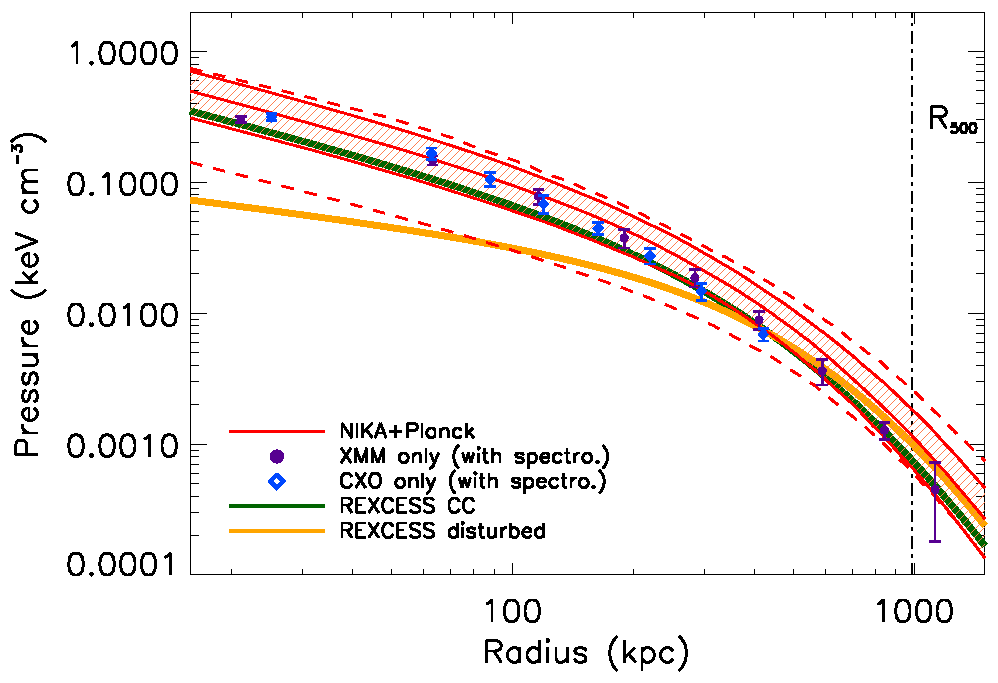
\includegraphics[height=6.3cm]{Figure/ICM_pressure_profile_xray.pdf}
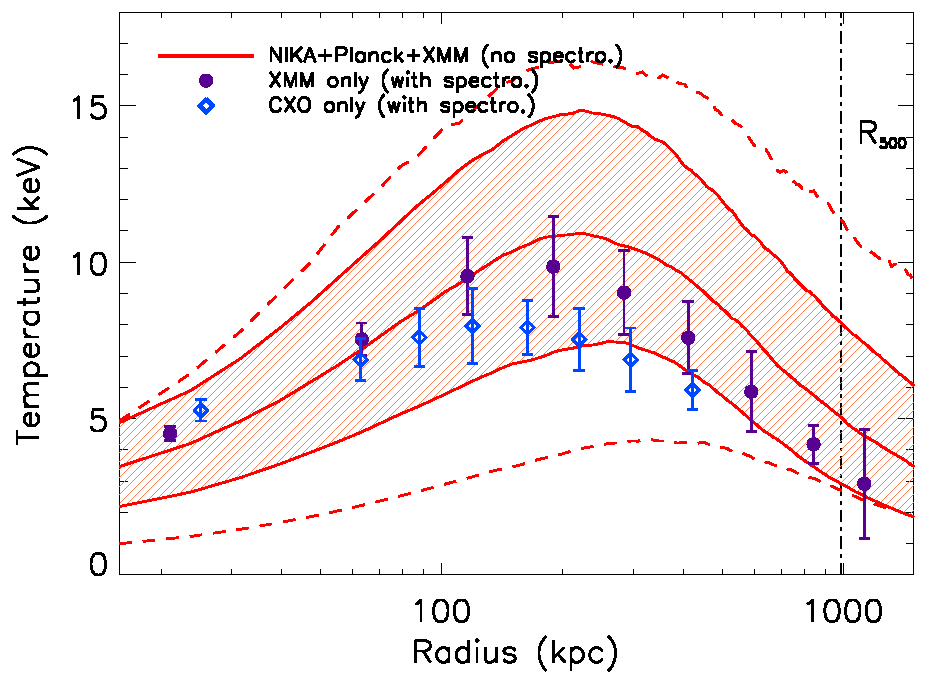
\includegraphics[height=6.3cm]{Figure/ICM_temperature_profile.pdf}
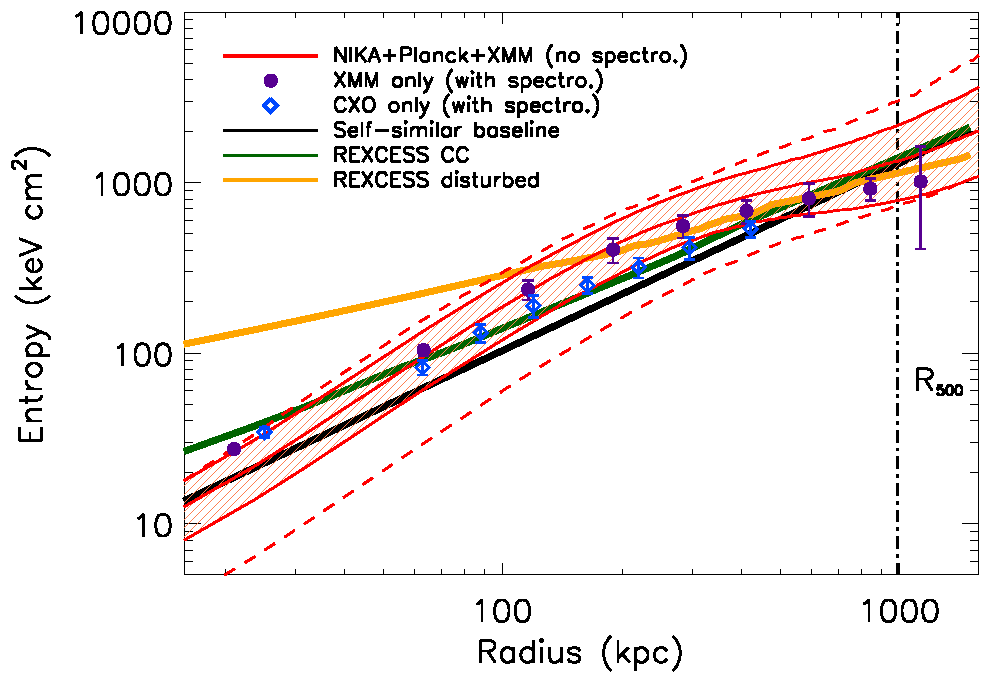
\includegraphics[height=6.3cm]{Figure/ICM_entropy_profile.pdf}
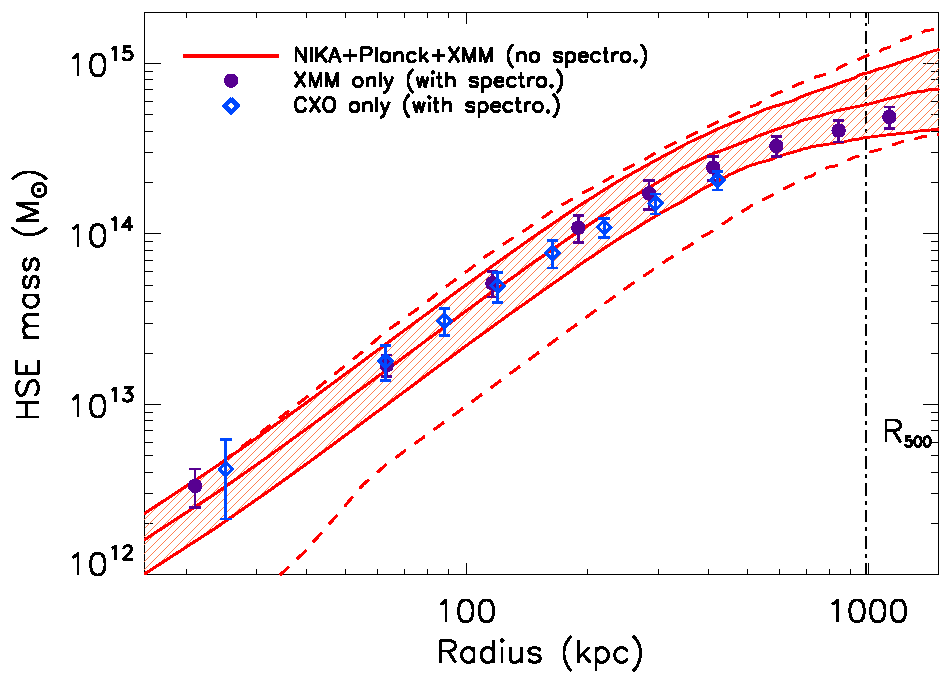
\includegraphics[height=6.3cm]{Figure/ICM_mass_profile.pdf}
\caption{\DIFaddbeginFL \footnotesize \DIFaddendFL MCMC constraints on the deprojected radial profiles of the pressure (top left), the temperature (top right), the entropy (bottom left), and the hydrostatic mass (bottom right). The Chandra only and XMM-Newton only measurements are given by the blue diamonds and the purple dots, respectively. The red shaded area \DIFdelbeginFL \DIFdelFL{provides }\DIFdelendFL \DIFaddbeginFL \DIFaddFL{shows }\DIFaddendFL the MCMC 68\% confidence limit from model M2, the central solid line corresponding to the best-fit model. The two red dashed lines give the upper and lower limits allowed considering all three models M1, M2 and M3 (see Fig.~\ref{fig:MACSJ1424_pressure_point_source}). In the case of the pressure profile, the constraint is driven by the NIKA and Planck tSZ data. Nevertheless, it also depends slightly on the X-ray derived electronic density since we correct for the relativistic corrections using the temperature computed from the pressure and the density, when comparing a given model to the data. We also \DIFdelbeginFL \DIFdelFL{provide }\DIFdelendFL \DIFaddbeginFL \DIFaddFL{show }\DIFaddendFL the pressure \citep{arnaud2010} and entropy \citep{pratt2010} profiles of both cool core (green solid line) and morphologically disturbed (orange solid line) clusters based on \DIFdelbeginFL \DIFdelFL{REXCESS}\DIFdelendFL \DIFaddbeginFL \rexcess\DIFaddendFL , a representative sample of nearby X-ray clusters. \DIFdelbeginFL \DIFdelFL{In }\DIFdelendFL \DIFaddbeginFL \DIFaddFL{For }\DIFaddendFL the \DIFdelbeginFL \DIFdelFL{case of the }\DIFdelendFL entropy profile, the self-similar expectation from non-radiative simulations from \cite{voit2005b} is also represented as a black solid line.}
\label{fig:MACSJ1424_MCMC_tk_profile}
\end{figure*}

%---------- Mass and Ytot
\DIFdelbegin \DIFdel{In addition to the cluster thermodynamics, the assumption of the hydrostatic equilibrium allows us to }\DIFdelend \DIFaddbegin \DIFadd{We can }\DIFaddend derive the mass profile \DIFdelbegin \DIFdel{of the cluster}\DIFdelend \DIFaddbegin \DIFadd{assuming hydrostatic equilibrium}\DIFaddend , as described in Sect.~\ref{sec:modeling}. The bottom right panel of \DIFdelbegin \DIFdel{figure }\DIFdelend \DIFaddbegin \DIFadd{Fig.~}\DIFaddend \ref{fig:MACSJ1424_MCMC_tk_profile} compares the constraints obtained when combining the X-ray and tSZ data with \DIFdelbegin \DIFdel{the }\DIFdelend \DIFaddbegin \DIFadd{those obtained using }\DIFaddend X-ray \DIFdelbegin \DIFdel{only ones. All the }\DIFdelend \DIFaddbegin \DIFadd{data only. The }\DIFaddend constraints are fully compatible \DIFaddbegin \DIFadd{at all scales }\DIFaddend within the 68\% confidence limit\DIFdelbegin \DIFdel{at all scales. By comparing the integrated mass profile to the Universe critical density at the cluster redshift, we obtain }\DIFdelend \DIFaddbegin \DIFadd{. We obtained }\DIFaddend $R_{500} = 1123^{+328}_{-187}$ kpc, which gives $M_{500} = 6.9^{+6.5}_{-2.9}  \times 10^{14} {\rm M}_{\odot}$, in the case of model M3. These results are fully consistent with \DIFdelbegin \DIFdel{the one obtained by }\DIFdelend \DIFaddbegin \DIFadd{those obtained from }\DIFaddend XMM-Newton \DIFdelbegin \DIFdel{only }\DIFdelend \DIFaddbegin \DIFadd{data only: }\DIFaddend ($R_{500} = 986 \pm 10$ kpc and $M_{500} = 4.9 \pm 0.15 \times 10^{14} {\rm M}_{\odot}$), but \DIFdelbegin \DIFdel{present large }\DIFdelend \DIFaddbegin \DIFadd{with larger }\DIFaddend uncertainties. The total integrated Compton parameter \DIFdelbegin \DIFdel{is }\DIFdelend \DIFaddbegin \DIFadd{was }\DIFaddend constrained to be $Y_{\rm tot} = 0.85^{+0.61}_{-0.30} \times 10^{-3}$ arcmin$^2$, in agreement \DIFaddbegin \DIFadd{with, }\DIFaddend but slightly larger than the Planck value \DIFdelbegin \DIFdel{. In table~\ref{tab:summary}, we }\DIFdelend \DIFaddbegin \DIFadd{from aperture photometry. We }\DIFaddend summarize the main recovered properties of \mbox{MACS~J1423.8+2404} \DIFaddbegin \DIFadd{in Table~\ref{tab:summary}}\DIFaddend .
\begin{table}[h]
\caption{Summary of the recovered properties of \mbox{MACS~J1423.8+2404}.}
\begin{center}
\begin{tabular}{cc}
\hline
\hline
$M_{500, {\rm X \ only}}$ & $4.9 \pm 0.15 \times 10^{14} {\rm M}_{\odot}$ \\
$M_{500, {\rm X/tSZ}}$ & $6.9^{+6.5}_{-2.9}  \times 10^{14} {\rm M}_{\odot}$\\
$R_{500, {\rm X \ only}}$ & $986 \pm 10$ kpc\\
$R_{500, {\rm X/tSZ}}$ & $1123^{+328}_{-187}$ kpc\\
$\theta_{500, {\rm X \ only}}$ & $2.50 \pm 0.03$ arcmin \\
$\theta_{500, {\rm X/tSZ}}$ & $2.85^{+0.83}_{-0.47}$ arcmin\\
$Y_{\rm tot}$ & $0.85^{+0.61}_{-0.30} \times 10^{-3}$ arcmin$^2$ \\
\hline
\end{tabular}
\end{center}
\label{tab:summary}
\end{table}

%---------- Discusion
\DIFdelbegin \DIFdel{Both XMM-Newton and Chandra }\DIFdelend \DIFaddbegin \DIFadd{The X-ray }\DIFaddend results present error bars smaller than those derived from NIKA+Planck tSZ data. Nevertheless, we emphasize that both X-ray datasets are particularly exceptional for this cluster (about 30 hours of exposure time for both instruments), while the tSZ ones have been obtained with only 1.47 hours on target. Even in this situation, NIKA already provides essential \DIFdelbegin \DIFdel{informations }\DIFdelend \DIFaddbegin \DIFadd{information }\DIFaddend that allows the reconstruction of the thermodynamical structure of the cluster to reasonable accuracy\DIFdelbegin \DIFdel{when combined to }\DIFdelend \DIFaddbegin \DIFadd{, especially when combined with }\DIFaddend X-ray  \DIFdelbegin \DIFdel{derived }\DIFdelend electronic density.

%###############################################################################################
%##########################                DISCUSSION AND CONCLUSION                ##########################%###############################################################################################
\section{Conclusions and \DIFdelbegin \DIFdel{prospectives}\DIFdelend \DIFaddbegin \DIFadd{perspectives}\DIFaddend }\label{sec:conclusions}
%++++++++++ Prospectives
\subsection{Conclusions}
%---------- NIKA observations
The cluster of galaxies \mbox{MACS~J1423.8+2404} was observed at 150 and 260~GHz using the NIKA camera at the IRAM 30-meter telescope. The target \DIFdelbegin \DIFdel{is }\DIFdelend \DIFaddbegin \DIFadd{was }\DIFaddend detected at 150~GHz in only 1.47 hours and the data show evidence for the presence of a contaminating central point source, as expected from \DIFaddbegin \DIFadd{previous }\DIFaddend radio observations. The 260~GHz NIKA band allows the \DIFaddbegin \DIFadd{further }\DIFaddend identification of two sub-millimeter contaminant galaxies.

%---------- Multi-wavelenght observations
\DIFaddbegin \DIFadd{The }\DIFaddend NIKA observations were combined \DIFdelbegin \DIFdel{to }\DIFdelend \DIFaddbegin \DIFadd{with }\DIFaddend external datasets taken \DIFdelbegin \DIFdel{at }\DIFdelend \DIFaddbegin \DIFadd{in }\DIFaddend multiple wavelengths to investigate the cluster morphology and the dynamical state of the gas. The object \mbox{MACS~J1423.8+2404} is a typical cool core, which appears to be relaxed and elliptical. A total of 17 sub-millimeter sources were identified in the NIKA field using Herschel data, and two radio sources were known from external radio observations.

%--------- Sources
The fluxes of the two radio sources \DIFdelbegin \DIFdel{have been }\DIFdelend \DIFaddbegin \DIFadd{were }\DIFaddend extrapolated to the NIKA bands by fitting a power law SED to external photometric measurements. The sub-millimeter sources were extrapolated to the NIKA bands by modeling their SED with a grey-body spectrum and \DIFdelbegin \DIFdel{fitting jointly the Hershel satellite }\DIFdelend \DIFaddbegin \DIFadd{by jointly fitting the Hershel }\DIFaddend and NIKA photometric data. This work shows the \DIFdelbegin \DIFdel{strong }\DIFdelend \DIFaddbegin \DIFadd{excellent }\DIFaddend complementarity between the two instruments in terms of frequency coverage and angular resolution. \DIFdelbegin \DIFdel{The comparison }\DIFdelend \DIFaddbegin \DIFadd{Comparison }\DIFaddend of the flux density derived \DIFaddbegin \DIFadd{directly }\DIFaddend from NIKA data  \DIFdelbegin \DIFdel{directly shows  a }\DIFdelend \DIFaddbegin \DIFadd{shows  }\DIFaddend good agreement with the expectation from \DIFdelbegin \DIFdel{the point sources extrapolated }\DIFdelend \DIFaddbegin \DIFadd{extrapolated point source }\DIFaddend fluxes at the same frequencies. The contamination from point sources can, therefore, be estimated and subtracted from the tSZ map, if external data are available at complementary wavelengths.

%---------- Profile
The pressure profile of \mbox{MACS~J1423.8+2404} was then measured by modeling and \DIFdelbegin \DIFdel{fitting jointly }\DIFdelend \DIFaddbegin \DIFadd{jointly fitting }\DIFaddend the NIKA and Planck (i.e. $Y_{\rm tot}$) data. We have evaluated the impact of the point \DIFdelbegin \DIFdel{sources }\DIFdelend \DIFaddbegin \DIFadd{source }\DIFaddend contamination on its reconstruction. We find that neglecting the sources leads to an overall underestimate of the profile, which is small compared to the error bars in the case of the available data, but \DIFaddbegin \DIFadd{which }\DIFaddend could become significant when deeper tSZ observations are available. Moreover, in the case of the presence of a point source at the cluster center with no strong priors on its flux, the inner pressure profile remains poorly constrained by the data. Consequently, the \DIFdelbegin \DIFdel{morphology }\DIFdelend \DIFaddbegin \DIFadd{morphological characteristics }\DIFaddend of the cluster could be \DIFdelbegin \DIFdel{also be }\DIFdelend misunderstood in such \DIFdelbegin \DIFdel{case}\DIFdelend \DIFaddbegin \DIFadd{cases}\DIFaddend . We used XMM-Newton and Chandra X-ray observations to derive the cluster thermodynamical radial distributions. The deprojected electronic density has been combined \DIFdelbegin \DIFdel{to }\DIFdelend \DIFaddbegin \DIFadd{with }\DIFaddend the tSZ data, \DIFdelbegin \DIFdel{which provides }\DIFdelend \DIFaddbegin \DIFadd{providing }\DIFaddend a measurement of the pressure, \DIFaddbegin \DIFadd{and used }\DIFaddend to infer the temperature and the entropy profiles. The X-ray only (including spectroscopy) and the tSZ+X-ray (without spectroscopy) constraints are consistent within \DIFdelbegin \DIFdel{error bars}\DIFdelend \DIFaddbegin \DIFadd{their uncertainties}\DIFaddend , and confirm that \mbox{MACS~J1423.8+2404} is a relaxed cool core cluster.

%++++++++++ Prospectives
\subsection{Prospect for NIKA2 observations}
%---------- Prospect for NIKA2
These observations and the present analysis are part of the NIKA tSZ pilot study aiming at characterizing the \DIFdelbegin \DIFdel{outcomes of the }\DIFdelend \DIFaddbegin \DIFadd{potential outcomes of }\DIFaddend future NIKA2 tSZ observations.

Clusters are crowded environments, therefore, in high angular resolution tSZ observations \DIFdelbegin \DIFdel{(}\DIFdelend like those of NIKA2 \DIFdelbegin \DIFdel{) }\DIFdelend we expect the detection of a large number of point sources, as demonstrated in \cite{adam2013}, \cite{adam2014} and in the present work. These sources are a contaminant in the context of tSZ studies. We have shown here that their contribution can be estimated and accounted for if external data are available. Sub-millimeter point sources should not be a problem because they can be identified at 260~GHz and marginalized over at 150~GHz. They can even be masked without removing the information on the \DIFaddbegin \DIFadd{tSZ }\DIFaddend profile. Radio point sources can be more problematic. Unless they are as strong as the tSZ signal, they can only be identified using external data. They are generally correlated with the central BCG and will \DIFdelbegin \DIFdel{refrain }\DIFdelend \DIFaddbegin \DIFadd{prevent  }\DIFaddend NIKA2 \DIFdelbegin \DIFdel{to put }\DIFdelend \DIFaddbegin \DIFadd{from putting }\DIFaddend any constraint on the \DIFdelbegin \DIFdel{cluster core pressure }\DIFdelend \DIFaddbegin \DIFadd{core pressure distribution }\DIFaddend unless their SED is well measured at lower frequencies. If no external data are available, the removal of the contaminants will require the use of extra high angular resolution observations obtained with interferometers at similar frequencies, such as the IRAM NOrthern Extended Millimeter Array (NOEMA)\footnote{\url{http://iram-institute.org/EN/noema-project.php}}. 

Point sources around clusters are also interesting in themselves and the high complementarity between Herschel and NIKA could be used, for example, to search for distant lensed galaxies \citep[see for example][]{egami2010} or to study star formation at high redshift. This should be an extra outcome of the NIKA2 tSZ observations.

The present work has also shown how X-ray and tSZ data can be used to constrain the temperature and the entropy profiles of galaxy clusters independently from X-ray spectroscopy, using the density and pressure profiles. Moving to high redshift, X-ray \DIFdelbegin \DIFdel{spectroscopy, which is necessary to derive the electronic temperature, gets }\DIFdelend \DIFaddbegin \DIFadd{observations become }\DIFaddend time expensive and high-quality X-ray mapping becomes challenging, due to the redshift dimming. In this context, the results obtained in this study show that we are able to constrain the ICM thermodynamics with a good accuracy by combining resolved NIKA tSZ observations and X-ray mapping. This will be particularly important for \DIFdelbegin \DIFdel{NIKA2 distant clusters }\DIFdelend \DIFaddbegin \DIFadd{distant clusters observed with NIKA2}\DIFaddend , for which we will not benefit from deep \DIFdelbegin \DIFdel{enough }\DIFdelend X-ray observations \DIFaddbegin \DIFadd{tuned for spatially resolved X-ray spectroscopy}\DIFaddend , and where only a mean temperature can be obtained from X-ray data. In addition, X-ray constraints on the cluster thermodynamics directly depend on the energy calibration of the instrument, which \DIFdelbegin \DIFdel{is quite often a }\DIFdelend \DIFaddbegin \DIFadd{can be }\DIFaddend source of discrepancy\DIFdelbegin \DIFdel{between XMM-Newton and Chandra observations \mbox{%DIFAUXCMD
\citep[see for example the recent work of][]{schellenberger2015}}%DIFAUXCMD
}\DIFdelend . NIKA tSZ data offer a third independent measurement, independent from X-ray spectroscopy\DIFdelbegin \DIFdel{and related systematics}\DIFdelend , providing a cross check of the temperature measurement of clusters. This can help reducing the systematic effects affecting all these observations, which are essential for mass estimates when using clusters as a cosmological probe.

%###############################################################################################
%##########################                       ACKNOWLEDGEMENTS                        ##########################%###############################################################################################
\begin{acknowledgements}
We thank Marco De Petris for useful comments.
We would like to thank the IRAM staff for their support during the NIKA campaign.
We thank Karin Dassas for helping us obtaining the Herschel data.
This work has been partially funded by the Foundation Nanoscience Grenoble, the ANR under the contracts "MKIDS" and "NIKA". 
This work has been partially supported by the LabEx FOCUS ANR-11-LABX-0013. 
This work has benefited from the support of the European Research Council Advanced Grant ORISTARS under the European Union's Seventh Framework Program (Grant Agreement no. 291294).
\DIFaddbegin \DIFadd{This work has benefitted from the support of the European Research Council Advanced Grant M2C under the European Union’s Seventh Framework Programme (Grant Agreement no. 340519).
}\DIFaddend The NIKA dilution cryostat was designed and built at the Institut N\'eel. In particular, we acknowledge the crucial contribution of the Cryogenics Group and, in particular Gregory Garde, Henri Rodenas, Jean Paul Leggeri, and Philippe Camus. 
We acknowledge the use of the IGLO-HESIOD service from the Integrated Data \& Operation Center (IDOC). Support for IDOC is provided by CNRS \& CNES. 
R. A. would like to thank the ENIGMASS French LabEx for funding this work. 
B. C. acknowledges support from the CNES post-doctoral fellowship program. 
A. R. acknowledges support from the CNES doctoral fellowship program. 
E. P. acknowledges the support of the French Agence Nationale de la Recherche under grant ANR-11-BD56-015.
\end{acknowledgements}

\DIFdelbegin %DIFDELCMD < \begin{thebibliography}{80}
%DIFDELCMD < %%%
\DIFdelend \DIFaddbegin \begin{thebibliography}{79}
\DIFaddend \expandafter\ifx\csname natexlab\endcsname\relax\def\natexlab#1{#1}\fi

\bibitem[{{Adam} {et~al.}(2015){Adam}, {Comis}, {Mac{\'{\i}}as-P{\'e}rez},
  {Adane}, {Ade}, {Andr{\'e}}, {Beelen}, {Belier}, {Beno{\^i}t}, {Bideaud},
  {Billot}, {Blanquer}, {Bourrion}, {Calvo}, {Catalano}, {Coiffard},
  {Cruciani}, {D'Addabbo}, {D{\'e}sert}, {Doyle}, {Goupy}, {Kramer},
  {Leclercq}, {Martino}, {Mauskopf}, {Mayet}, {Monfardini}, {Pajot}, {Pascale},
  {Perotto}, {Pointecouteau}, {Ponthieu}, {Rev{\'e}ret}, {Ritacco},
  {Rodriguez}, {Savini}, {Schuster}, {Sievers}, {Tucker}, \&
  {Zylka}}]{adam2014}
{Adam}, R. {et~al.} 2015, \aap, 576, A12, 1410.2808

\bibitem[{{Adam} {et~al.}(2014){Adam}, {Comis}, {Mac{\'{\i}}as-P{\'e}rez},
  {Adane}, {Ade}, {Andr{\'e}}, {Beelen}, {Belier}, {Beno{\^i}t}, {Bideaud},
  {Billot}, {Boudou}, {Bourrion}, {Calvo}, {Catalano}, {Coiffard}, {D'Addabbo},
  {D{\'e}sert}, {Doyle}, {Goupy}, {Kramer}, {Leclercq}, {Martino}, {Mauskopf},
  {Mayet}, {Monfardini}, {Pajot}, {Pascale}, {Perotto}, {Pointecouteau},
  {Ponthieu}, {Rev{\'e}ret}, {Rodriguez}, {Savini}, {Schuster}, {Sievers},
  {Tucker}, \& {Zylka}}]{adam2013}
------. 2014, \aap, 569, A66, 1310.6237

\bibitem[{{Arnaud} {et~al.}(2001){Arnaud}, {Neumann}, {Aghanim}, {Gastaud},
  {Majerowicz}, \& {Hughes}}]{arnaud2001}
{Arnaud}, M., {Neumann}, D.~M., {Aghanim}, N., {Gastaud}, R., {Majerowicz}, S.,
  \& {Hughes}, J.~P. 2001, \aap, 365, L80, astro-ph/0011198

\bibitem[{{Arnaud} {et~al.}(2010){Arnaud}, {Pratt}, {Piffaretti},
  {B{\"o}hringer}, {Croston}, \& {Pointecouteau}}]{arnaud2010}
{Arnaud}, M., {Pratt}, G.~W., {Piffaretti}, R., {B{\"o}hringer}, H., {Croston},
  J.~H., \& {Pointecouteau}, E. 2010, \aap, 517, A92, 0910.1234

\bibitem[{{Becker} {et~al.}(1995){Becker}, {White}, \& {Helfand}}]{becker1995}
{Becker}, R.~H., {White}, R.~L., \& {Helfand}, D.~J. 1995, \apj, 450, 559

\bibitem[{{Birkinshaw}(1999)}]{birkinshaw1999}
{Birkinshaw}, M. 1999, \physrep, 310, 97, arXiv:astro-ph/9808050

\bibitem[{{Bleem} {et~al.}(2014){Bleem}, {Stalder}, {de Haan}, {Aird}, {Allen},
  {Applegate}, {Ashby}, {Bautz}, {Bayliss}, {Benson}, {Bocquet}, {Brodwin},
  {Carlstrom}, {Chang}, {Chiu}, {Cho}, {Clocchiatti}, {Crawford}, {Crites},
  {Desai}, {Dietrich}, {Dobbs}, {Foley}, {Forman}, {George}, {Gladders},
  {Gonzalez}, {Halverson}, {Hennig}, {Hoekstra}, {Holder}, {Holzapfel},
  {Hrubes}, {Jones}, {Keisler}, {Knox}, {Lee}, {Leitch}, {Liu}, {Lueker},
  {Luong-Van}, {Mantz}, {Marrone}, {McDonald}, {McMahon}, {Meyer}, {Mocanu},
  {Mohr}, {Murray}, {Padin}, {Pryke}, {Reichardt}, {Rest}, {Ruel}, {Ruhl},
  {Saliwanchik}, {Saro}, {Sayre}, {Schaffer}, {Schrabback}, {Shirokoff},
  {Song}, {Spieler}, {Stanford}, {Staniszewski}, {Stark}, {Story}, {Stubbs},
  {Vanderlinde}, {Vieira}, {Vikhlinin}, {Williamson}, {Zahn}, \&
  {Zenteno}}]{bleem2014}
{Bleem}, L.~E. {et~al.} 2014, ArXiv e-prints, 1409.0850

\bibitem[{{B{\"o}hringer} {et~al.}(2007){B{\"o}hringer}, {Schuecker}, {Pratt},
  {Arnaud}, {Ponman}, {Croston}, {Borgani}, {Bower}, {Briel}, {Collins},
  {Donahue}, {Forman}, {Finoguenov}, {Geller}, {Guzzo}, {Henry}, {Kneissl},
  {Mohr}, {Matsushita}, {Mullis}, {Ohashi}, {Pedersen}, {Pierini}, {Quintana},
  {Raychaudhury}, {Reiprich}, {Romer}, {Rosati}, {Sabirli}, {Temple}, {Viana},
  {Vikhlinin}, {Voit}, \& {Zhang}}]{bohringer2007}
{B{\"o}hringer}, H. {et~al.} 2007, \aap, 469, 363, astro-ph/0703553

\bibitem[{{B{\"o}hringer} \& {Werner}(2010)}]{bohringer2010}
{B{\"o}hringer}, H., \& {Werner}, N. 2010, \aapr, 18, 127

\bibitem[{{Bonamente} {et~al.}(2012){Bonamente}, {Hasler}, {Bulbul},
  {Carlstrom}, {Culverhouse}, {Gralla}, {Greer}, {Hawkins}, {Hennessy}, {Joy},
  {Kolodziejczak}, {Lamb}, {Landry}, {Leitch}, {Marrone}, {Miller},
  {Mroczkowski}, {Muchovej}, {Plagge}, {Pryke}, {Sharp}, \&
  {Woody}}]{bonamente2012}
{Bonamente}, M. {et~al.} 2012, New Journal of Physics, 14, 025010, 1112.1599

\bibitem[{{Borgani} \& {Kravtsov}(2011)}]{borgani2011}
{Borgani}, S., \& {Kravtsov}, A. 2011, Advanced Science Letters, 4, 204,
  0906.4370

\bibitem[{{Bourrion} {et~al.}(2011){Bourrion}, {Bideaud}, {Benoit}, {Cruciani},
  {Macias-Perez}, {Monfardini}, {Roesch}, {Swenson}, \&
  {Vescovi}}]{bourion2011}
{Bourrion}, O. {et~al.} 2011, JINST, 6, P06012, 1102.1314

\bibitem[{{Bourrion} {et~al.}(2012){Bourrion}, {Vescovi}, {Bouly}, {Benoit},
  {Calvo}, {Gallin-Martel}, {Macias-Perez}, \& {Monfardini}}]{bourrion2012}
{Bourrion}, O., {Vescovi}, C., {Bouly}, J.~L., {Benoit}, A., {Calvo}, M.,
  {Gallin-Martel}, L., {Macias-Perez}, J.~F., \& {Monfardini}, A. 2012, Journal
  of Instrumentation, 7, 7014, 1204.1415

\bibitem[{{Calvo} {et~al.}(2013){Calvo}, {Roesch}, {D{\'e}sert}, {Monfardini},
  {Benoit}, {Mauskopf}, {Ade}, {Boudou}, {Bourrion}, {Camus}, {Cruciani},
  {Doyle}, {Hoffmann}, {Leclercq}, {Macias-Perez}, {Ponthieu}, {Schuster},
  {Tucker}, \& {Vescovi}}]{calvo2012}
{Calvo}, M. {et~al.} 2013, \aap, 551, L12

\bibitem[{{Cantalupo} {et~al.}(2010){Cantalupo}, {Borrill}, {Jaffe}, {Kisner},
  \& {Stompor}}]{cantalupo2010}
{Cantalupo}, C.~M., {Borrill}, J.~D., {Jaffe}, A.~H., {Kisner}, T.~S., \&
  {Stompor}, R. 2010, \apjs, 187, 212, 0906.1775

\bibitem[{{Carlstrom} {et~al.}(2002){Carlstrom}, {Holder}, \&
  {Reese}}]{carlstrom2002}
{Carlstrom}, J.~E., {Holder}, G.~P., \& {Reese}, E.~D. 2002, \araa, 40, 643,
  arXiv:astro-ph/0208192

\bibitem[{{Catalano} {et~al.}(2014){Catalano}, {Calvo}, {Ponthieu}, {Adam},
  {Adane}, {Ade}, {Andr{\'e}}, {Beelen}, {Belier}, {Beno{\^i}t}, {Bideaud},
  {Billot}, {Boudou}, {Bourrion}, {Coiffard}, {Comis}, {D'Addabbo},
  {D{\'e}sert}, {Doyle}, {Goupy}, {Kramer}, {Leclercq},
  {Mac{\'{\i}}as-P{\'e}rez}, {Martino}, {Mauskopf}, {Mayet}, {Monfardini},
  {Pajot}, {Pascale}, {Perotto}, {Rev{\'e}ret}, {Rodriguez}, {Savini},
  {Schuster}, {Sievers}, {Tucker}, \& {Zylka}}]{catalano2014}
{Catalano}, A. {et~al.} 2014, \aap, 569, A9, 1402.0260

\bibitem[{{Cavagnolo} {et~al.}(2009){Cavagnolo}, {Donahue}, {Voit}, \&
  {Sun}}]{cavagnolo2009}
{Cavagnolo}, K.~W., {Donahue}, M., {Voit}, G.~M., \& {Sun}, M. 2009, \apjs,
  182, 12, 0902.1802

\bibitem[{{Coble} {et~al.}(2007){Coble}, {Bonamente}, {Carlstrom}, {Dawson},
  {Hasler}, {Holzapfel}, {Joy}, {La Roque}, {Marrone}, \& {Reese}}]{coble2007}
{Coble}, K. {et~al.} 2007, \aj, 134, 897, astro-ph/0608274

\bibitem[{{Condon} {et~al.}(1998){Condon}, {Cotton}, {Greisen}, {Yin},
  {Perley}, {Taylor}, \& {Broderick}}]{condon1998}
{Condon}, J.~J., {Cotton}, W.~D., {Greisen}, E.~W., {Yin}, Q.~F., {Perley},
  R.~A., {Taylor}, G.~B., \& {Broderick}, J.~J. 1998, \aj, 115, 1693

\bibitem[{{Croston} {et~al.}(2006){Croston}, {Arnaud}, {Pointecouteau}, \&
  {Pratt}}]{croston2006}
{Croston}, J.~H., {Arnaud}, M., {Pointecouteau}, E., \& {Pratt}, G.~W. 2006,
  \aap, 459, 1007, astro-ph/0608700

\bibitem[{{da Silva} {et~al.}(2004){da Silva}, {Kay}, {Liddle}, \&
  {Thomas}}]{dasilva2004}
{da Silva}, A.~C., {Kay}, S.~T., {Liddle}, A.~R., \& {Thomas}, P.~A. 2004,
  \mnras, 348, 1401, astro-ph/0308074

\DIFdelbegin %DIFDELCMD < \bibitem[{{Del Popolo}(2012)}]{delpopolo2012}
%DIFDELCMD < {%%%
\DIFdel{Del Popolo}%DIFDELCMD < }%%%
\DIFdel{, A. 2012, }%DIFDELCMD < \mnras%%%
\DIFdel{, 424, 38, 1204.4439
}%DIFDELCMD < 

%DIFDELCMD < %%%
\DIFdelend \bibitem[{{Ebeling} {et~al.}(2001){Ebeling}, {Edge}, \& {Henry}}]{ebeling2001}
{Ebeling}, H., {Edge}, A.~C., \& {Henry}, J.~P. 2001, \apj, 553, 668,
  astro-ph/0009101

\bibitem[{{Egami} {et~al.}(2010){Egami}, {Rex}, {Rawle},
  {P{\'e}rez-Gonz{\'a}lez}, {Richard}, {Kneib}, {Schaerer}, {Altieri},
  {Valtchanov}, {Blain}, {Fadda}, {Zemcov}, {Bock}, {Boone}, {Bridge},
  {Clement}, {Combes}, {Dessauges-Zavadsky}, {Dowell}, {Ilbert}, {Ivison},
  {Jauzac}, {Lutz}, {Metcalfe}, {Omont}, {Pell{\'o}}, {Pereira}, {Rieke},
  {Rodighiero}, {Smail}, {Smith}, {Tramoy}, {Walth}, {van der Werf}, \&
  {Werner}}]{egami2010}
{Egami}, E. {et~al.} 2010, \aap, 518, L12, 1005.3820

\bibitem[{{Ghizzardi}(2001)}]{ghizzardi2001}
{Ghizzardi}, S. 2001, XMM-SOC-CAL-TN-0022

\bibitem[{{Giacconi} {et~al.}(2001){Giacconi}, {Rosati}, {Tozzi}, {Nonino},
  {Hasinger}, {Norman}, {Bergeron}, {Borgani}, {Gilli}, {Gilmozzi}, \&
  {Zheng}}]{giacconi2001}
{Giacconi}, R. {et~al.} 2001, \apj, 551, 624, astro-ph/0007240

\bibitem[{{Griffin} {et~al.}(2010){Griffin}, {Abergel}, {Abreu}, {Ade},
  {Andr{\'e}}, {Augueres}, {Babbedge}, {Bae}, {Baillie}, {Baluteau}, {Barlow},
  {Bendo}, {Benielli}, {Bock}, {Bonhomme}, {Brisbin}, {Brockley-Blatt},
  {Caldwell}, {Cara}, {Castro-Rodriguez}, {Cerulli}, {Chanial}, {Chen},
  {Clark}, {Clements}, {Clerc}, {Coker}, {Communal}, {Conversi}, {Cox},
  {Crumb}, {Cunningham}, {Daly}, {Davis}, {de Antoni}, {Delderfield}, {Devin},
  {di Giorgio}, {Didschuns}, {Dohlen}, {Donati}, {Dowell}, {Dowell}, {Duband},
  {Dumaye}, {Emery}, {Ferlet}, {Ferrand}, {Fontignie}, {Fox}, {Franceschini},
  {Frerking}, {Fulton}, {Garcia}, {Gastaud}, {Gear}, {Glenn}, {Goizel},
  {Griffin}, {Grundy}, {Guest}, {Guillemet}, {Hargrave}, {Harwit}, {Hastings},
  {Hatziminaoglou}, {Herman}, {Hinde}, {Hristov}, {Huang}, {Imhof}, {Isaak},
  {Israelsson}, {Ivison}, {Jennings}, {Kiernan}, {King}, {Lange}, {Latter},
  {Laurent}, {Laurent}, {Leeks}, {Lellouch}, {Levenson}, {Li}, {Li},
  {Lilienthal}, {Lim}, {Liu}, {Lu}, {Madden}, {Mainetti}, {Marliani}, {McKay},
  {Mercier}, {Molinari}, {Morris}, {Moseley}, {Mulder}, {Mur}, {Naylor},
  {Nguyen}, {O'Halloran}, {Oliver}, {Olofsson}, {Olofsson}, {Orfei}, {Page},
  {Pain}, {Panuzzo}, {Papageorgiou}, {Parks}, {Parr-Burman}, {Pearce},
  {Pearson}, {P{\'e}rez-Fournon}, {Pinsard}, {Pisano}, {Podosek}, {Pohlen},
  {Polehampton}, {Pouliquen}, {Rigopoulou}, {Rizzo}, {Roseboom}, {Roussel},
  {Rowan-Robinson}, {Rownd}, {Saraceno}, {Sauvage}, {Savage}, {Savini},
  {Sawyer}, {Scharmberg}, {Schmitt}, {Schneider}, {Schulz}, {Schwartz},
  {Shafer}, {Shupe}, {Sibthorpe}, {Sidher}, {Smith}, {Smith}, {Smith},
  {Spencer}, {Stobie}, {Sudiwala}, {Sukhatme}, {Surace}, {Stevens}, {Swinyard},
  {Trichas}, {Tourette}, {Triou}, {Tseng}, {Tucker}, {Turner}, {Vaccari},
  {Valtchanov}, {Vigroux}, {Virique}, {Voellmer}, {Walker}, {Ward}, {Waskett},
  {Weilert}, {Wesson}, {White}, {Whitehouse}, {Wilson}, {Winter}, {Woodcraft},
  {Wright}, {Xu}, {Zavagno}, {Zemcov}, {Zhang}, \& {Zonca}}]{griffin2010}
{Griffin}, M.~J. {et~al.} 2010, \aap, 518, L3, 1005.5123

\bibitem[{{Guennou} {et~al.}(2014){Guennou}, {Adami}, {Durret}, {Lima Neto},
  {Ulmer}, {Clowe}, {LeBrun}, {Martinet}, {Allam}, {Annis}, {Basa}, {Benoist},
  {Biviano}, {Cappi}, {Cypriano}, {Gavazzi}, {Halliday}, {Ilbert}, {Jullo},
  {Just}, {Limousin}, {M{\'a}rquez}, {Mazure}, {Murphy}, {Plana}, {Rostagni},
  {Russeil}, {Schirmer}, {Slezak}, {Tucker}, {Zaritsky}, \&
  {Ziegler}}]{guennou2014}
{Guennou}, L. {et~al.} 2014, \aap, 561, A112, 1311.6922

\bibitem[{{Hasselfield} {et~al.}(2013){Hasselfield}, {Hilton}, {Marriage},
  {Addison}, {Barrientos}, {Battaglia}, {Battistelli}, {Bond}, {Crichton},
  {Das}, {Devlin}, {Dicker}, {Dunkley}, {D{\"u}nner}, {Fowler}, {Gralla},
  {Hajian}, {Halpern}, {Hincks}, {Hlozek}, {Hughes}, {Infante}, {Irwin},
  {Kosowsky}, {Marsden}, {Menanteau}, {Moodley}, {Niemack}, {Nolta}, {Page},
  {Partridge}, {Reese}, {Schmitt}, {Sehgal}, {Sherwin}, {Sievers}, {Sif{\'o}n},
  {Spergel}, {Staggs}, {Swetz}, {Switzer}, {Thornton}, {Trac}, \&
  {Wollack}}]{hasselfield2013}
{Hasselfield}, M. {et~al.} 2013, \jcap, 7, 8, 1301.0816

\bibitem[{{Hlavacek-Larrondo} {et~al.}(2012){Hlavacek-Larrondo}, {Fabian},
  {Edge}, {Ebeling}, {Sanders}, {Hogan}, \& {Taylor}}]{hlavacek_larrondo2012}
{Hlavacek-Larrondo}, J., {Fabian}, A.~C., {Edge}, A.~C., {Ebeling}, H.,
  {Sanders}, J.~S., {Hogan}, M.~T., \& {Taylor}, G.~B. 2012, \mnras, 421, 1360,
  1110.0489

\bibitem[{{Itoh} {et~al.}(1998){Itoh}, {Kohyama}, \& {Nozawa}}]{itoh1998}
{Itoh}, N., {Kohyama}, Y., \& {Nozawa}, S. 1998, \apj, 502, 7,
  arXiv:astro-ph/9712289

\bibitem[{{Kalberla} {et~al.}(2005){Kalberla}, {Burton}, {Hartmann}, {Arnal},
  {Bajaja}, {Morras}, \& {P{\"o}ppel}}]{kalberla2005}
{Kalberla}, P.~M.~W., {Burton}, W.~B., {Hartmann}, D., {Arnal}, E.~M.,
  {Bajaja}, E., {Morras}, R., \& {P{\"o}ppel}, W.~G.~L. 2005, \aap, 440, 775,
  astro-ph/0504140

\bibitem[{{Kartaltepe} {et~al.}(2008){Kartaltepe}, {Ebeling}, {Ma}, \&
  {Donovan}}]{kartaltepe2008}
{Kartaltepe}, J.~S., {Ebeling}, H., {Ma}, C.~J., \& {Donovan}, D. 2008, \mnras,
  389, 1240, 0806.4019

\bibitem[{{Kitayama}(2014)}]{kitayama2014}
{Kitayama}, T. 2014, Progress of Theoretical and Experimental Physics, 2014,
  060000, 1404.0870

\bibitem[{{Komatsu} {et~al.}(2001){Komatsu}, {Matsuo}, {Kitayama}, {Hattori},
  {Kawabe}, {Kohno}, {Kuno}, {Schindler}, {Suto}, \& {Yoshikawa}}]{komatsu2001}
{Komatsu}, E. {et~al.} 2001, \pasj, 53, 57, astro-ph/0006293

\bibitem[{{Korngut} {et~al.}(2011){Korngut}, {Dicker}, {Reese}, {Mason},
  {Devlin}, {Mroczkowski}, {Sarazin}, {Sun}, \& {Sievers}}]{korngut2011}
{Korngut}, P.~M. {et~al.} 2011, \apj, 734, 10, 1010.5494

\bibitem[{{LaRoque} {et~al.}(2003){LaRoque}, {Joy}, {Carlstrom}, {Ebeling},
  {Bonamente}, {Dawson}, {Edge}, {Holzapfel}, {Miller}, {Nagai}, {Patel}, \&
  {Reese}}]{laroque2003}
{LaRoque}, S.~J. {et~al.} 2003, \apj, 583, 559

\bibitem[{{Limousin} {et~al.}(2010){Limousin}, {Ebeling}, {Ma}, {Swinbank},
  {Smith}, {Richard}, {Edge}, {Jauzac}, {Kneib}, {Marshall}, \&
  {Schrabback}}]{limousin2010}
{Limousin}, M. {et~al.} 2010, \mnras, 405, 777, 0911.4125

\bibitem[{{Mahdavi} {et~al.}(2013){Mahdavi}, {Hoekstra}, {Babul}, {Bildfell},
  {Jeltema}, \& {Henry}}]{mahdavi2013}
{Mahdavi}, A., {Hoekstra}, H., {Babul}, A., {Bildfell}, C., {Jeltema}, T., \&
  {Henry}, J.~P. 2013, \apj, 767, 116, 1210.3689

\bibitem[{{Martino} {et~al.}(2014){Martino}, {Mazzotta}, {Bourdin}, {Smith},
  {Bartalucci}, {Marrone}, {Finoguenov}, \& {Okabe}}]{martino2014}
{Martino}, R., {Mazzotta}, P., {Bourdin}, H., {Smith}, G.~P., {Bartalucci}, I.,
  {Marrone}, D.~P., {Finoguenov}, A., \& {Okabe}, N. 2014, \mnras, 443, 2342,
  1406.6831

\bibitem[{{Mazzotta} {et~al.}(2004){Mazzotta}, {Rasia}, {Moscardini}, \&
  {Tormen}}]{mazzotta2004}
{Mazzotta}, P., {Rasia}, E., {Moscardini}, L., \& {Tormen}, G. 2004, \mnras,
  354, 10, astro-ph/0404425

\bibitem[{{Monfardini} {et~al.}(2014){Monfardini}, {Adam}, {Adane}, {Ade},
  {Andr{\'e}}, {Beelen}, {Belier}, {Benoit}, {Bideaud}, {Billot}, {Bourrion},
  {Calvo}, {Catalano}, {Coiffard}, {Comis}, {D'Addabbo}, {D{\'e}sert}, {Doyle},
  {Goupy}, {Kramer}, {Leclercq}, {Macias-Perez}, {Martino}, {Mauskopf},
  {Mayet}, {Pajot}, {Pascale}, {Ponthieu}, {Rev{\'e}ret}, {Rodriguez},
  {Savini}, {Schuster}, {Sievers}, {Tucker}, \& {Zylka}}]{monfardini2014}
{Monfardini}, A. {et~al.} 2014, Journal of Low Temperature Physics, 176, 787,
  1310.1230

\bibitem[{{Monfardini} {et~al.}(2011){Monfardini}, {Benoit}, {Bideaud},
  {Swenson}, {Cruciani}, {Camus}, {Hoffmann}, {D{\'e}sert}, {Doyle}, {Ade},
  {Mauskopf}, {Tucker}, {Roesch}, {Leclercq}, {Schuster}, {Endo}, {Baryshev},
  {Baselmans}, {Ferrari}, {Yates}, {Bourrion}, {Macias-Perez}, {Vescovi},
  {Calvo}, \& {Giordano}}]{monfardini2011}
------. 2011, \apjs, 194, 24, 1102.0870

\bibitem[{{Monfardini} {et~al.}(2010){Monfardini}, {Swenson}, {Bideaud},
  {D{\'e}sert}, {Yates}, {Benoit}, {Baryshev}, {Baselmans}, {Doyle}, {Klein},
  {Roesch}, {Tucker}, {Ade}, {Calvo}, {Camus}, {Giordano}, {Guesten},
  {Hoffmann}, {Leclercq}, {Mauskopf}, \& {Schuster}}]{monfardini2010}
------. 2010, \aap, 521, A29, 1004.2209

\bibitem[{{Morandi} {et~al.}(2010){Morandi}, {Pedersen}, \&
  {Limousin}}]{morandi2010}
{Morandi}, A., {Pedersen}, K., \& {Limousin}, M. 2010, \apj, 713, 491,
  0912.2648

\bibitem[{{Motl} {et~al.}(2005){Motl}, {Hallman}, {Burns}, \&
  {Norman}}]{motl2005}
{Motl}, P.~M., {Hallman}, E.~J., {Burns}, J.~O., \& {Norman}, M.~L. 2005,
  \apjl, 623, L63, astro-ph/0502226

\bibitem[{{Mroczkowski} {et~al.}(2015){Mroczkowski}, {Kov{\'a}cs}, {Bulbul},
  {Staguhn}, {Benford}, {Clarke}, {van Weeren}, {Intema}, \&
  {Randall}}]{mroczkowski2015}
{Mroczkowski}, T. {et~al.} 2015, ArXiv e-prints, 1501.05051

\bibitem[{{Nagai}(2006)}]{nagai2006}
{Nagai}, D. 2006, \apj, 650, 538, astro-ph/0512208

\bibitem[{{Nagai} {et~al.}(2007){Nagai}, {Vikhlinin}, \&
  {Kravtsov}}]{nagai2007}
{Nagai}, D., {Vikhlinin}, A., \& {Kravtsov}, A.~V. 2007, \apj, 655, 98,
  arXiv:astro-ph/0609247

\bibitem[{{Planck Collaboration}(2015)}]{planck2014param}
{Planck Collaboration}. 2015, ArXiv e-prints, 1502.01589

\bibitem[{{Planck Collaboration} {et~al.}(2013{\natexlab{a}}){Planck
  Collaboration}, {Ade}, {Aghanim}, {Armitage-Caplan}, {Arnaud}, {Ashdown},
  {Atrio-Barandela}, {Aumont}, {Aussel}, {Baccigalupi}, \&
  et~al.}]{planck2013catalogue}
{Planck Collaboration} {et~al.} 2013{\natexlab{a}}, ArXiv e-prints, 1303.5089

\bibitem[{{Planck Collaboration} {et~al.}(2013{\natexlab{b}}){Planck
  Collaboration}, {Ade}, {Aghanim}, {Armitage-Caplan}, {Arnaud}, {Ashdown},
  {Atrio-Barandela}, {Aumont}, {Baccigalupi}, {Banday}, \&
  et~al.}]{planck2013cluster_count}
------. 2013{\natexlab{b}}, ArXiv e-prints, 1303.5080

\bibitem[{{Planck Collaboration} {et~al.}(2013{\natexlab{c}}){Planck
  Collaboration}, {Ade}, {Aghanim}, {Arnaud}, {Ashdown}, {Atrio-Barandela},
  {Aumont}, {Baccigalupi}, {Balbi}, {Banday}, \&
  et~al.}]{planck2013pressure_profile}
------. 2013{\natexlab{c}}, \aap, 550, A131, 1207.4061

\bibitem[{{Planck Collaboration} {et~al.}(2015{\natexlab{a}}){Planck
  Collaboration}, {Ade}, {Aghanim}, {Arnaud}, {Ashdown}, {Aumont},
  {Baccigalupi}, {Banday}, {Barreiro}, {Barrena}, \& et~al.}]{planck2015XXVII}
------. 2015{\natexlab{a}}, ArXiv e-prints, 1502.01598

\bibitem[{{Planck Collaboration} {et~al.}(2015{\natexlab{b}}){Planck
  Collaboration}, {Aghanim}, {Arnaud}, {Ashdown}, {Aumont}, {Baccigalupi},
  {Banday}, {Barreiro}, {Bartlett}, {Bartolo}, \& et~al.}]{planck2015XXII}
------. 2015{\natexlab{b}}, ArXiv e-prints, 1502.01596

\bibitem[{{Poglitsch} {et~al.}(2010){Poglitsch}, {Waelkens}, {Geis},
  {Feuchtgruber}, {Vandenbussche}, {Rodriguez}, {Krause}, {Renotte}, {van
  Hoof}, {Saraceno}, {Cepa}, {Kerschbaum}, {Agn{\`e}se}, {Ali}, {Altieri},
  {Andreani}, {Augueres}, {Balog}, {Barl}, {Bauer}, {Belbachir}, {Benedettini},
  {Billot}, {Boulade}, {Bischof}, {Blommaert}, {Callut}, {Cara}, {Cerulli},
  {Cesarsky}, {Contursi}, {Creten}, {De Meester}, {Doublier}, {Doumayrou},
  {Duband}, {Exter}, {Genzel}, {Gillis}, {Gr{\"o}zinger}, {Henning},
  {Herreros}, {Huygen}, {Inguscio}, {Jakob}, {Jamar}, {Jean}, {de Jong},
  {Katterloher}, {Kiss}, {Klaas}, {Lemke}, {Lutz}, {Madden}, {Marquet},
  {Martignac}, {Mazy}, {Merken}, {Montfort}, {Morbidelli}, {M{\"u}ller},
  {Nielbock}, {Okumura}, {Orfei}, {Ottensamer}, {Pezzuto}, {Popesso},
  {Putzeys}, {Regibo}, {Reveret}, {Royer}, {Sauvage}, {Schreiber}, {Stegmaier},
  {Schmitt}, {Schubert}, {Sturm}, {Thiel}, {Tofani}, {Vavrek}, {Wetzstein},
  {Wieprecht}, \& {Wiezorrek}}]{poglitsch2010}
{Poglitsch}, A. {et~al.} 2010, \aap, 518, L2, 1005.1487

\bibitem[{{Pointecouteau} {et~al.}(1999){Pointecouteau}, {Giard}, {Benoit},
  {D{\'e}sert}, {Aghanim}, {Coron}, {Lamarre}, \&
  {Delabrouille}}]{pointecouteau1999}
{Pointecouteau}, E., {Giard}, M., {Benoit}, A., {D{\'e}sert}, F.~X., {Aghanim},
  N., {Coron}, N., {Lamarre}, J.~M., \& {Delabrouille}, J. 1999, \apjl, 519,
  L115

\bibitem[{{Ponthieu} {et~al.}(2011){Ponthieu}, {Grain}, \&
  {Lagache}}]{ponthieu2011}
{Ponthieu}, N., {Grain}, J., \& {Lagache}, G. 2011, \aap, 535, A90, 1111.0766

\bibitem[{{Postman} {et~al.}(2012){Postman}, {Coe}, {Ben{\'{\i}}tez},
  {Bradley}, {Broadhurst}, {Donahue}, {Ford}, {Graur}, {Graves}, {Jouvel},
  {Koekemoer}, {Lemze}, {Medezinski}, {Molino}, {Moustakas}, {Ogaz}, {Riess},
  {Rodney}, {Rosati}, {Umetsu}, {Zheng}, {Zitrin}, {Bartelmann}, {Bouwens},
  {Czakon}, {Golwala}, {Host}, {Infante}, {Jha}, {Jimenez-Teja}, {Kelson},
  {Lahav}, {Lazkoz}, {Maoz}, {McCully}, {Melchior}, {Meneghetti}, {Merten},
  {Moustakas}, {Nonino}, {Patel}, {Reg{\"o}s}, {Sayers}, {Seitz}, \& {Van der
  Wel}}]{postman2012}
{Postman}, M. {et~al.} 2012, \apjs, 199, 25, 1106.3328

\bibitem[{{Pratt} {et~al.}(2010){Pratt}, {Arnaud}, {Piffaretti},
  {B{\"o}hringer}, {Ponman}, {Croston}, {Voit}, {Borgani}, \&
  {Bower}}]{pratt2010}
{Pratt}, G.~W. {et~al.} 2010, \aap, 511, A85, 0909.3776

\bibitem[{{Pratt} {et~al.}(2007){Pratt}, {B{\"o}hringer}, {Croston}, {Arnaud},
  {Borgani}, {Finoguenov}, \& {Temple}}]{pratt2007}
{Pratt}, G.~W., {B{\"o}hringer}, H., {Croston}, J.~H., {Arnaud}, M., {Borgani},
  S., {Finoguenov}, A., \& {Temple}, R.~F. 2007, \aap, 461, 71,
  astro-ph/0609480

\bibitem[{{Pratt} {et~al.}(2009){Pratt}, {Croston}, {Arnaud}, \&
  {B{\"o}hringer}}]{pratt2009}
{Pratt}, G.~W., {Croston}, J.~H., {Arnaud}, M., \& {B{\"o}hringer}, H. 2009,
  \aap, 498, 361, 0809.3784

\bibitem[{{Rawle} {et~al.}(2012){Rawle}, {Edge}, {Egami}, {Rex}, {Smith},
  {Altieri}, {Fiedler}, {Haines}, {Pereira}, {P{\'e}rez-Gonz{\'a}lez},
  {Portouw}, {Valtchanov}, {Walth}, {van der Werf}, \& {Zemcov}}]{rawle2012}
{Rawle}, T.~D. {et~al.} 2012, \apj, 747, 29, 1201.1294

\bibitem[{{Reichardt} {et~al.}(2013){Reichardt}, {Stalder}, {Bleem}, {Montroy},
  {Aird}, {Andersson}, {Armstrong}, {Ashby}, {Bautz}, {Bayliss}, {Bazin},
  {Benson}, {Brodwin}, {Carlstrom}, {Chang}, {Cho}, {Clocchiatti}, {Crawford},
  {Crites}, {de Haan}, {Desai}, {Dobbs}, {Dudley}, {Foley}, {Forman}, {George},
  {Gladders}, {Gonzalez}, {Halverson}, {Harrington}, {High}, {Holder},
  {Holzapfel}, {Hoover}, {Hrubes}, {Jones}, {Joy}, {Keisler}, {Knox}, {Lee},
  {Leitch}, {Liu}, {Lueker}, {Luong-Van}, {Mantz}, {Marrone}, {McDonald},
  {McMahon}, {Mehl}, {Meyer}, {Mocanu}, {Mohr}, {Murray}, {Natoli}, {Padin},
  {Plagge}, {Pryke}, {Rest}, {Ruel}, {Ruhl}, {Saliwanchik}, {Saro}, {Sayre},
  {Schaffer}, {Shaw}, {Shirokoff}, {Song}, {Spieler}, {Staniszewski}, {Stark},
  {Story}, {Stubbs}, {{\v S}uhada}, {van Engelen}, {Vanderlinde}, {Vieira},
  {Vikhlinin}, {Williamson}, {Zahn}, \& {Zenteno}}]{reichardt2013}
{Reichardt}, C.~L. {et~al.} 2013, \apj, 763, 127, 1203.5775

\bibitem[{{Savage} \& {Oliver}(2007)}]{savage2007}
{Savage}, R.~S., \& {Oliver}, S. 2007, \apj, 661, 1339, astro-ph/0512597

\bibitem[{{Sayers} {et~al.}(2013{\natexlab{a}}){Sayers}, {Czakon}, {Mantz},
  {Golwala}, {Ameglio}, {Downes}, {Koch}, {Lin}, {Maughan}, {Molnar},
  {Moustakas}, {Mroczkowski}, {Pierpaoli}, {Shitanishi}, {Siegel}, {Umetsu}, \&
  {Van der Pyl}}]{sayers2013b}
{Sayers}, J. {et~al.} 2013{\natexlab{a}}, \apj, 768, 177, 1211.1632

\bibitem[{{Sayers} {et~al.}(2013{\natexlab{b}}){Sayers}, {Mroczkowski},
  {Czakon}, {Golwala}, {Mantz}, {Ameglio}, {Downes}, {Koch}, {Lin}, {Molnar},
  {Moustakas}, {Muchovej}, {Pierpaoli}, {Shitanishi}, {Siegel}, \&
  {Umetsu}}]{sayers2013a}
------. 2013{\natexlab{b}}, \apj, 764, 152, 1209.5129

\DIFdelbegin %DIFDELCMD < \bibitem[{{Schellenberger} {et~al.}(2015){Schellenberger}, {Reiprich},
%DIFDELCMD <   {Lovisari}, {Nevalainen}, \& {David}}]{schellenberger2015}
%DIFDELCMD < %%%
\DIFdelend \DIFaddbegin \bibitem[{{Schellenberger} {et~al.}(2015){Schellenberger}, {Reiprich},
  {Lovisari}, {Nevalainen}, \& {David}}]{sch15}
\DIFaddend {Schellenberger}, G., {Reiprich}, T.~H., {Lovisari}, L., {Nevalainen}, J., \&
  {David}, L. 2015, \aap, 575, A30, 1404.7130

\bibitem[{{Schmidt} \& {Allen}(2007)}]{schmidt2007}
{Schmidt}, R.~W., \& {Allen}, S.~W. 2007, \mnras, 379, 209, astro-ph/0610038

\bibitem[{{Snowden} {et~al.}(1995){Snowden}, {Freyberg}, {Plucinsky},
  {Schmitt}, {Truemper}, {Voges}, {Edgar}, {McCammon}, \&
  {Sanders}}]{snowden1995}
{Snowden}, S.~L. {et~al.} 1995, \apj, 454, 643

\bibitem[{{Sunyaev} \& {Zel'dovich}(1972)}]{sunyaev1972}
{Sunyaev}, R.~A., \& {Zel'dovich}, Y.~B. 1972, \apspr, 4, 173

\bibitem[{{Sunyaev} \& {Zel'dovich}(1980)}]{sunyaev1980}
------. 1980, \araa, 18, 537

\bibitem[{{Vikhlinin}(2006)}]{vikh_multit}
{Vikhlinin}, A. 2006, \apj, 640, 710, astro-ph/0504098

\bibitem[{{Vikhlinin} {et~al.}(2006){Vikhlinin}, {Kravtsov}, {Forman}, {Jones},
  {Markevitch}, {Murray}, \& {Van Speybroeck}}]{vikhlinin2006}
{Vikhlinin}, A., {Kravtsov}, A., {Forman}, W., {Jones}, C., {Markevitch}, M.,
  {Murray}, S.~S., \& {Van Speybroeck}, L. 2006, \apj, 640, 691,
  astro-ph/0507092

\bibitem[{{Voit}(2005)}]{voit2005}
{Voit}, G.~M. 2005, Reviews of Modern Physics, 77, 207, astro-ph/0410173

\bibitem[{{Voit} {et~al.}(2005){Voit}, {Kay}, \& {Bryan}}]{voit2005b}
{Voit}, G.~M., {Kay}, S.~T., \& {Bryan}, G.~L. 2005, \mnras, 364, 909,
  astro-ph/0511252

\bibitem[{{Witzel} {et~al.}(1979){Witzel}, {Pauliny-Toth}, {Nauber}, \&
  {Schmidt}}]{witzel1979}
{Witzel}, A., {Pauliny-Toth}, I.~I.~K., {Nauber}, U., \& {Schmidt}, J. 1979,
  \aj, 84, 942

\bibitem[{{Young} {et~al.}(2014){Young}, {Mroczkowski}, {Romero}, {Sayers},
  {Balestra}, {Clarke}, {Czakon}, {Devlin}, {Dicker}, {Ferrari}, {Girardi},
  {Golwala}, {Intema}, {Korngut}, {Mason}, {Mercurio}, {Nonino}, {Reese},
  {Rosati}, {Sarazin}, \& {Umetsu}}]{young2014}
{Young}, A.~H. {et~al.} 2014, ArXiv e-prints, 1411.0317

\bibitem[{{Zitrin} {et~al.}(2011){Zitrin}, {Broadhurst}, {Barkana}, {Rephaeli},
  \& {Ben{\'{\i}}tez}}]{zitrin2011}
{Zitrin}, A., {Broadhurst}, T., {Barkana}, R., {Rephaeli}, Y., \&
  {Ben{\'{\i}}tez}, N. 2011, \mnras, 410, 1939, 1002.0521

\end{thebibliography}

\end{document}